\documentclass{IEEEtran}

\usepackage[margin=0.5in]{geometry}
\usepackage{graphicx}
\usepackage{titling}
\usepackage{graphicx} % Required for inserting images.
% \usepackage{wrapfig}
\usepackage{subfig}
\usepackage{amsmath}
\usepackage{amssymb}

\begin{document}
\title{
  
\includegraphics[width=1in]{figures/logo.png}\\
  BIO-482 Neuroscience: Cellular Circuit Mechanisms.\\
Cortical Neuron Classification: Leveraging Interpretable Machine Learning Techniques.
}
\author{
  Wesley Monteith-Finas, SCIPER: 324745\\
In collaboration with Marianne Scoglio \& Sander Miesen
}
\maketitle


\begin{abstract}
  This study explores the use of interpretable Machine Learning (ML) tools in order to try and identify what are the most distinct characteristics of known cortical neuron types. As such we analyzed the contribution and importance of different features, on supervised learning classification algorithms. In addition, dimensionality reduction and unsupervised learning techniques were employed to enrich our analysis. The very first part is dedicated to answering conceptual questions that were asked by the teaching team.
\end{abstract}

%-----------------------------------------------------

\section{Introduction}

% Explain in a few lines what is the question you want to address, what is the rational, and what is your hypothesis? % TODO

In this study, we delve into the complex interplay of cortical neurons, exploring the influence of key properties.


—action potential (AP) threshold, mean membrane potential (Vm), and standard deviation (SD) of Vm—on mean firing rates. Our analyses in Part 1 strive to pinpoint influential properties across cell classes, substantiated by graphical evidence.

Transitioning to the second segment, our focus sharpens on discerning features that distinguish excitatory from inhibitory neurons and subclasses within inhibitory neurons. Illustrated by compelling graphs, this section provides a visual narrative of cortical neuron diversity.

Question 3 directs our attention to the temporal dynamics of whisking onset time and active-contact onset time across cell classes. Brief summaries, complemented by graphical representations, encapsulate the dynamic events during these critical moments.

Lastly, our personal project, undertaken collaboratively, explores a fundamental question with clear rationale and hypothesis. Meticulous analyses, visually represented, unfold the story of our exploration. The interpretative phase not only unravels results but aims to answer our posed question or offers reflections on elusive answers.

This study, marked by brevity and depth, navigates the intricate realm of cortical neurons, contributing unique facets to the overarching narrative.

%-----------------------------------------------------

\section{Question Answers}

Question 1 (1/10 marks):
\begin{enumerate}
  \item Based on what you have learned during the course, explain what could be the impact of the AP threshold, the mean Vm and the SD of the Vm on the mean firing rate of a neuron. 
  \item 
  Based on the analyses performed in Part 1, identify which property(ies) actually influence the mean firing rate of cortical neurons across cell-classes? Justify your answer with some graphs.
\end{enumerate}

\subsection{Question 1}
Question 1: Impact of AP Threshold, Mean Vm, and SD of Vm on Mean Firing Rate

% Wrap figure example
% \begin{wrapfigure}{l}{0.5\columnwidth} 
%   % \centering
%   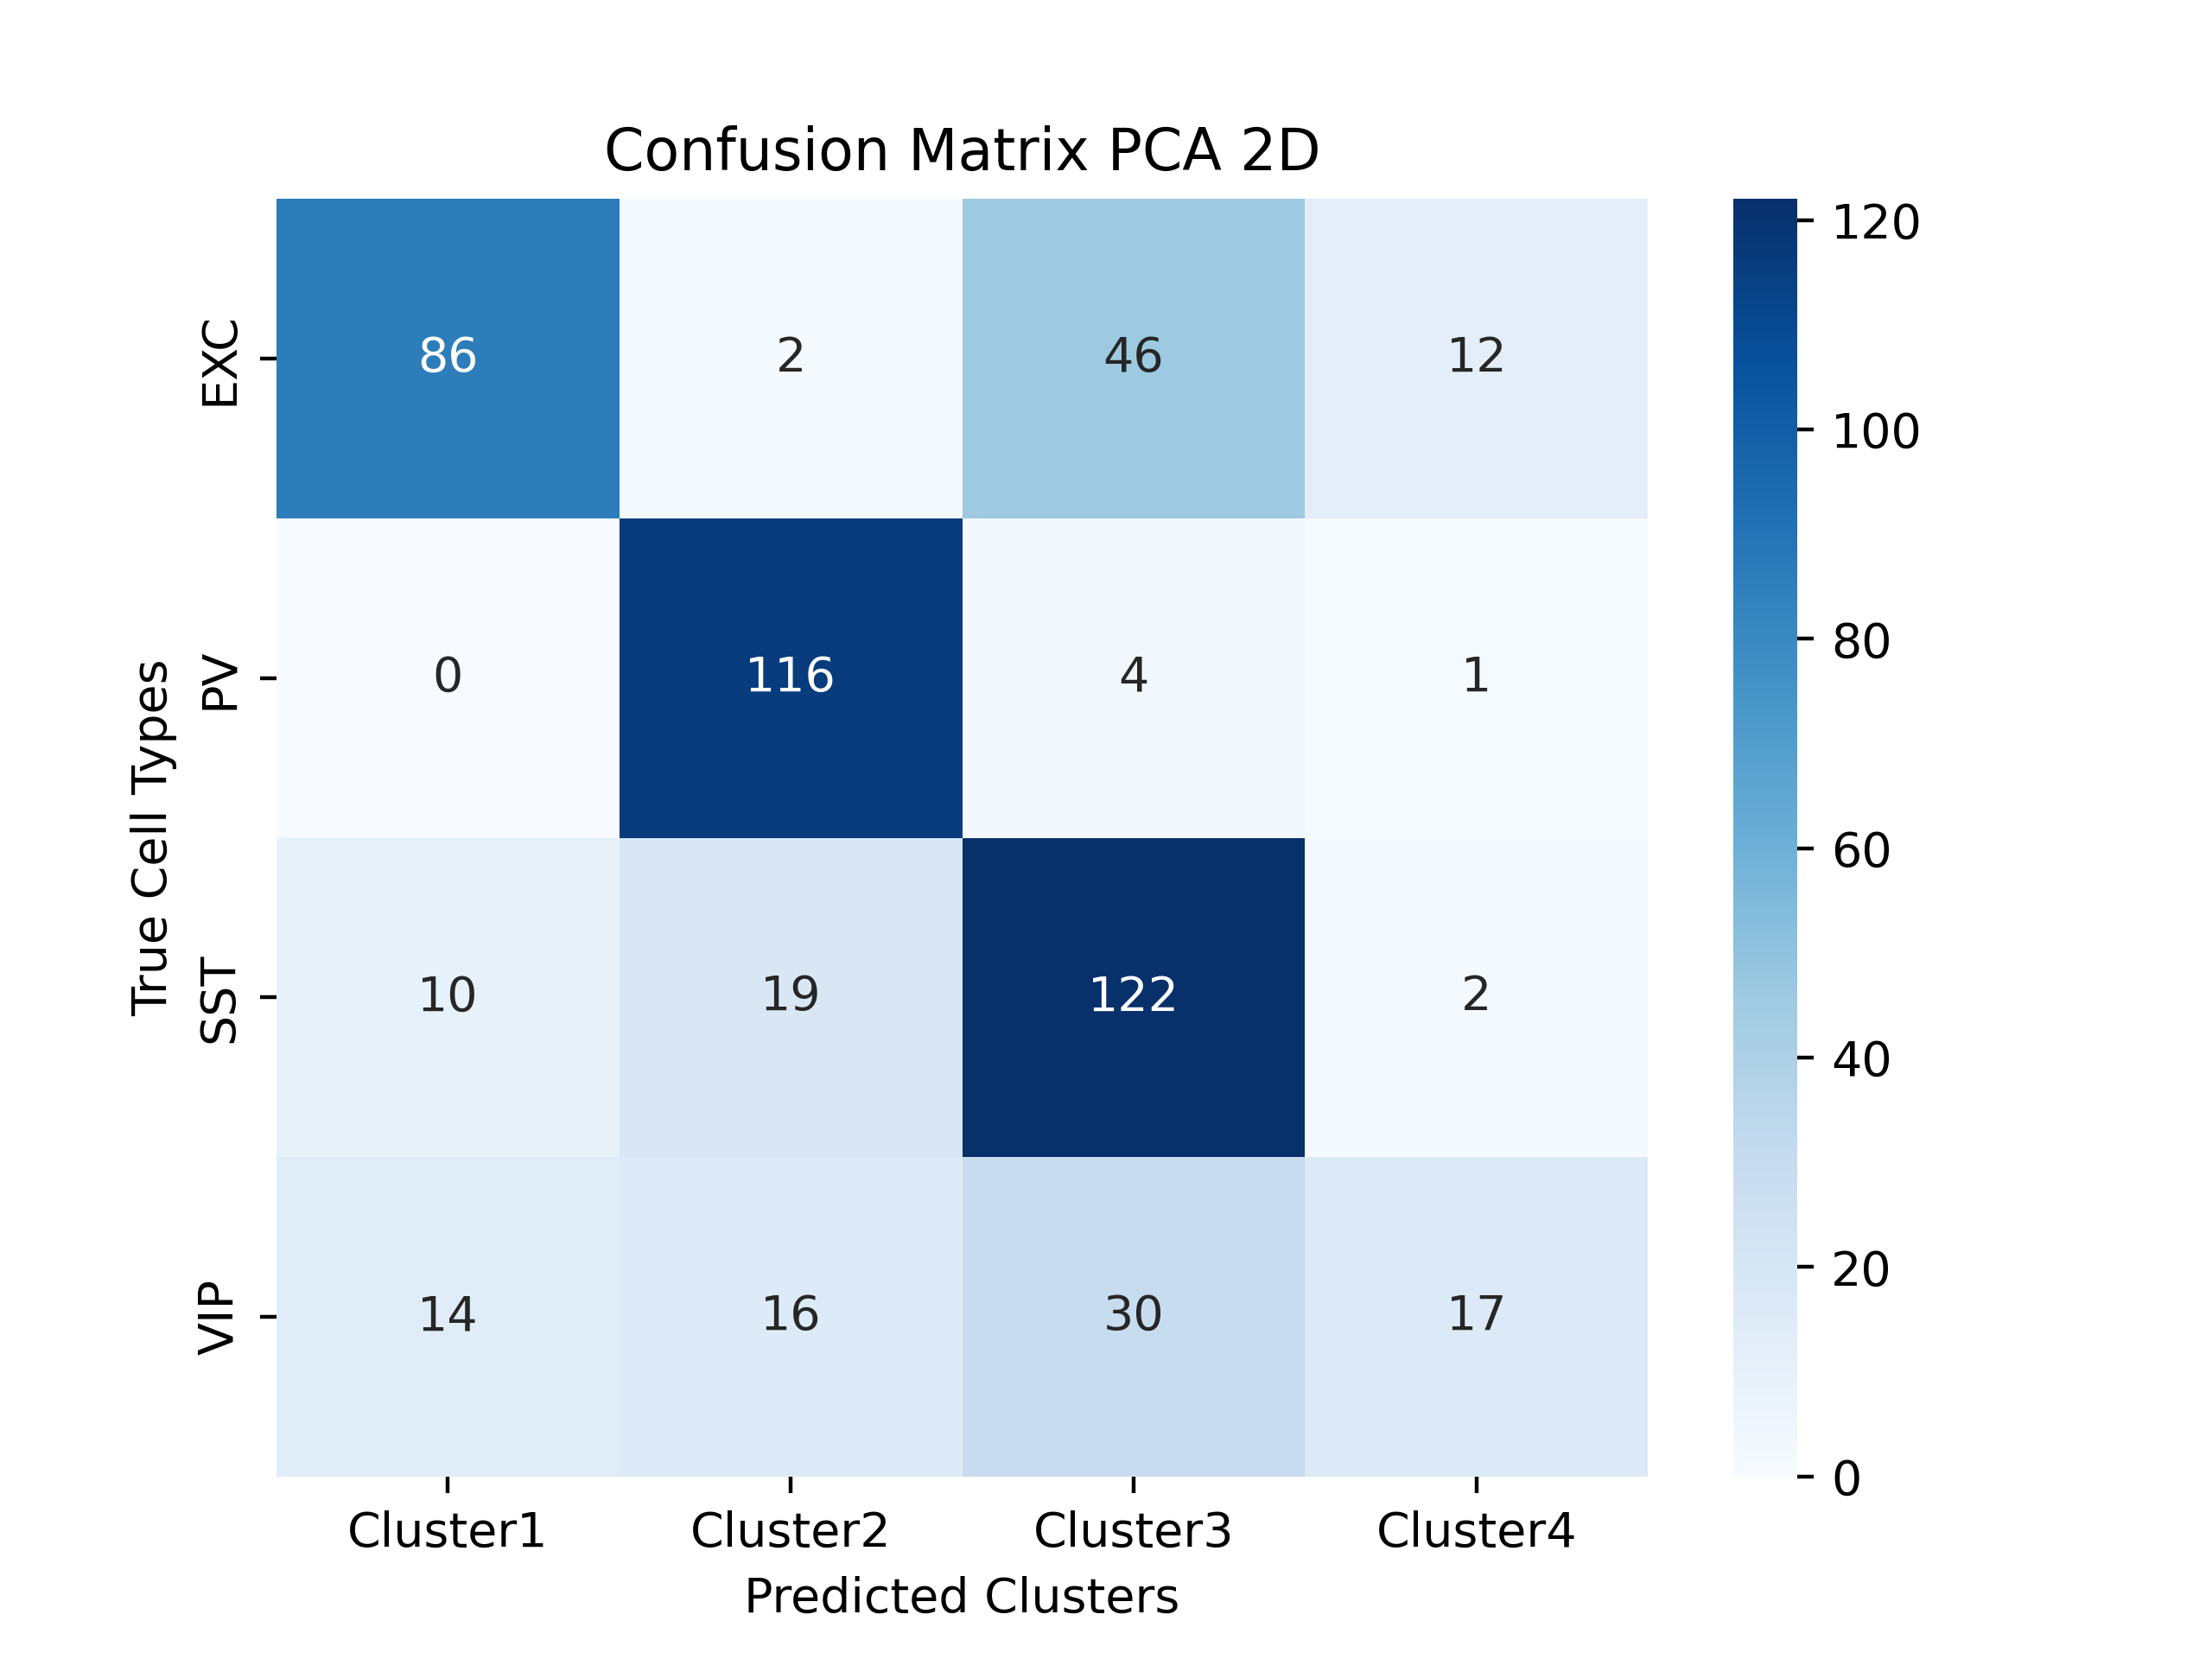
\includegraphics[width=0.5\columnwidth]{figures/Confusion Matrix PCA 2D.png}
%   \caption{}
%   \label{fig:cfm_pca2D_wrapped}
% \end{wrapfigure}


% Example on how to add sub-captions
% \begin{figure}%
%   \centering
%   \subfloat[Confusion Matrix PCA 2D]{{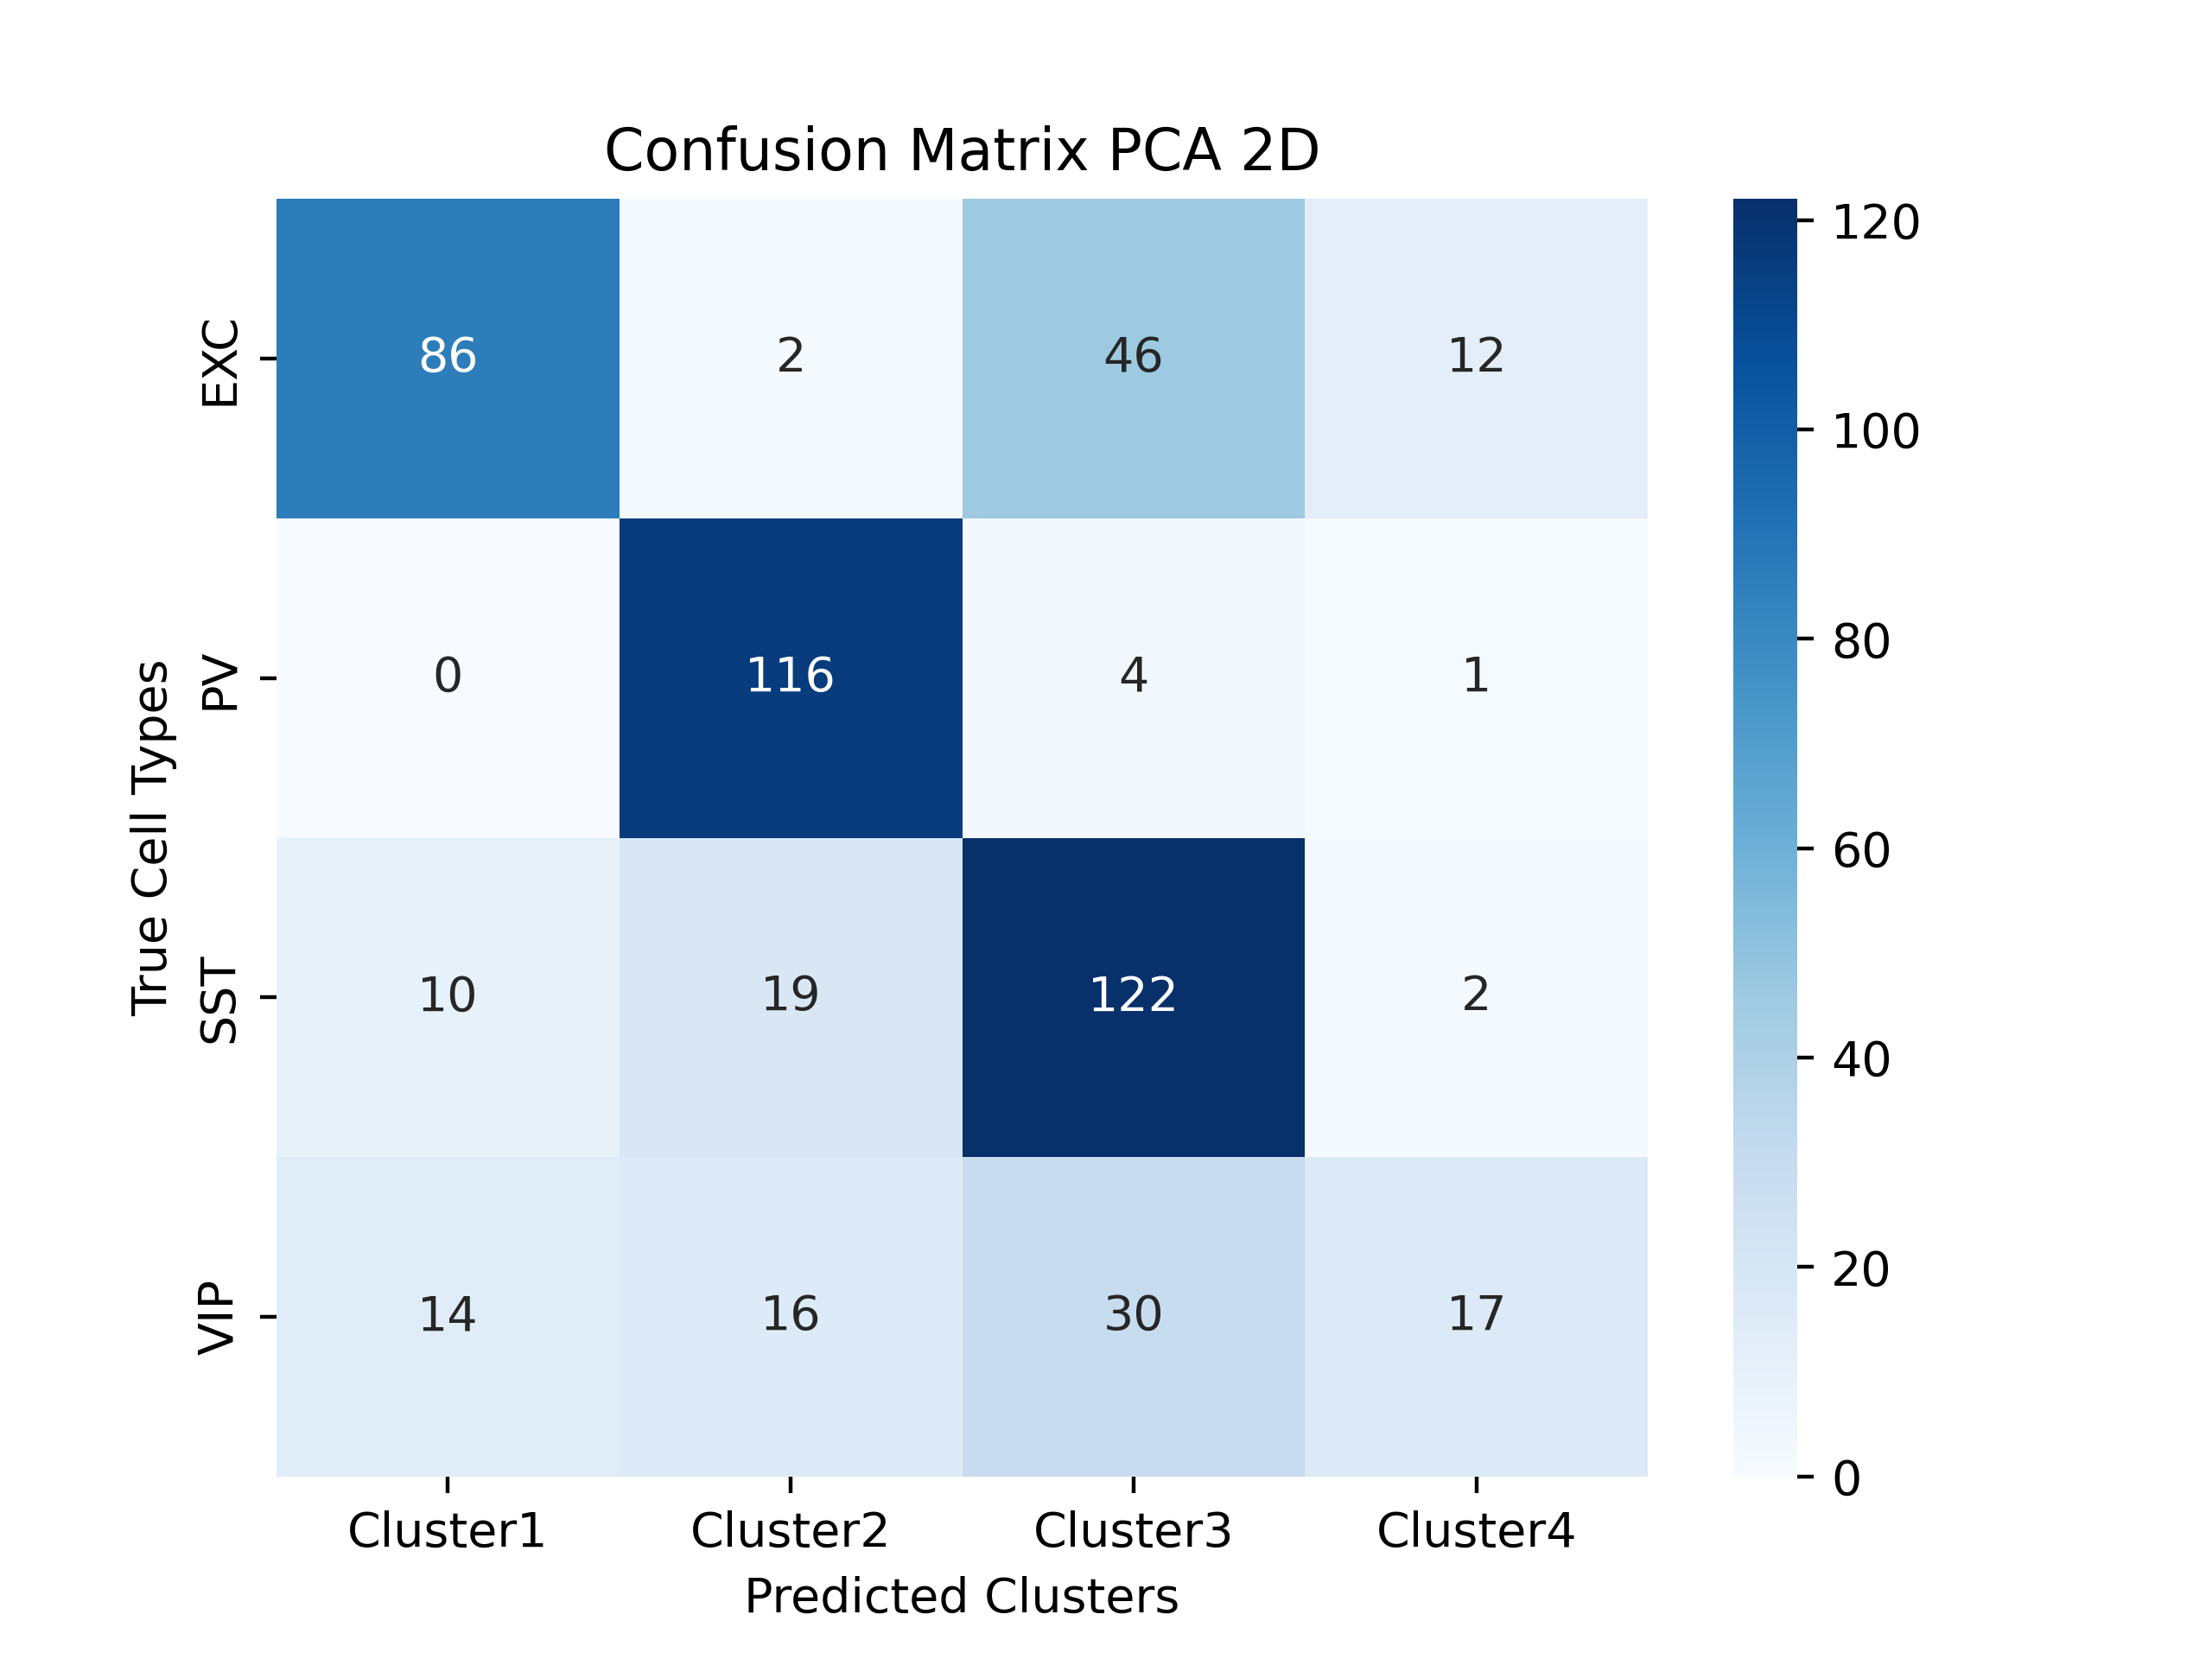
\includegraphics[width=4cm]{figures/Confusion Matrix PCA 2D.png} }}%
%   % \qquad
%   \subfloat[Confusion Matrix PCA 3D]{{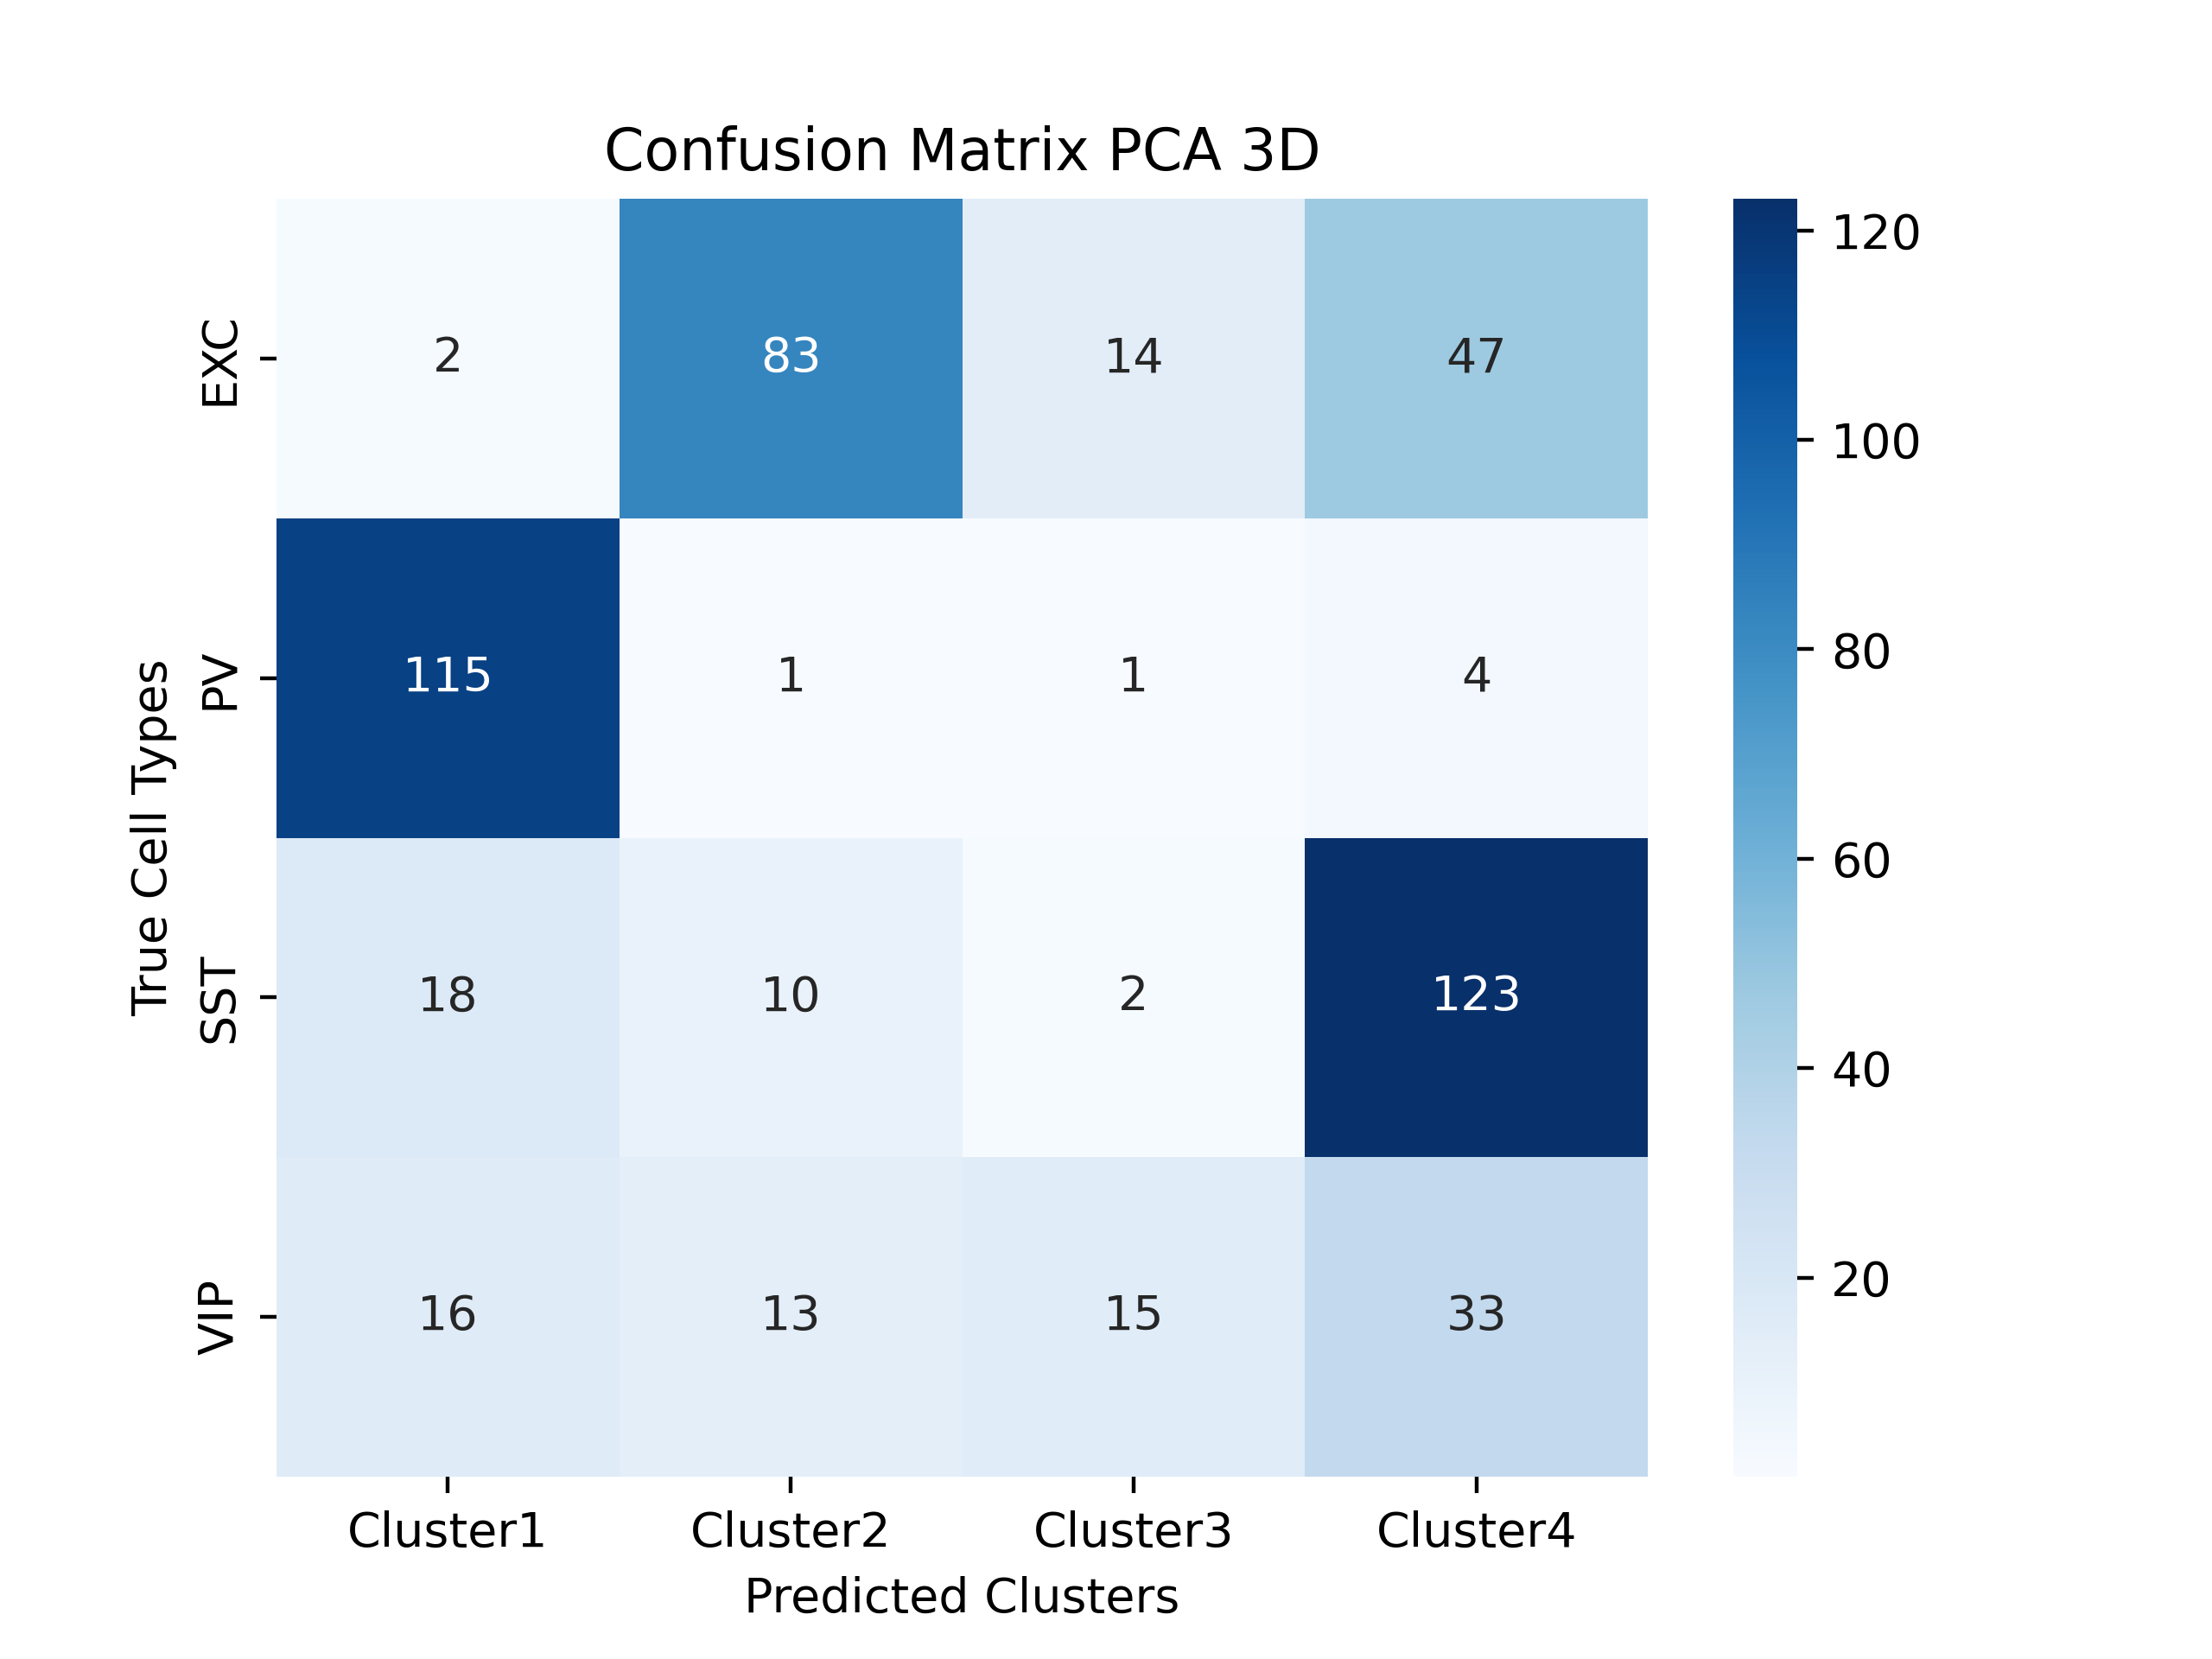
\includegraphics[width=4cm]{figures/Confusion Matrix PCA 3D.png} }}%
%   \caption{2 Figures side by side}%
%   \label{fig:example}
% \end{figure}




The mean firing rate of neurons is intricately linked to properties such as the action potential (AP) threshold, mean membrane potential (Vm), and standard deviation (SD) of Vm. Our analyses revealed interesting patterns in these relationships.

Our findings suggest that the firing rate exhibits a significant correlation with the mean Vm, and to a lesser extent, with the standard deviation of Vm. However, no clear correlation was observed with the AP threshold across all cell classes.

Additionally, for all cell classes, we observed a significant linear correlation between the change in firing rate and the change in Vm at whisking onset. Notably, there was a significant positive correlation between the change in Vm and firing rate at the onset of whisking, particularly with the depth of SST neurons.

Identification of Influencing Properties on Mean Firing Rate

From figure X, it becomes evident that certain properties exert a more pronounced impact on the mean firing rate of cortical neurons across cell classes.

In line with our course knowledge:

The lower the AP threshold, the higher the firing rate. However, this relationship does not hold uniformly across all cell classes.

A higher mean Vm generally corresponds to a lower firing rate, consistent with established principles.

Contrary to the general trend, our analyses did not reveal a clear correlation between AP threshold and firing rate for all cell classes. This suggests nuanced interactions that go beyond the conventional understanding.

In conclusion, the intricate interplay of AP threshold, mean Vm, and SD of Vm varies across cell classes. The nuanced relationships discovered in our analyses provide valuable insights into the factors influencing the mean firing rate of cortical neurons.


\subsection{Question 2}
Question 2 (2/10 marks):
\begin{enumerate}
  \item What are the specificities of each class of cortical neurons allowing to best distinguish excitatory vs inhibitory neurons?
  \item And between the different subclasses of inhibitory neurons?
  \item Justify your answers with some graphs.
\end{enumerate}


Our investigation into the distinct characteristics of cortical neurons aims to unravel the subtle nuances that facilitate the discrimination between excitatory and inhibitory neurons, as well as the differentiation among inhibitory neuron subclasses. The delineation below provides a concise summary of our findings, supported by pertinent graphs.

\subsubsection{Excitatory Neurons}
Excitatory neurons consistently display low action potential (AP) firing rates. Their membrane potential (Vm) tends to be hyperpolarized compared to inhibitory neurons. At the onset of whisking, excitatory neurons depolarize, possibly due to increased excitatory input from the thalamus. Following whisking onset, a transient hyperpolarization occurs, demanding further investigation. Prolonged whisking is associated with reduced fluctuations in slow frequencies of Vm dynamics. Individual neurons exhibit Vm dynamics synchronized with the whisking cycle. Active touch induces robust depolarization with a slight increase in firing rate. Excitatory neurons exhibit depressing postsynaptic potential (PSP) responses during high-frequency palpation, accompanied by a reliable peak Vm.

\subsubsection{PV-expressing GABAergic Neurons}
PV neurons stand out with notably higher firing rates compared to other neuronal classes. Elevated firing rates are likely driven by robust excitatory synaptic input from nearby excitatory neurons and the thalamus. At the onset of whisking, PV neurons depolarize, with a more pronounced increase in firing rate in deeper neurons. Similar to excitatory neurons, PV neurons undergo depolarization with reduced slow Vm fluctuations during prolonged whisking. They exhibit prominent whisking phase-locked Vm dynamics. Active touch induces significant and rapid depolarization, accompanied by a strong increase in AP firing. Touch-evoked responses are suppressed at short intercontact intervals.

\subsubsection{VIP-expressing GABAergic Neurons}
VIP neurons share an AP waveform duration similar to excitatory neurons, posing a challenge for identification in unidentified neuron recordings. They depolarize and increase firing rate at the onset and during prolonged whisking. VIP neurons display late excitation during active touch, consistent with responses to passively applied whisker deflections. They exhibit modest whisking phase-locked Vm fluctuations. VIP neurons appear more influenced by overall behavioral state (whisking vs. quiet) than specific aspects of whisker sensory processing.

\subsubsection{SST-expressing GABAergic Neurons}
SST neurons feature significantly smaller amplitude slow Vm fluctuations compared to other classes. On average, SST neurons hyperpolarize at the onset and during prolonged whisking. They display a distinctive relationship to intercontact intervals, exhibiting a small hyperpolarization at long intervals and excitatory PSP responses at short intervals. SST neurons exhibit relatively weak active touch responses, aligning with near-absent AP responses evoked by passive whisker stimulation.


\subsection{Question 3}
Question 3 (1/10 mark):

\begin{enumerate}
  \item Summarize what happens at whisking onset time and active-contact onset time for the different cell-classes. Justify your answers with some graphs.
\end{enumerate}





%-----------------------------------------------------


\section{Methods}

\begin{enumerate}
  \item Explain in a few lines what is the question you want to address, what is the rational, and what is your hypothesis? % TODO
  \item Explain briefly what analyses you have done to answer your question and how you have proceeded.
  \item Present your results with some graphs and explanations.
  \item Interpret your results, answer your question if possible or explain why you cannot, conclude.
\end{enumerate}

\subsection{Data Preprocessing}
\subsubsection{Predictors}

We decided to focus only on “free whisking” sweeps, which amounted to 497 different samples.
From these sweeps we decided to use as predictors the calculated firing rate (\textit{firing\_rate}), action potential (AP) threshold and duration (\textit{ap\_threshold} and \textit{ap\_duration}), the mean and the standard deviation of the membrane potential (\textit{mean\_vm} and \textit{std\_vm}), and spectral domain information in the form of the lowest and the highest Fourier amplitudes (\textit{fft\_low} and \textit{fft\_high}).
Whenever a sweep did not have an AP, we replaced both AP duration and threshold by a value of 0. In hindsight this is biologically nonsensical.
These seven features created a data matrix $X_1 \in \mathbb{R}^{497\times7}$ to be paired with the response variable $y \in \mathbb{R}^{497\times1}$ corresponding to each cell class.

\subsubsection{Additional Extracted features}
In addition to the 7 features mentioned above, the 13 features described in Table-\ref{tab:variables} were extracted and added from each sweep, widening our data size $X_2 \in \mathbb{R}^{497\times20}$.
One can observe the correlation between each variable present in $X_2$ in Annex (Fig. \ref{fig:correlation}). 

\subsubsection{Standardization}
For supervised learning, the $X_2 \in \mathbb{R}^{497\times20}$ data was used. When splitting, training data was standardized, and the same transformation was applied to the test data.
For unsupervised learning the $X_1 \in \mathbb{R}^{497\times7}$ data was used. It was standardized in its entirety prior to dimensionality reduction.

\begin{table}[h!]
  \centering
  \begin{tabular}{|l|p{0.6\linewidth}|}
  \hline
  \textbf{Variable} & \textbf{Description} \\
  \hline
  \textit{ap\_amp\_mean} & Average action potential amplitude for each sweep; any missing values or NaNs were replaced with 0. \\
  \hline
  \textit{ap\_amp\_cv} & Coefficient of variation (= std / mean) of the action potential amplitudes for each sweep; any missing values or NaNs were replaced with 0. \\
  \hline
  \textit{mean\_ap\_upstroke} & Average maximal rate of increase of the membrane potential during the action potential upstroke; any missing values or NaNs were replaced with 0. \\
  \hline
  \textit{ap\_upstroke\_cv} & Coefficient of variation of the maximal rate of increase of the membrane potential during the action potential upstroke; any missing values or NaNs were replaced with 0. \\
  \hline
  \textit{mean\_ap\_downstroke} & Average maximal rate of decrease of the membrane potential during the action potential downstroke; any missing values or NaNs were replaced with 0. \\
  \hline
  \textit{ap\_downstroke\_cv} & Coefficient of variation of the maximal rate of decrease of the membrane potential during the action potential downstroke; any missing values or NaNs were replaced with 0. \\
  \hline
  \textit{isi\_mean} & Average duration between consecutive action potentials (inter-spike intervals); any missing values or NaNs were replaced with 50. \\
  \hline
  \textit{isi\_cv} & Coefficient of variation of the duration between consecutive action potentials; any missing values or NaNs were replaced with 0. \\
  \hline
  \textit{irregularity\_index} & Index indicating how regular the inter-spike intervals are, i.e., the mean of the difference between the durations of consecutive ISIs; any missing values or NaNs were replaced with 0. \\
  \hline
  \textit{adaptation\_index} & Another index indicating how regular the inter-spike intervals are; equal to the sum of the durations of consecutive ISIs divided by their difference. It is zero for a constant firing rate, negative for an increasing firing rate, and positive for a decreasing firing rate; any missing values or NaNs were replaced with 0, and very large values were capped to $10^{10}$. \\
  \hline
  \textit{nb\_bursts} & Number of bursts per sweep. Two consecutive action potentials are considered part of the same burst if the duration between them is less than 10ms; any missing values or NaNs were replaced with 0. \\
  \hline
  \textit{mean\_burst\_dur} & Mean duration of bursts; any missing values or NaNs were replaced with 0. \\
  \hline
  \textit{burst\_dur\_cv} & Coefficient of variation of the duration of bursts; any missing values or NaNs were replaced with 0. \\
  \hline
  \end{tabular}
  \caption{Description of Added Variables}
  \label{tab:variables}
\end{table}


\subsection{Supervised Learning}

\subsubsection{Models}
In this study, a range of established machine learning algorithms available in the \textit{Sci-kit Learn} library \cite{scikit-learn} were tested. These are Logistic Regression, Random Forest, Gradient Boosting, AdaBoost, Decision Tree, Support Vector Machines, and a Gaussian Naive Bayes.
Despite their effectiveness, deep learning models were not implemented as they would be hard to interpret.

\subsubsection{Evaluation Metric}
In order to get an estimate of the performance of each model on unseen data, we opted for a stratified 5-fold Cross Validation (CV) -which retains the original distribution when splitting the data- paired with the multi-class $F1$ score as an evaluation metric. This metric calculates the $F1$ score ``for each label, and finds their average weighted by support (the number of true instances for each label)." \cite{scikit-learn} It therefore takes into account multi-class imbalance which was prevalent in our data (much more EXC or SST cells than VIP cells).

\subsubsection{Hyperparameter Optimization (HPO)}
Hyperparameters (HP) of a model were tuned using a Bayesian optimization algorithm available in the \textit{Scikit-Optimize} library \cite{scikit-optimize}, in order to maximise the stratified 5-fold CV $F1$ score.

\subsubsection{Feature Importance}
The (HPO) models that achieved the best test score were trained on the entire data, and each individual feature importance was assessed using a metric specific to the type of classifier used. For tree-based ensemble methods (Gradient Boosting or Random Forest), the default feature importance attribute was used. It is computed as the mean and standard deviation of accumulation of the impurity decrease within each tree. For linear models utilizing weights (Linear SVC and Logistic Regression), the mean absolute weights across each class was used.

\subsubsection{Ensembling}
After having found the top models, we wanted to see whether combining their predictions would yield a higher result. As such, a final ``ensemble" voting classifier with a majority voting rule was created and evaluated.

\subsection{Unsupervised Learning}

\subsubsection{Dimensionality Reduction}
Dimensionality reduction techniques were employed in order to visualize the data in lower dimensional sub-spaces (2D and 3D). Hence, we would be able to visualize whether there is a spatial arrangement between each cell class. The three employed techniques were Principal Component Analysis (PCA), t-distributed Stochastic Neighbor Embedding (t-SNE), and Uniform Manifold Approximation and Projection (UMAP).

\subsubsection{K-Means Clustering}
K-Means clustering algorithm was used in the lower dimensional subspace projections of our data. We fixed K to be equal to the number of cell classes present ($K=4$), in order to determine whether each cluster could represent a specific cell class.

%-----------------------------------------------------

\section{Results}

\subsection{Best Models}

\begin{figure}[h!]
  \centering
  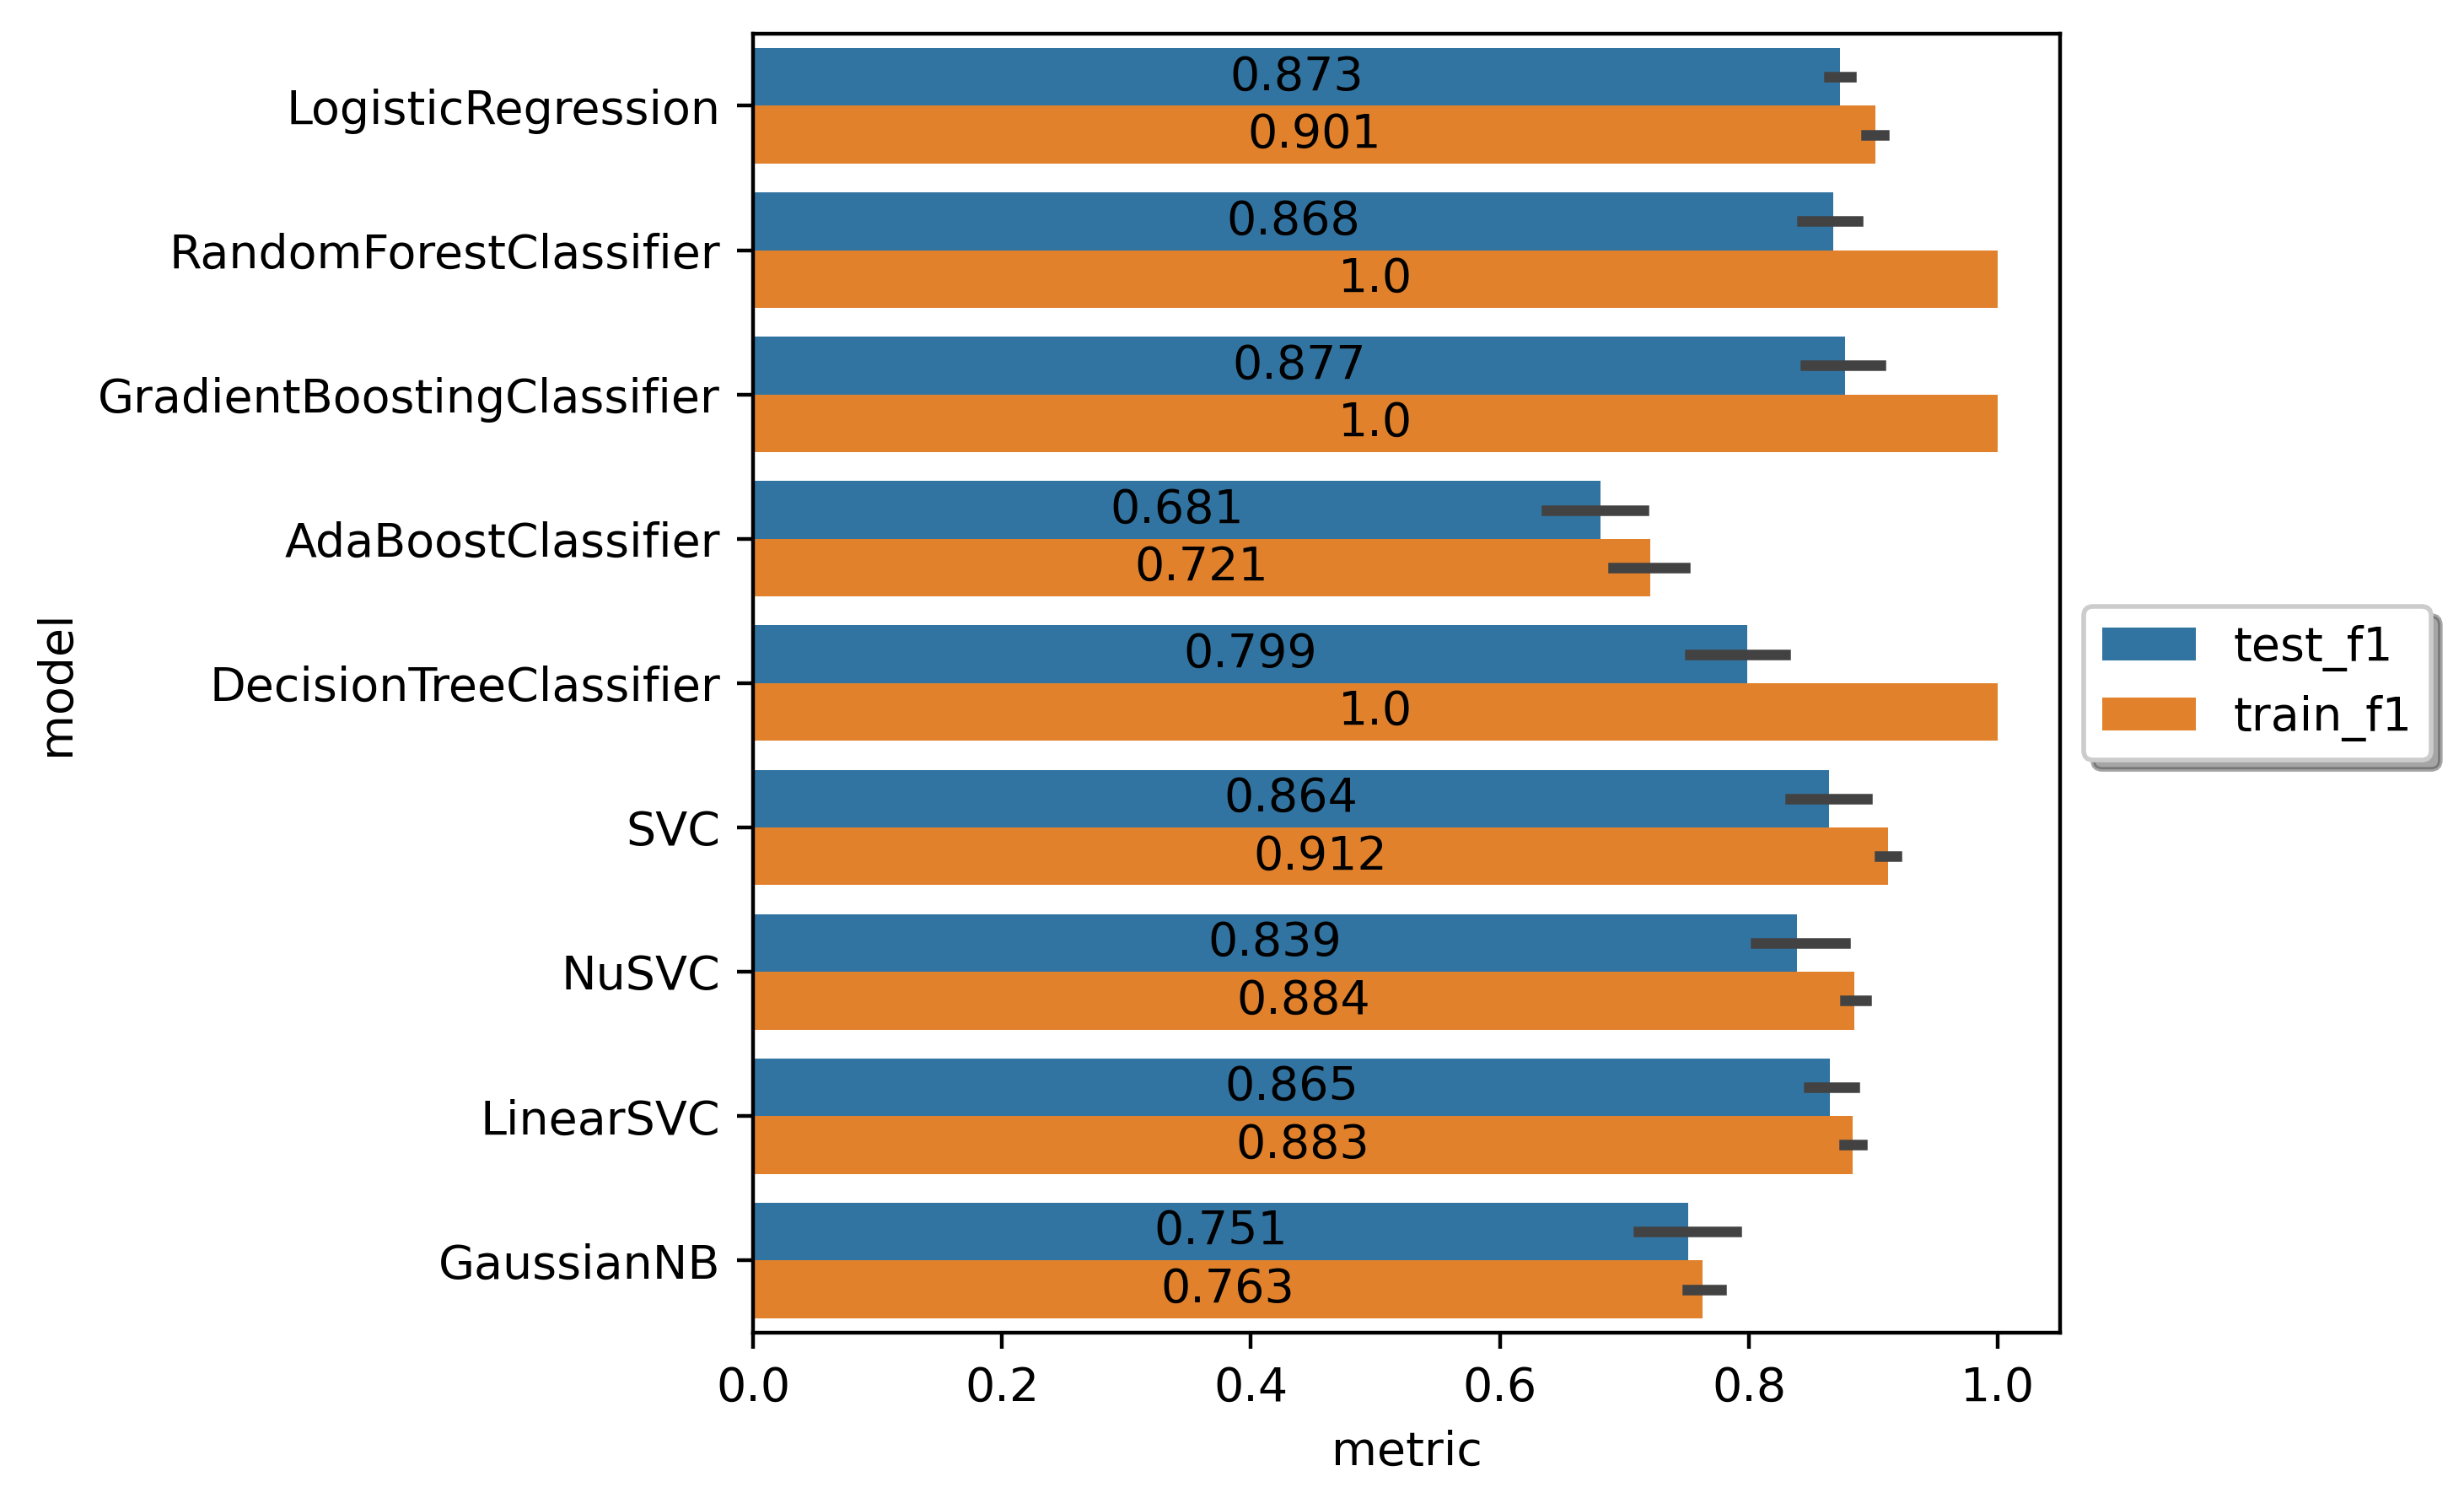
\includegraphics[width=\columnwidth]{figures/models_unturned_f1.png}
  \caption{F1 score performances, on a stratified 5-Fold CV, for a range of models tested.}
  \label{fig:models_untuned}
\end{figure}

\begin{table}[h!]
  \centering
  \begin{tabular}{|l|l|l|l|}
  \hline
  \textbf{Model} & \textbf{Inference} & \textbf{Mean} & \textbf{Std} \\
  \hline
  Gradient Boosting & Test & 0.8888 & 0.0366 \\
   & Train & 1.0 & 0.0 \\
  \hline
  Linear Support Vector Machine & Test & 0.8832 & 0.0090 \\
   & Train & 0.9094 & 0.0125 \\
  \hline
  Random Forest & Test & 0.8789 & 0.0334 \\
   & Train & 1.0 & 0.0 \\
  \hline
  Logistic Regression & Test & 0.8756 & 0.0188 \\
   & Train & 0.9166 & 0.0136 \\
  \hline
  Ensemble & Test & 0.9065 & 0.0206 \\
   & Train & 0.9631 & 0.0072 \\
  \hline
  \end{tabular}
  \caption{Stratified 5-fold CV F1 score performance of top 4 best (HPO) models, plus the ensemble combination of them.}
  \label{tab:best_model_scores}
\end{table}

From Fig. \ref{fig:models_untuned} we can see that the four best unoptimized models, based on test performance, are: 1st GradientBoosting with a score of $0.877$, 2nd Logistic Regression, 3rd Random Forest and 4th Linear SVC. After having done HPO (Table-\ref{tab:best_model_scores}), these models improve by about 1 to 2 \%, every model in now above $0.8756$, and Linear SVC and Logistic Regression swap places. Furthermore, by ensembling these four best models, it is possible to increase test performance by an additional  1.77 \% (from $0.8888 \pm 0.0366$ to $0.9065 \pm 0.0206$).
It is interesting to notice that tree-based methods (Gradient Boosting and Random Forest) overfit to a greater extent, and have a higher standard deviation than linear models.

\begin{figure}[h!]
  \centering
  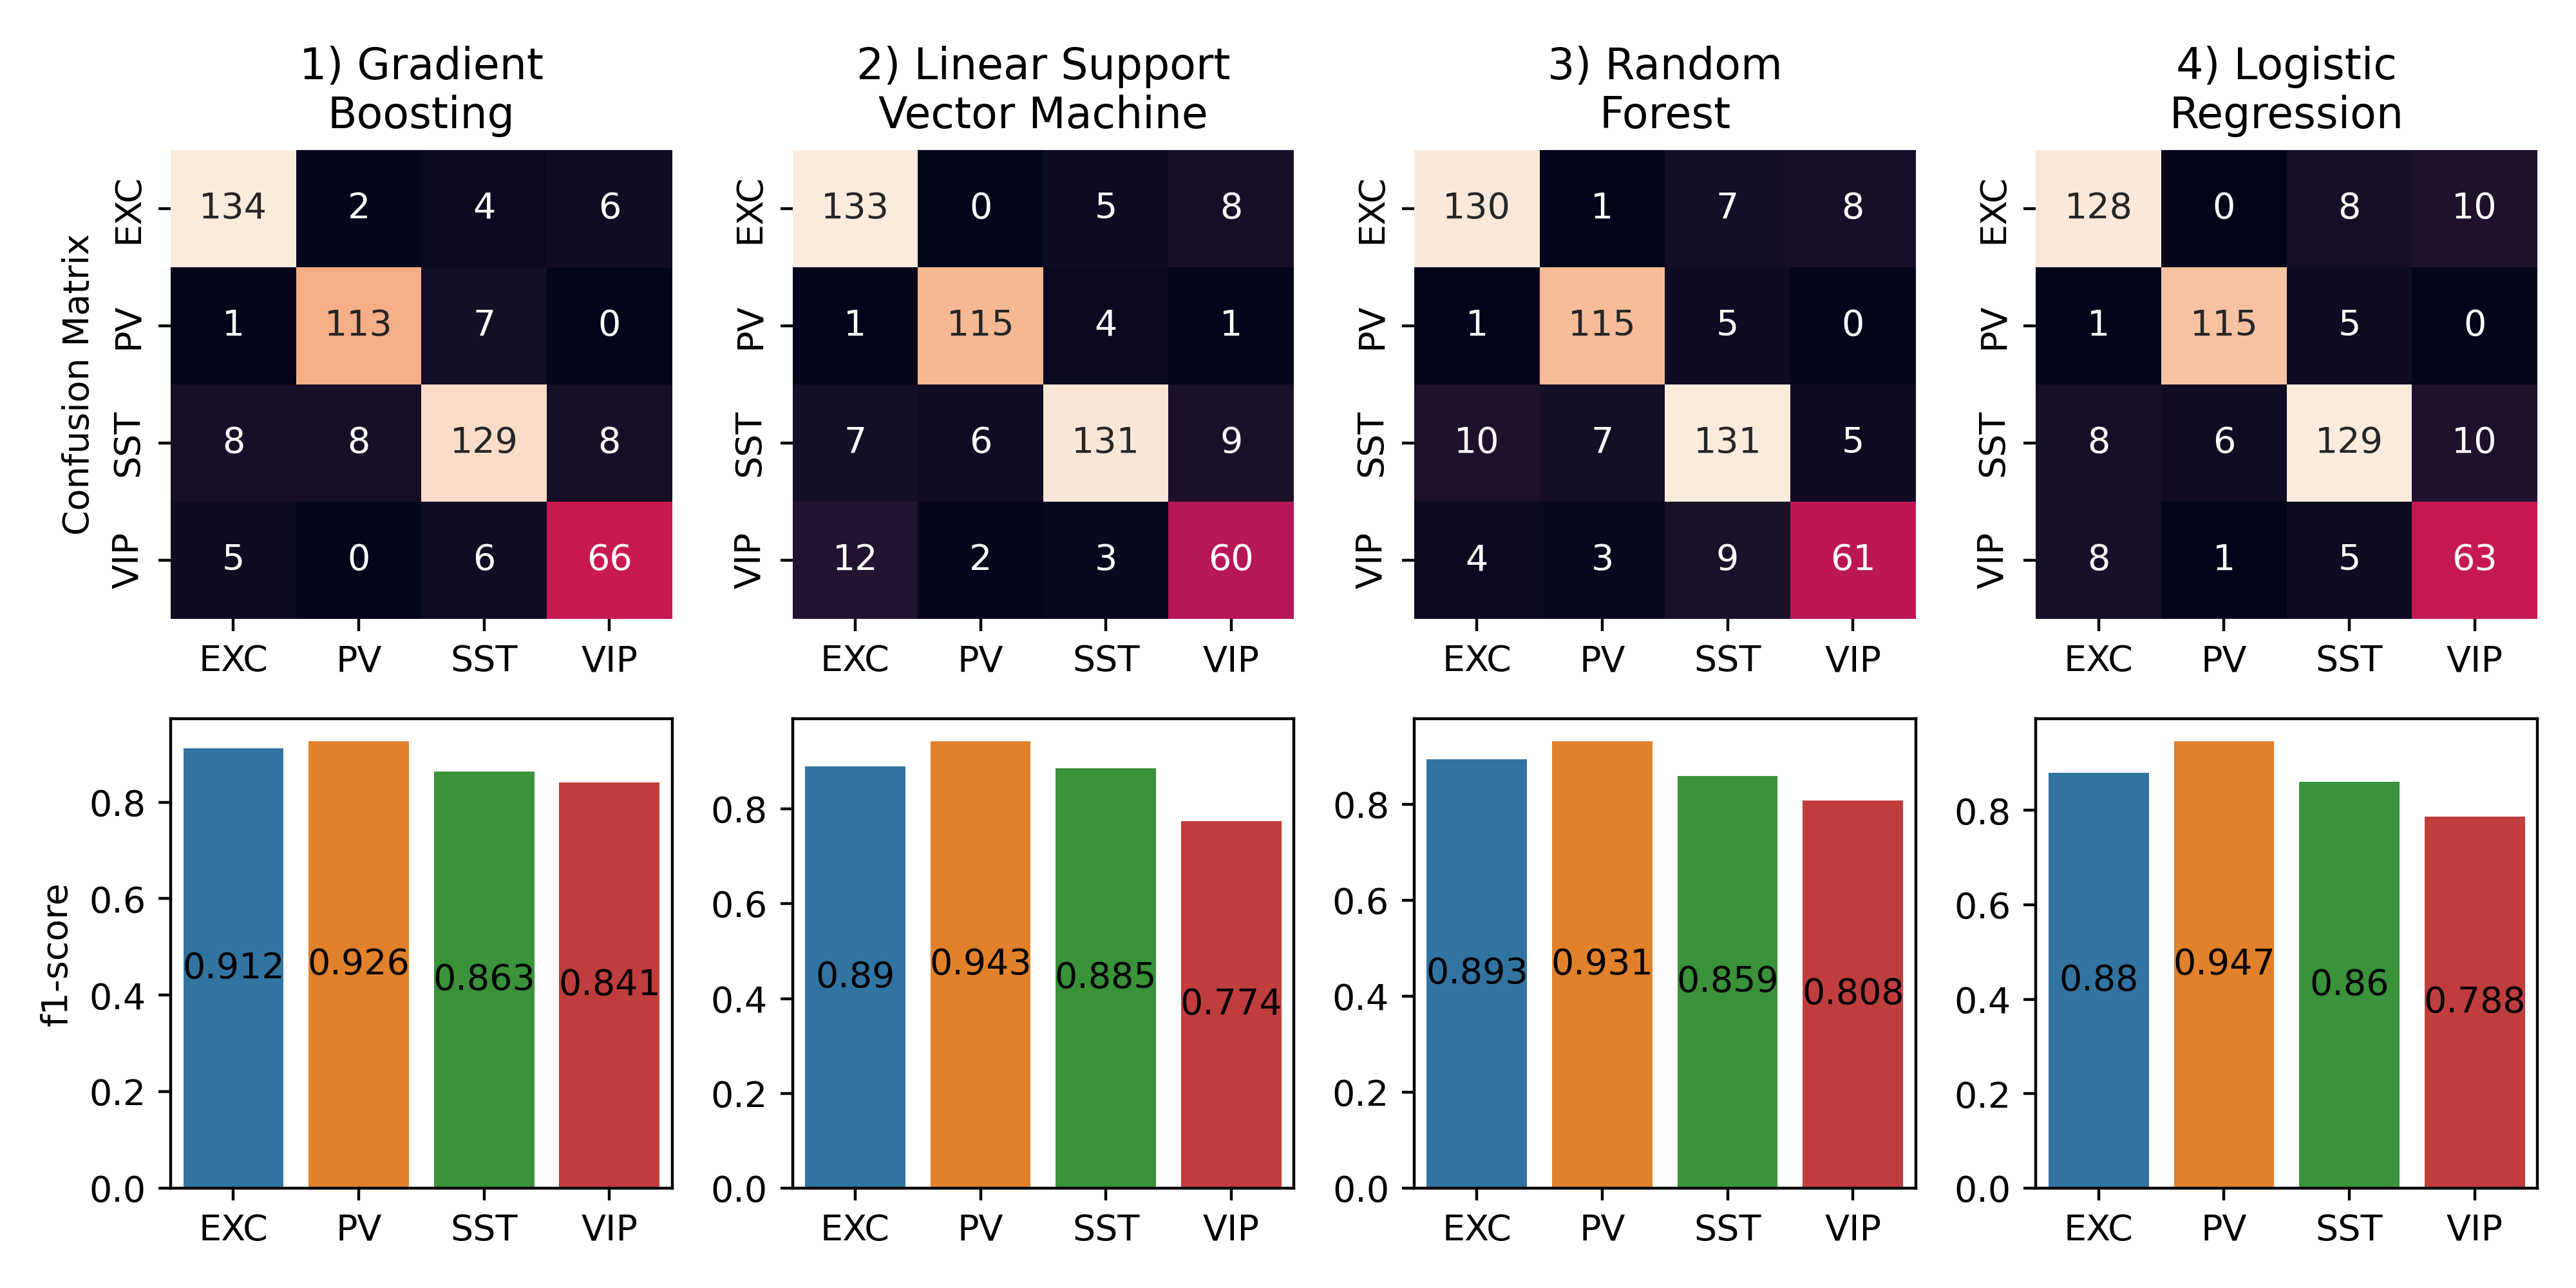
\includegraphics[width=\columnwidth]{figures/confusion_matrices_of_classifiers.png}
  \caption{Top 4 best model performances. Each column correspond to a model. Top row are confusion matrices based on a 5-Fold Stratified CV prediction. For each one of them the x-axis corresponds to predictions and the y-axis to the ground truth. Bottom row are the F1 scores for each cell type, calculated with the same prediction.}
  \label{fig:supervised_confusion_matrices}
\end{figure}

From Fig. \ref{fig:supervised_confusion_matrices}, 


\subsection{Feature Importance}

\begin{figure*}[h!]
  \centering
  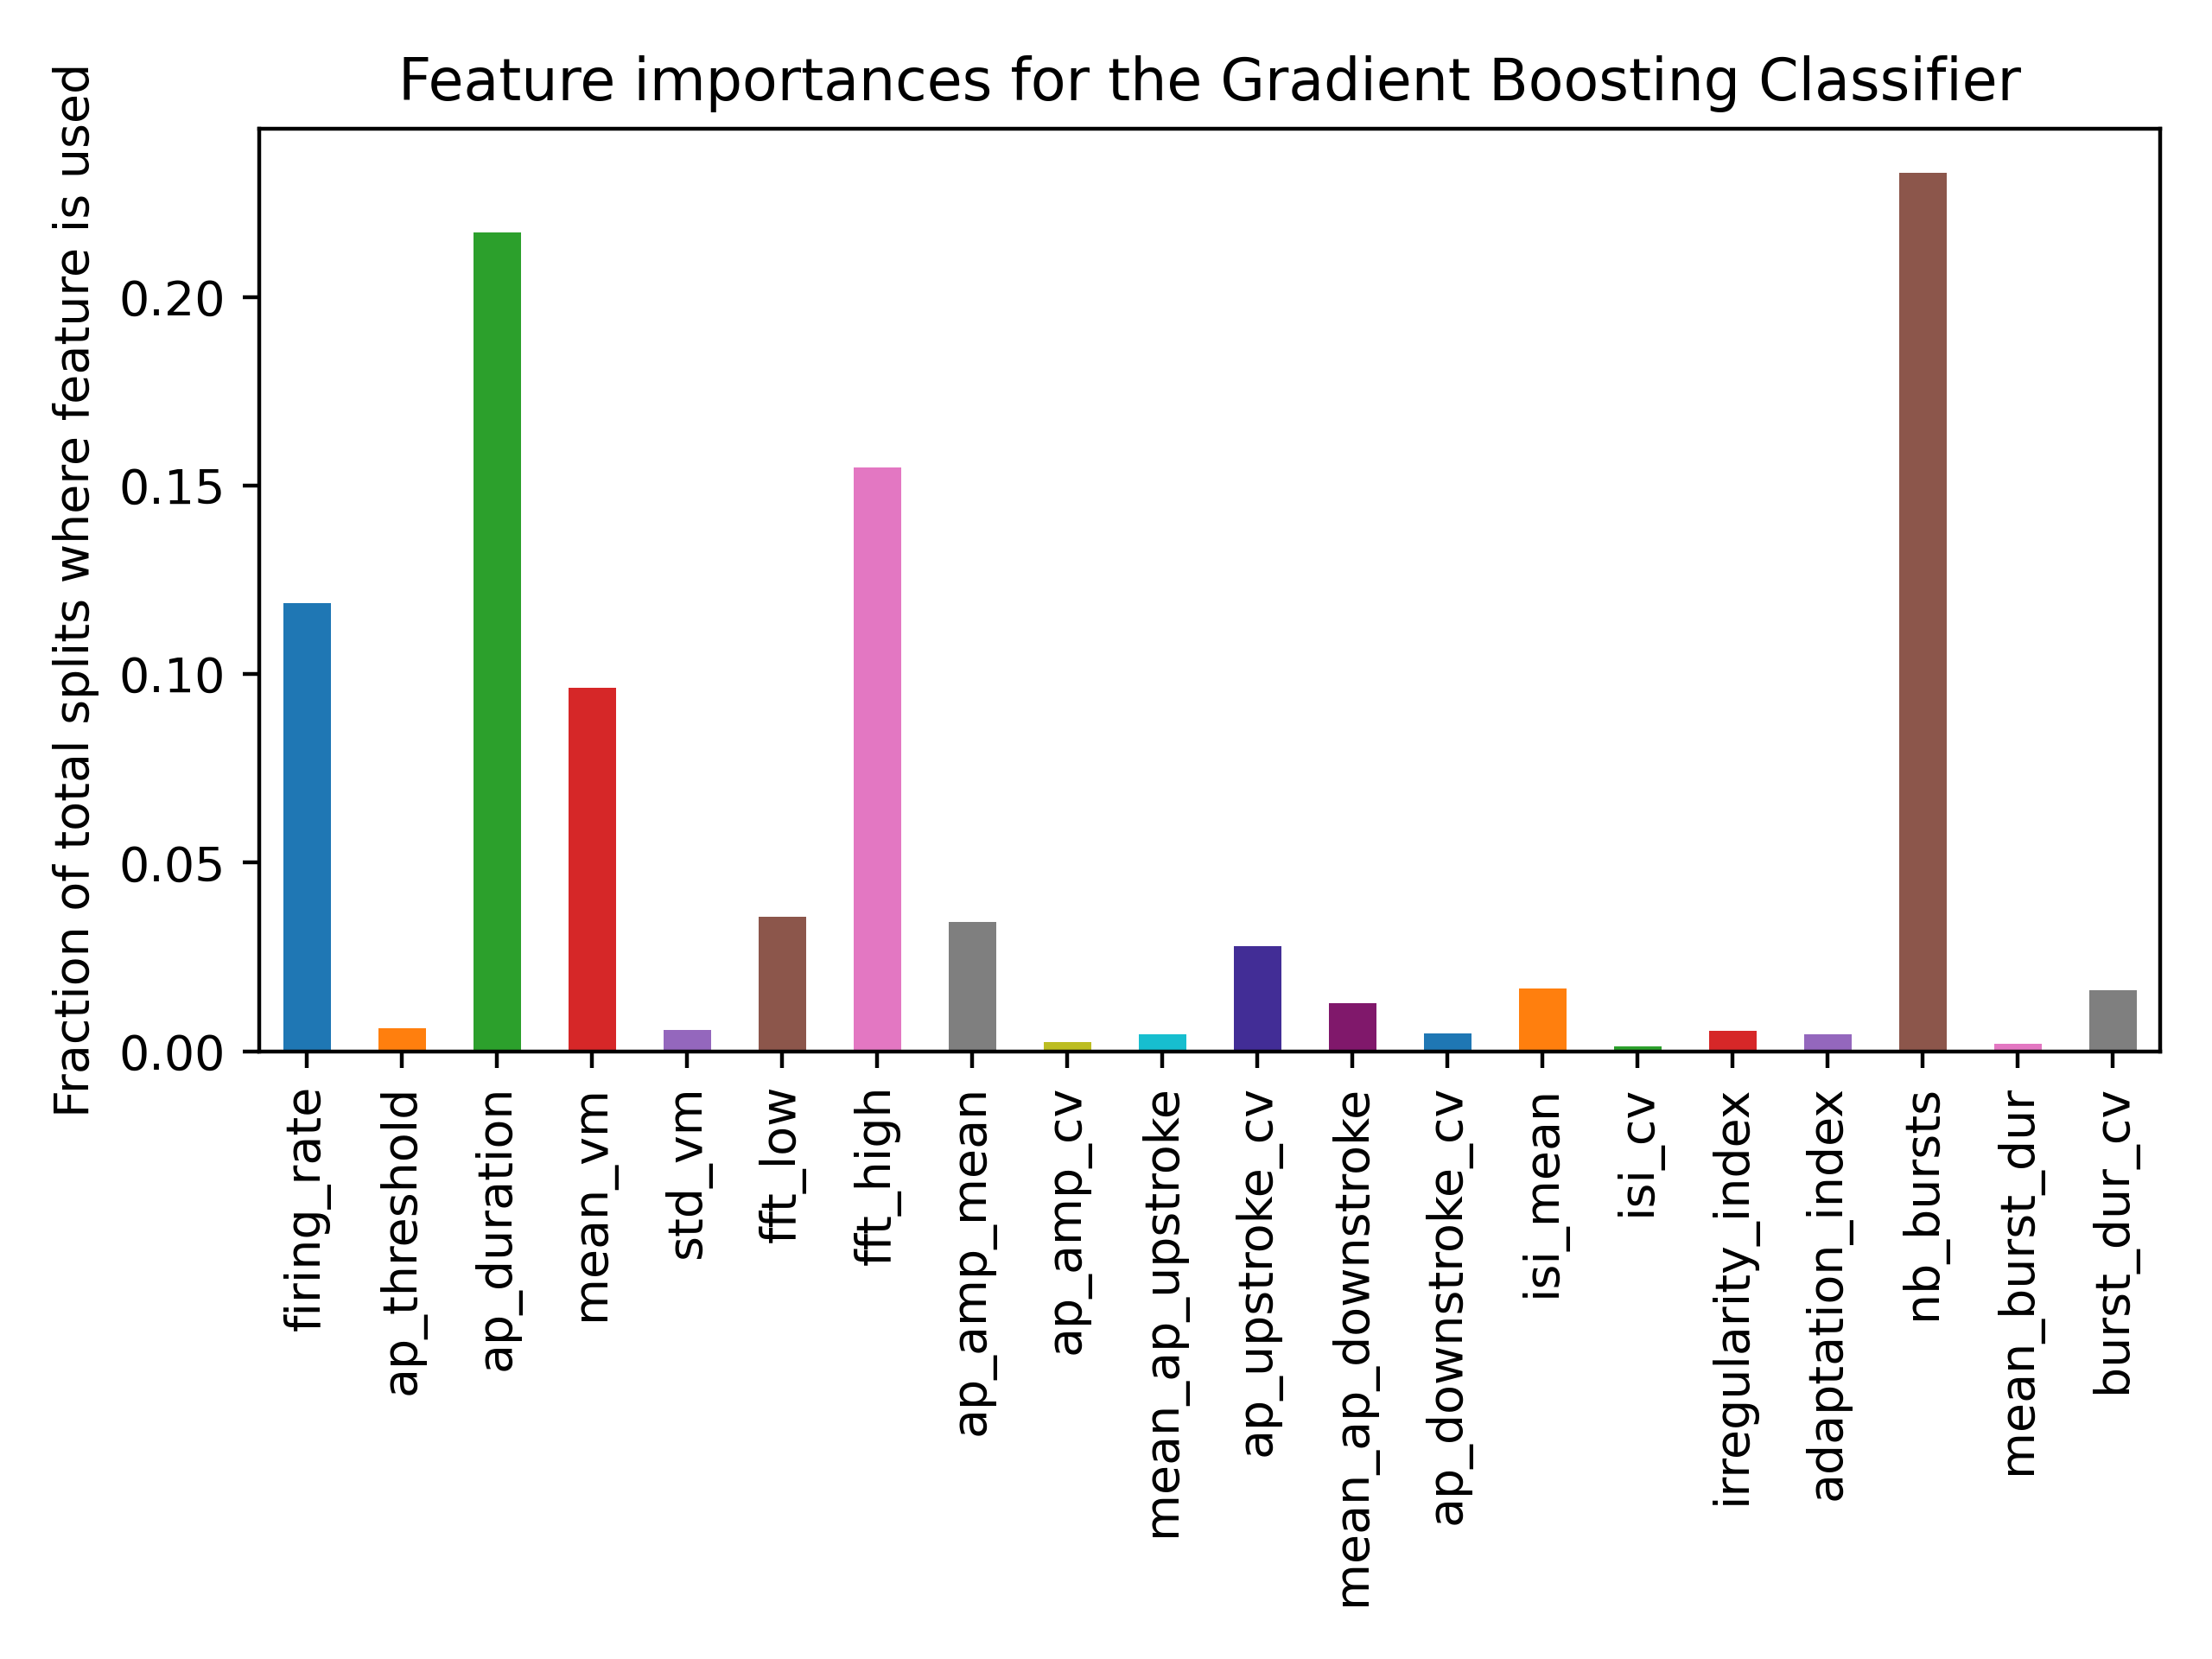
\includegraphics[width=0.9\columnwidth]{figures/feature_importance_gb.png}
  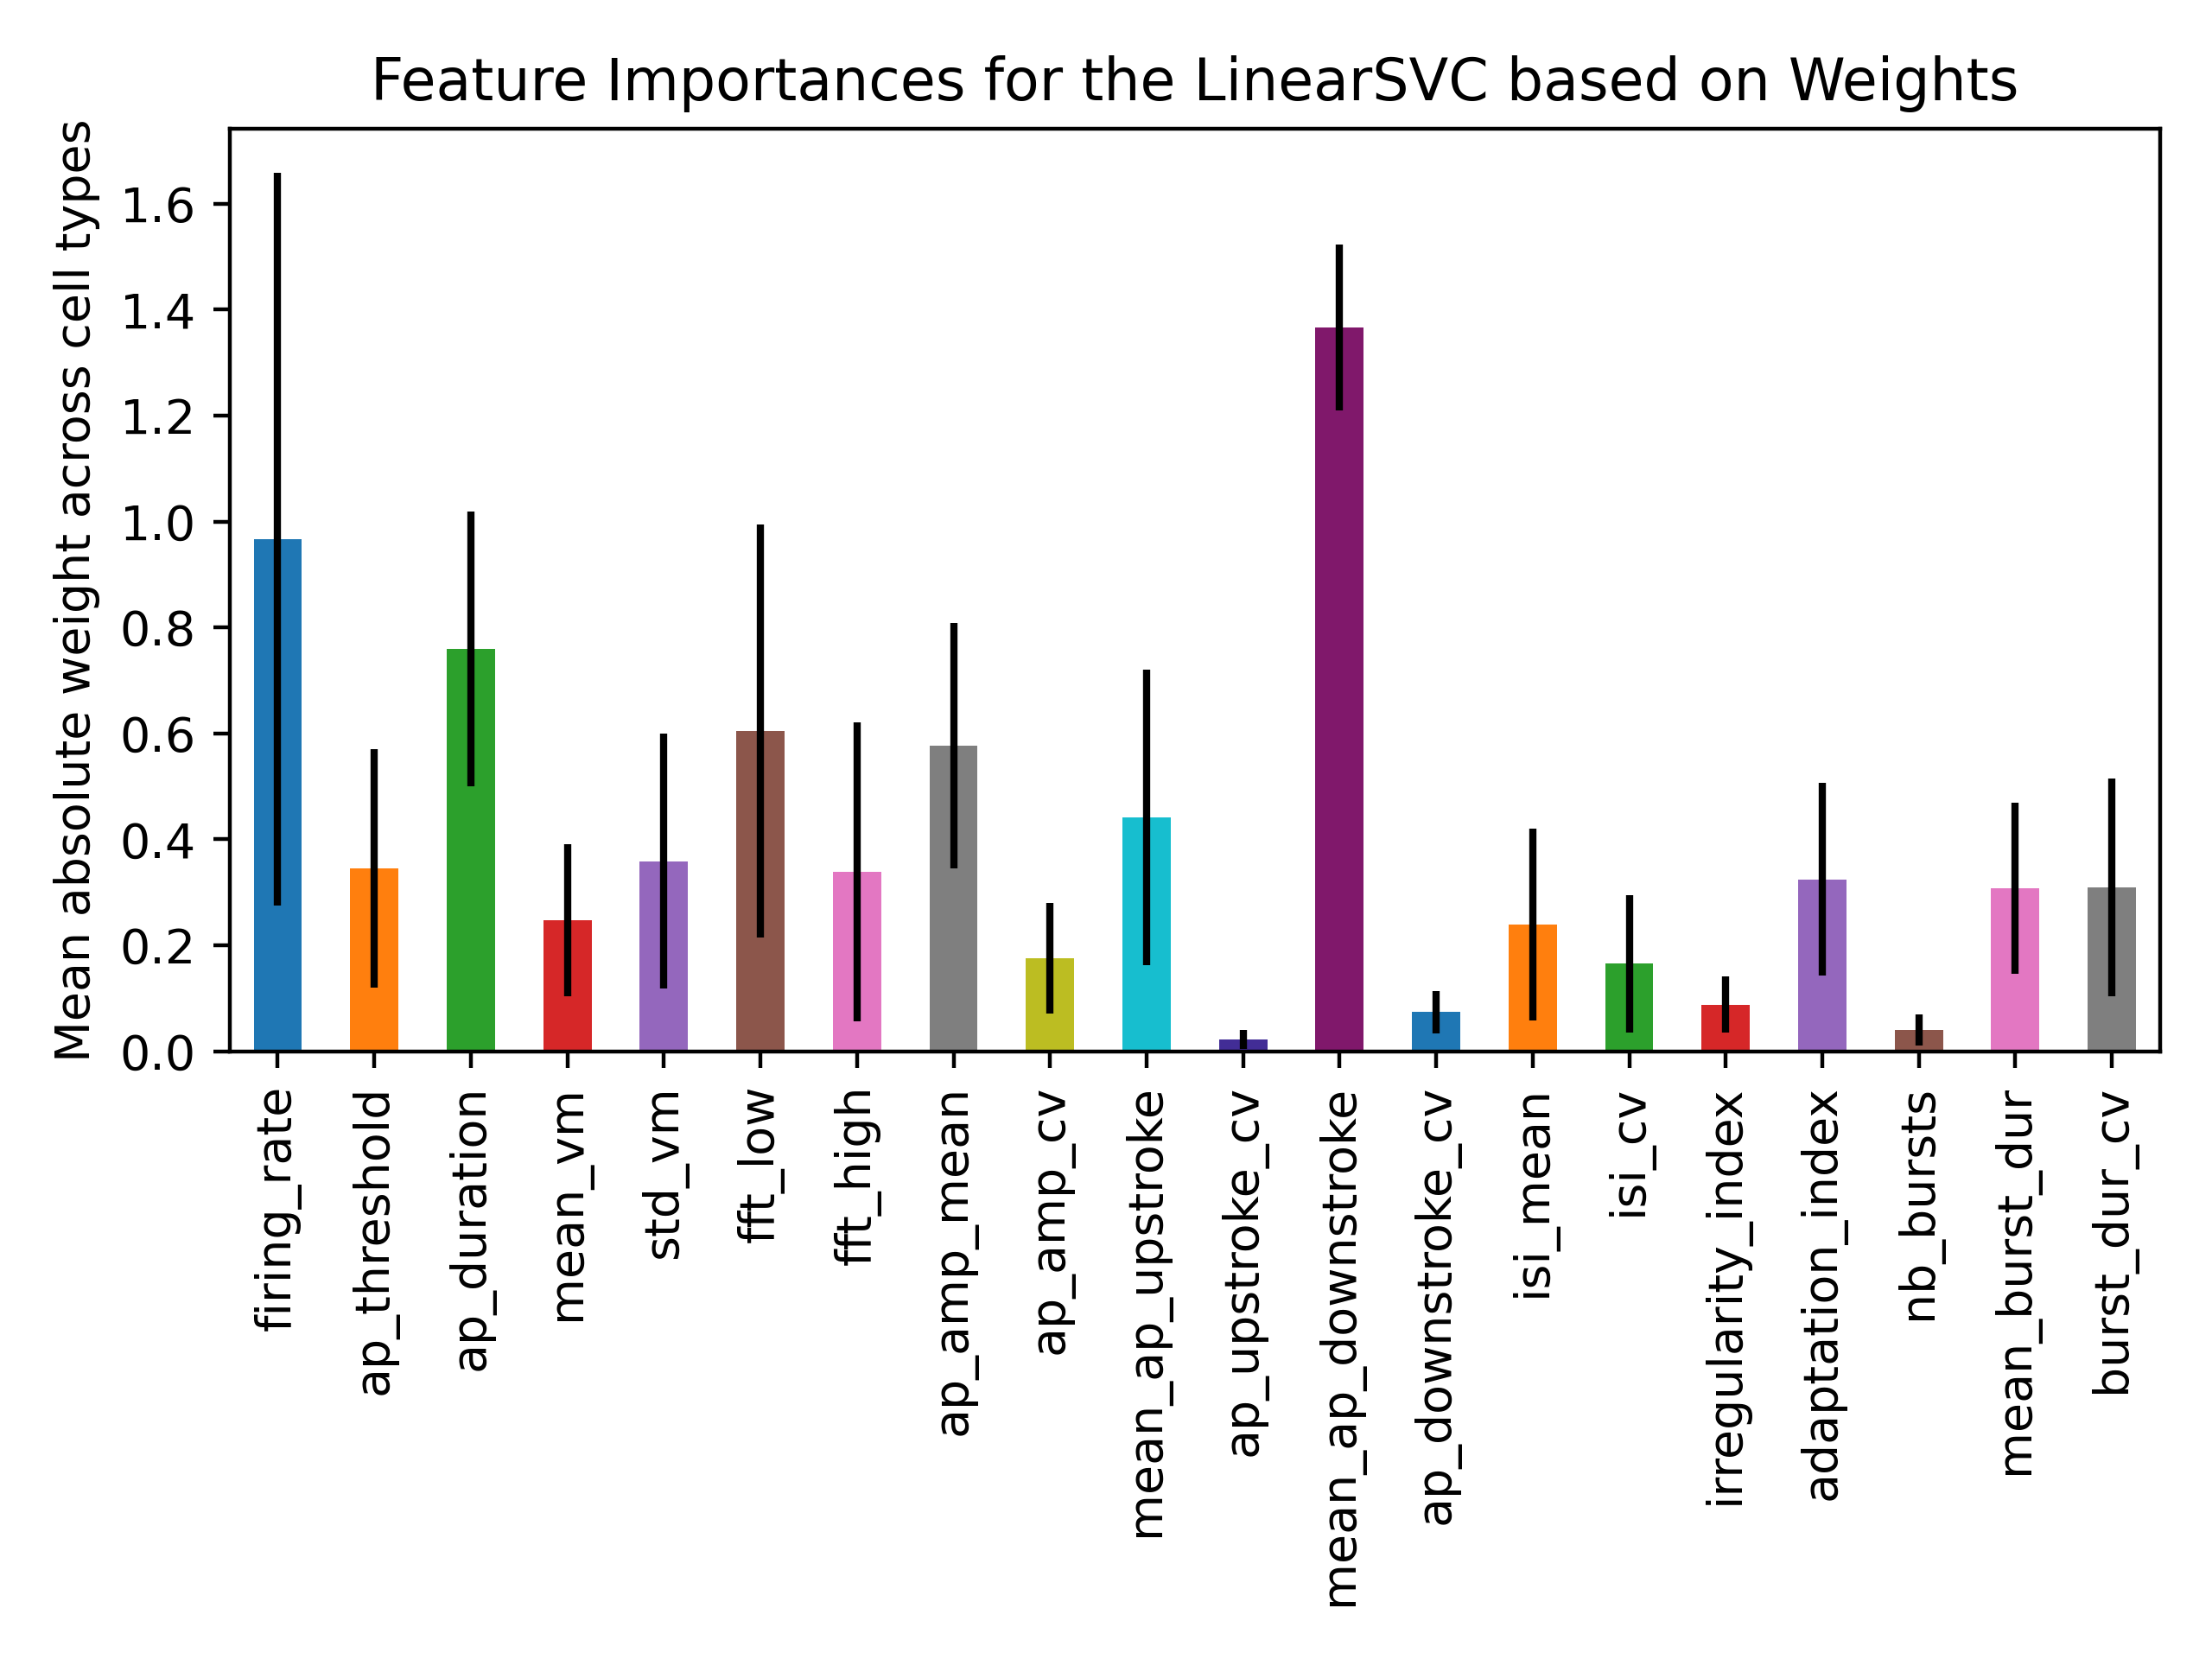
\includegraphics[width=0.9\columnwidth]{figures/feature_importance_linearsvc.png}
  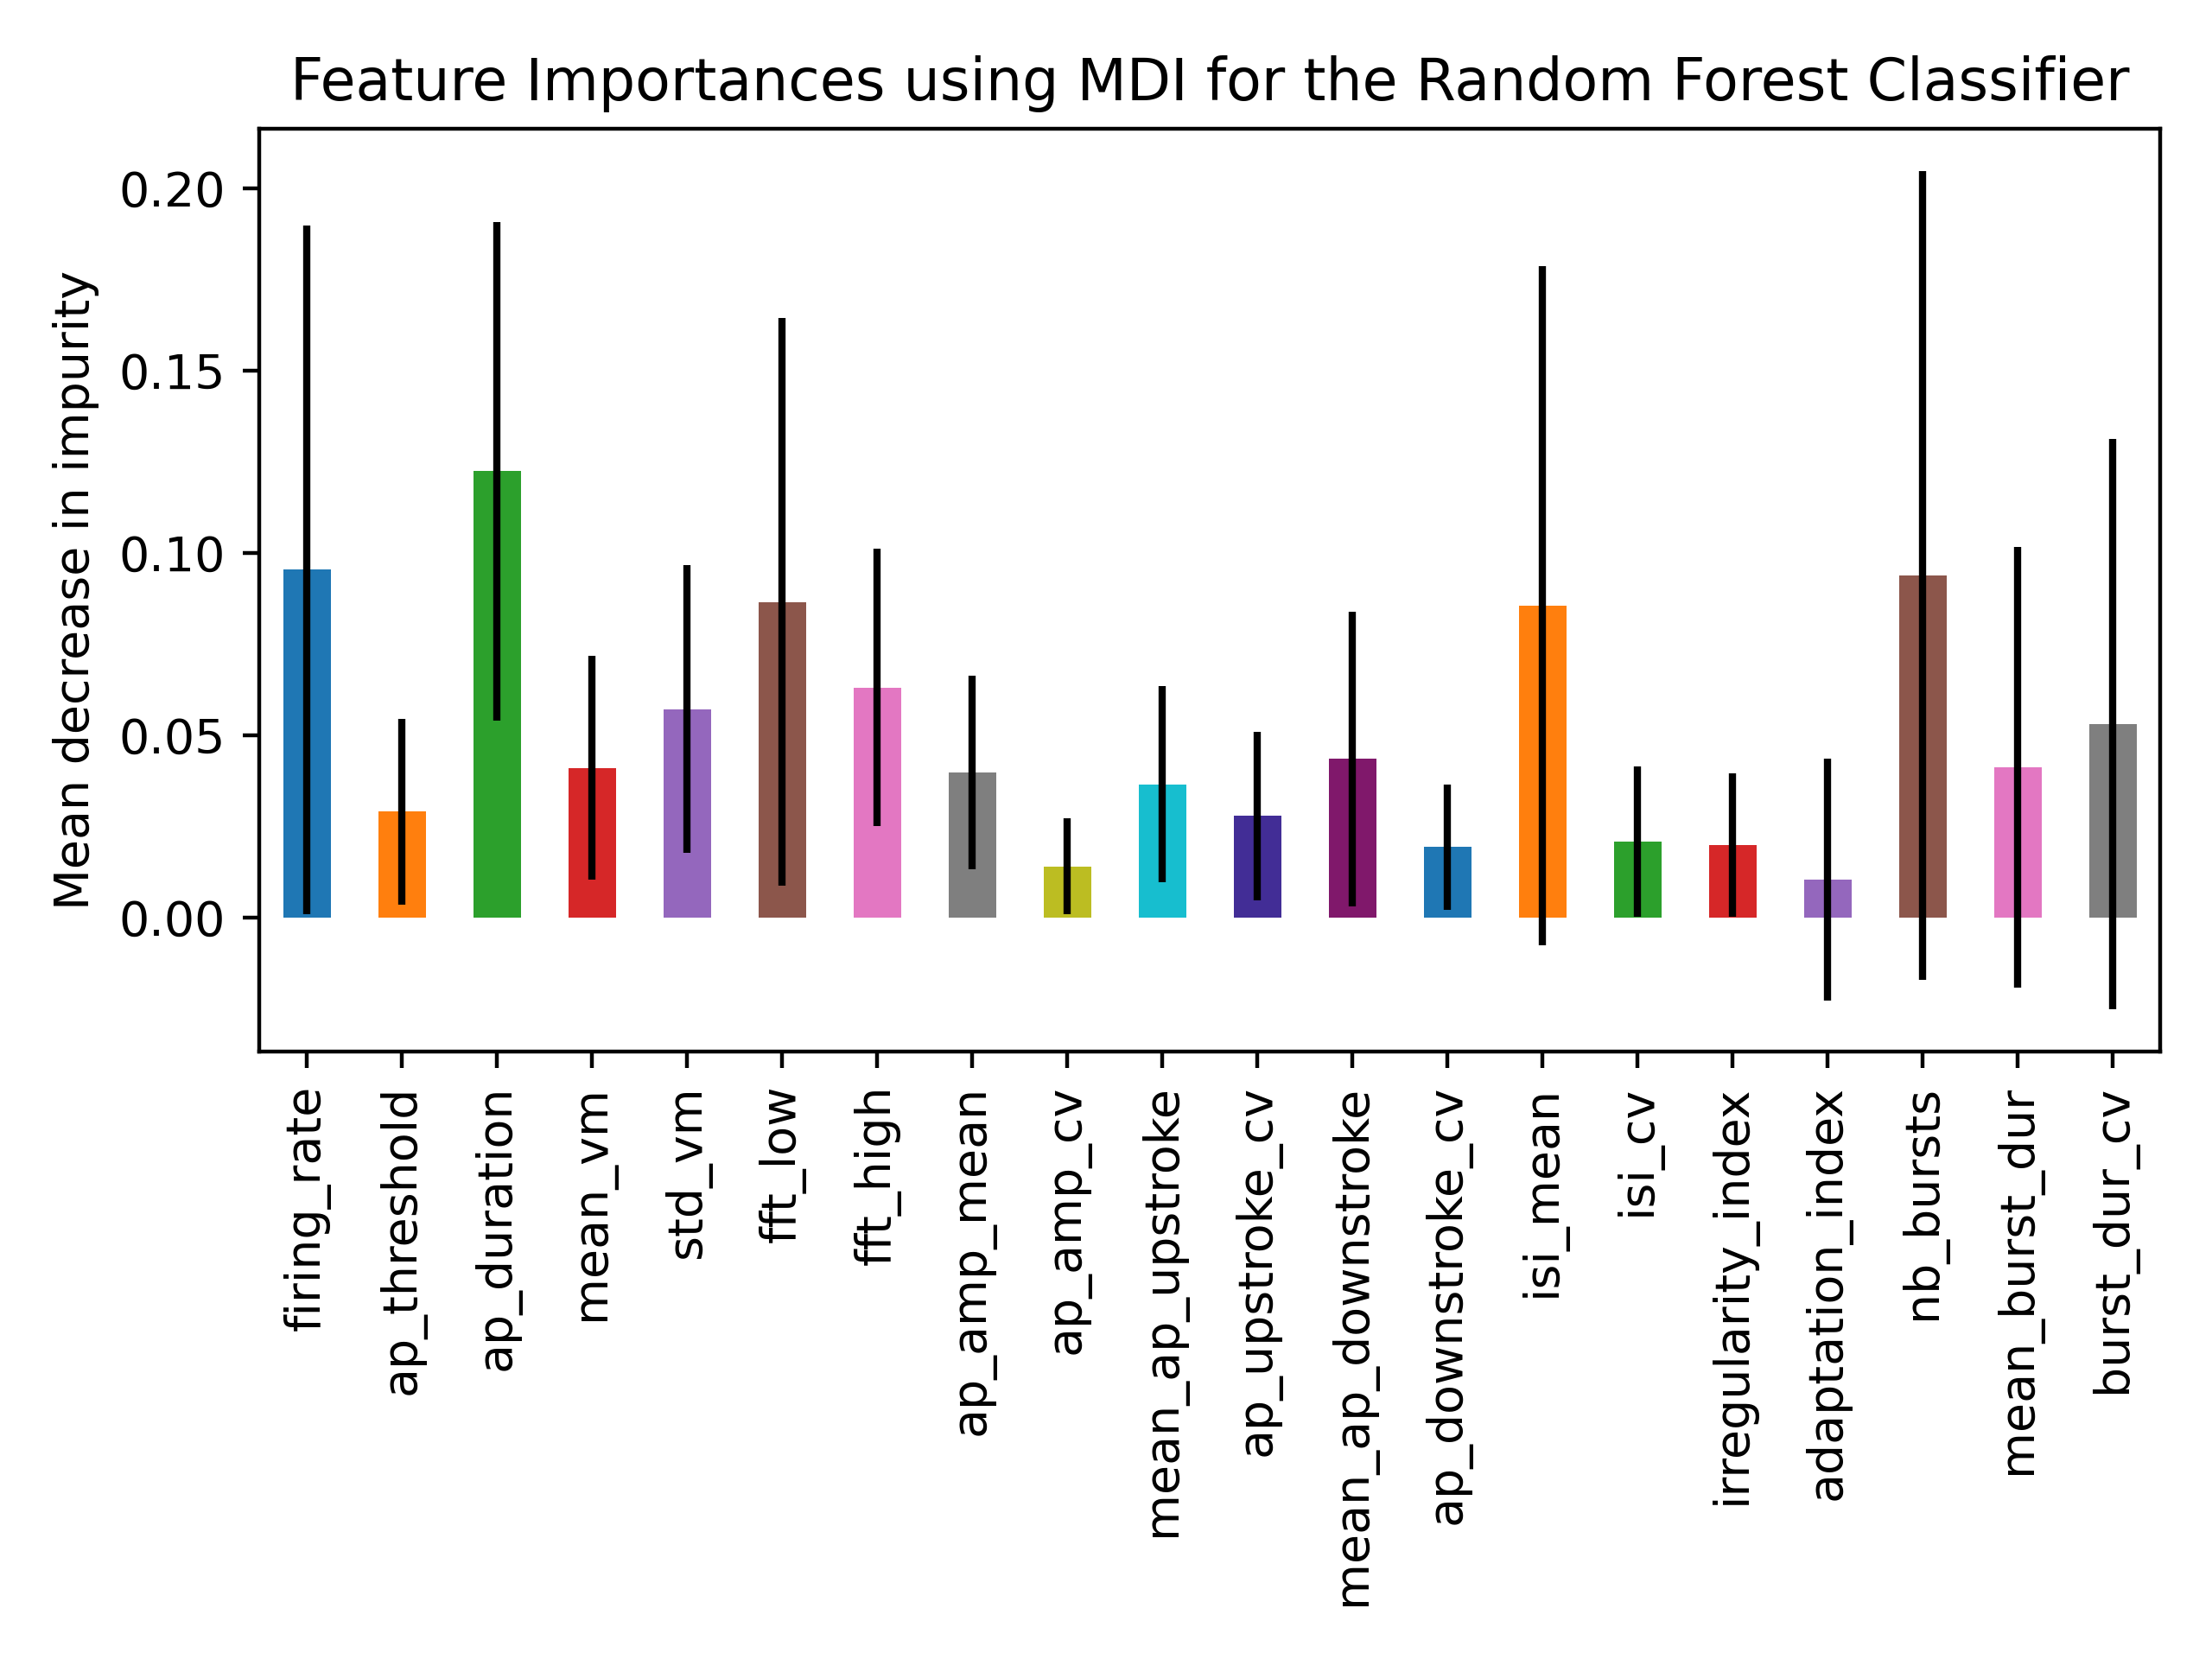
\includegraphics[width=0.9\columnwidth]{figures/feature_importance_randomforest.png}
  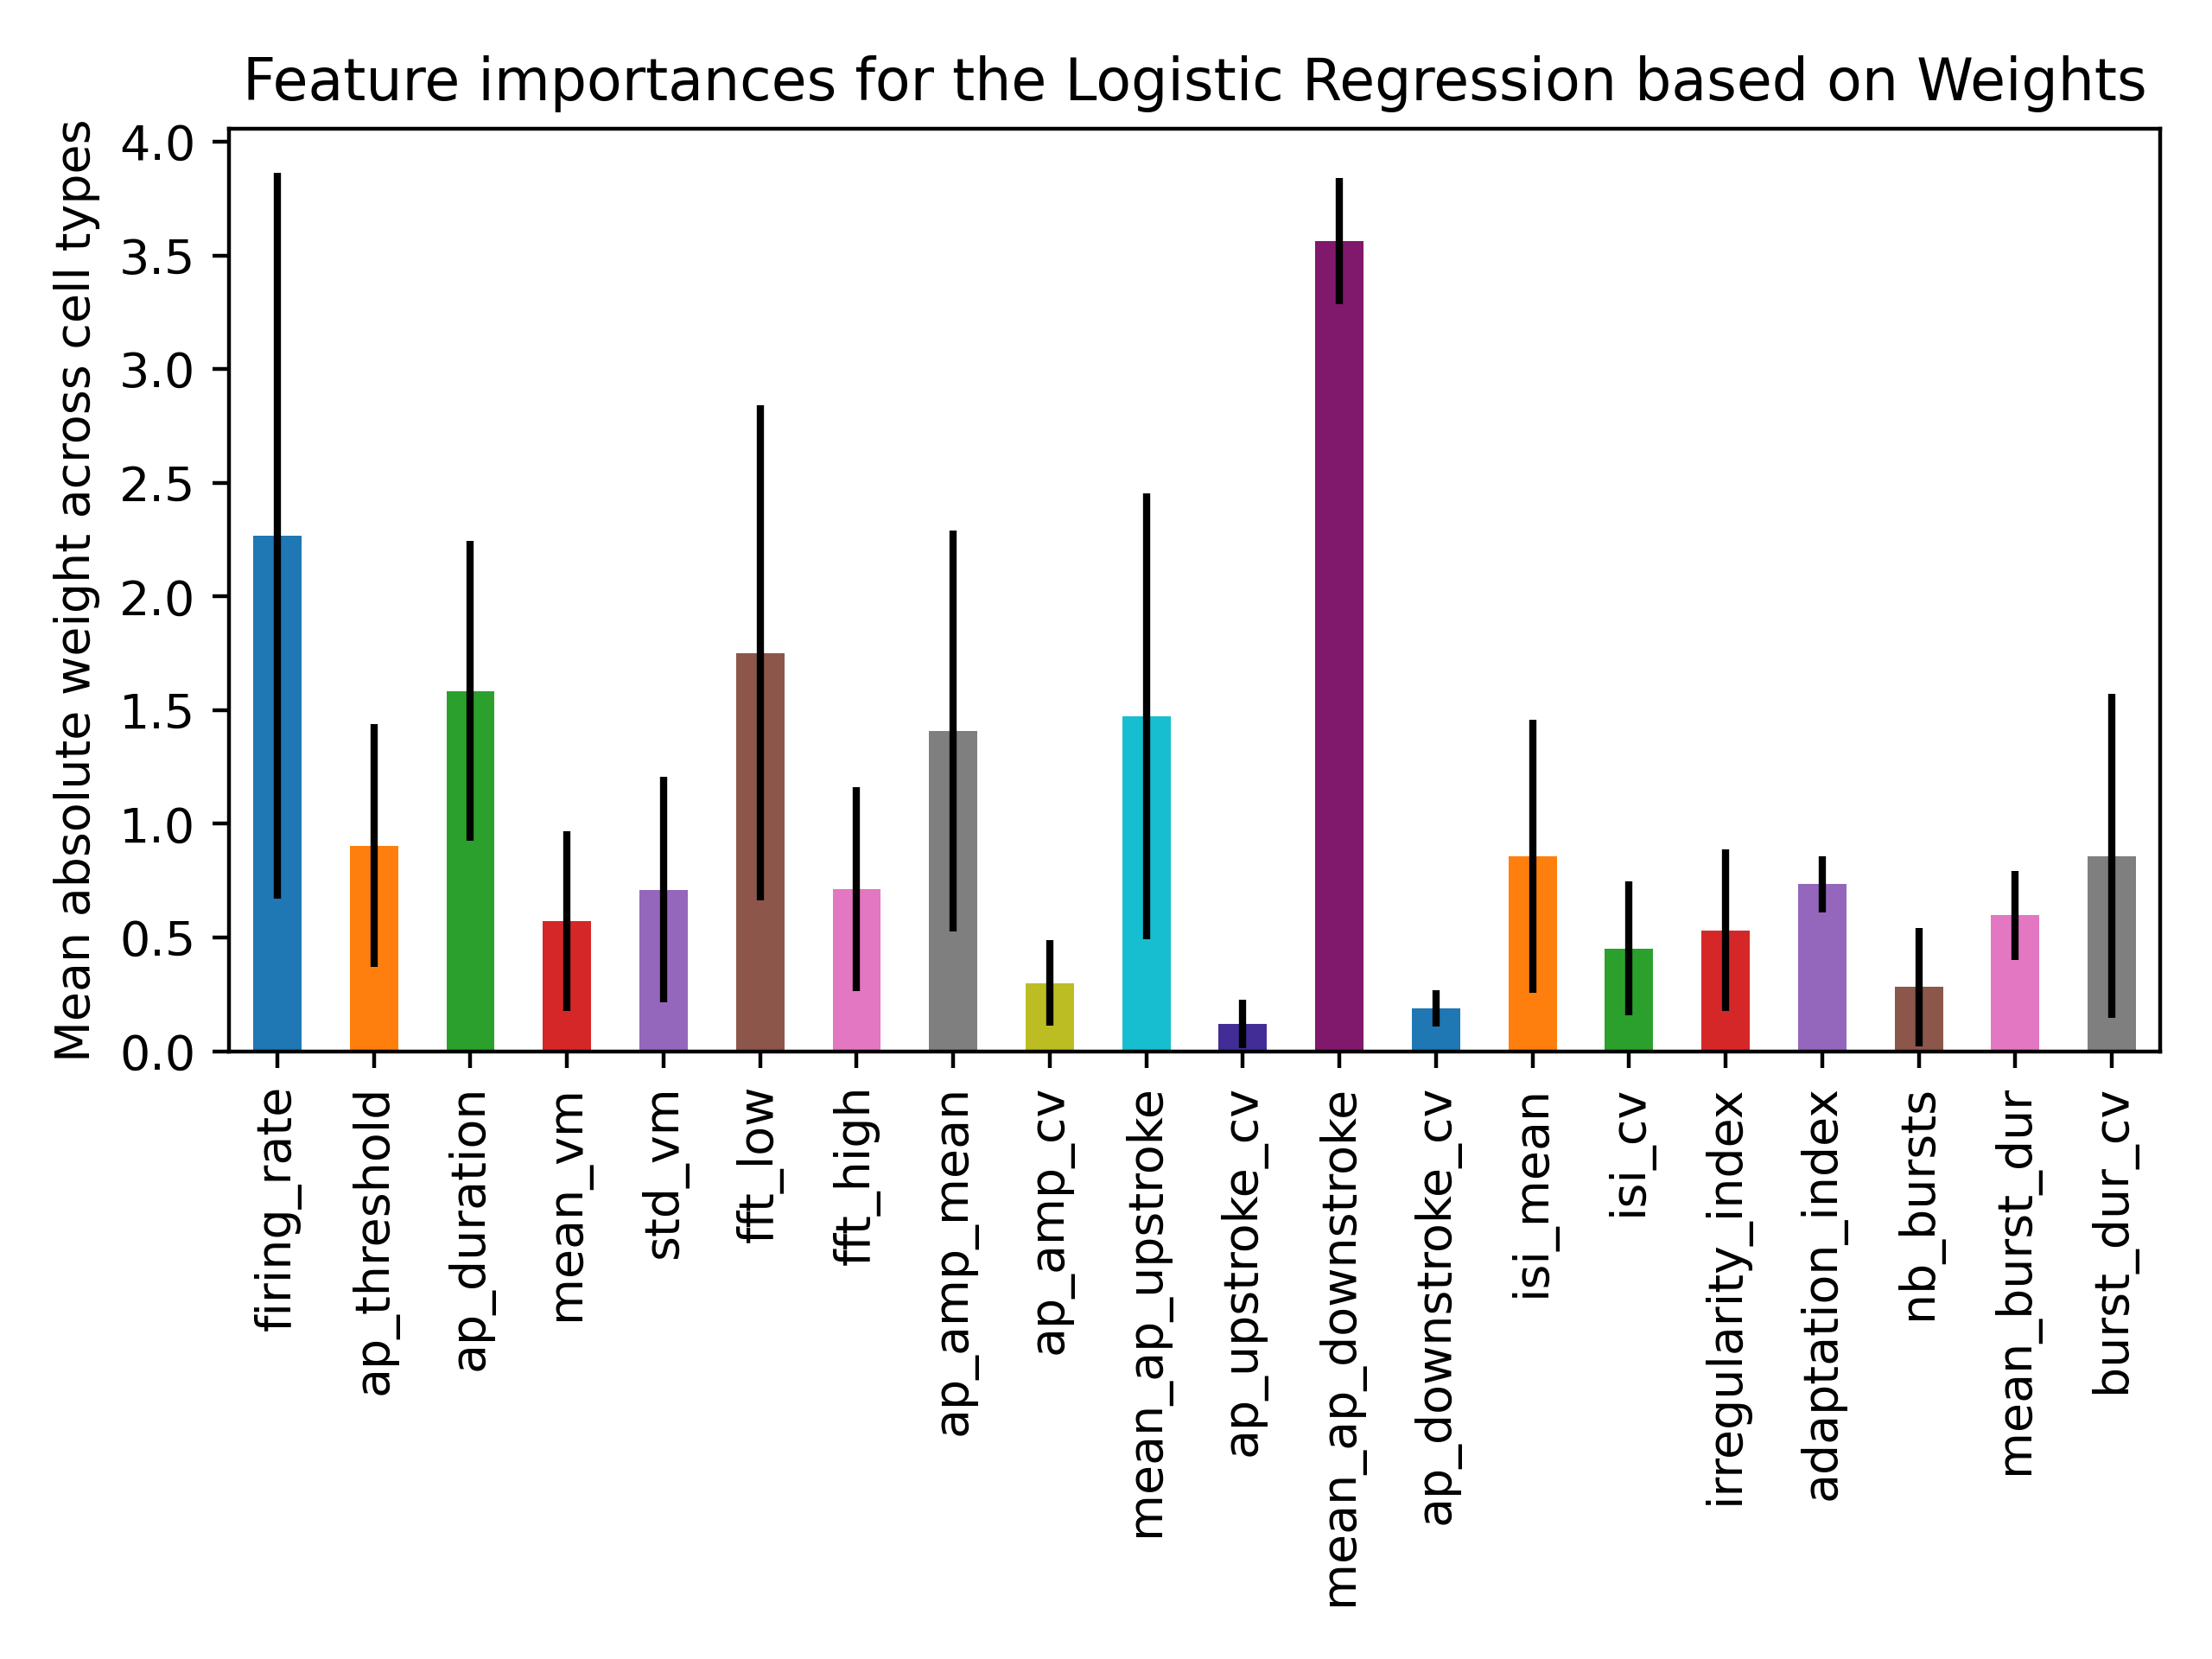
\includegraphics[width=0.9\columnwidth]{figures/feature_importance_lr.png}
  \caption{Feature importance for the top 4 best classifiers.}%
  \label{fig:feature_importances}
\end{figure*}

\subsection{Dimensionality Reduction}

\begin{figure}[h!]
  \centering
  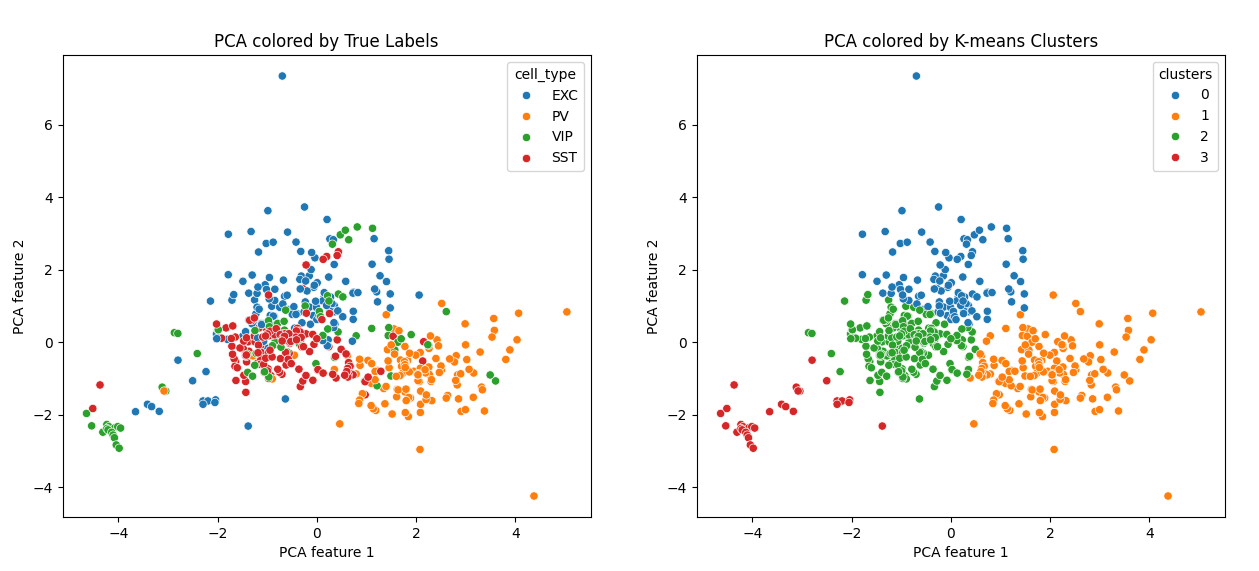
\includegraphics[width=1\columnwidth]{figures/Compare PCA 2D.png}
  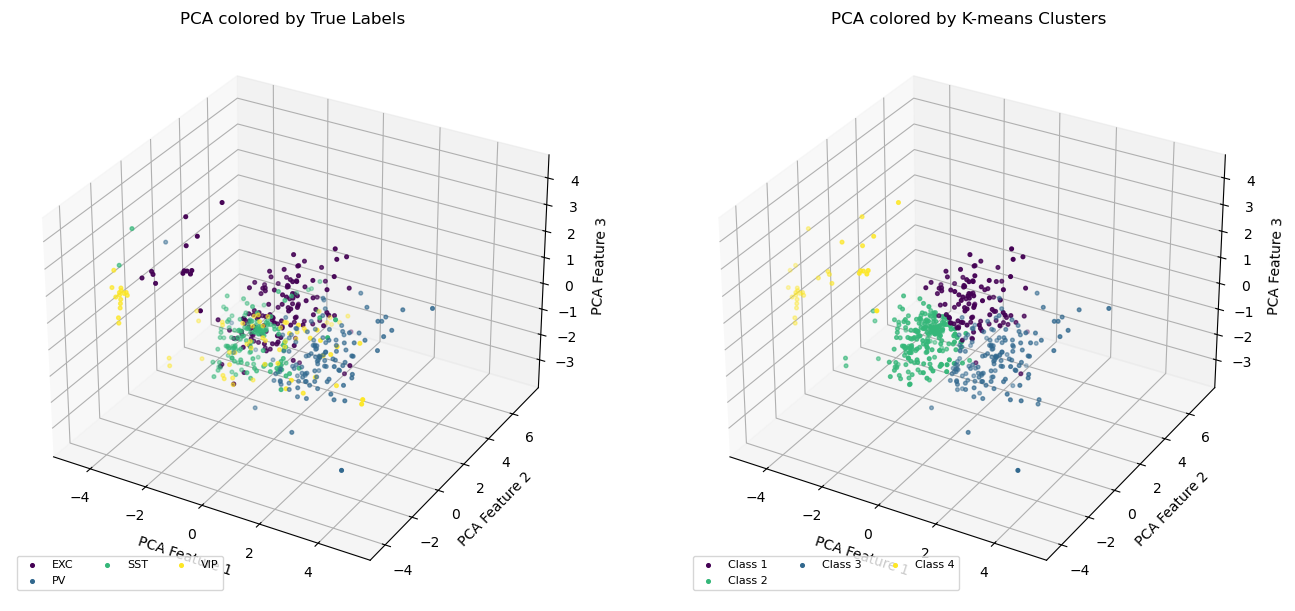
\includegraphics[width=1\columnwidth]{figures/Compare PCA 3D.png}
  \caption{2D (top row) and 3D (bottom row) PCA projections of the data. Left column is colored by true labels, and right column is colored by K-Means clustering.}%
  \label{fig:pca}
\end{figure}

\begin{figure}[h!]
  \centering
  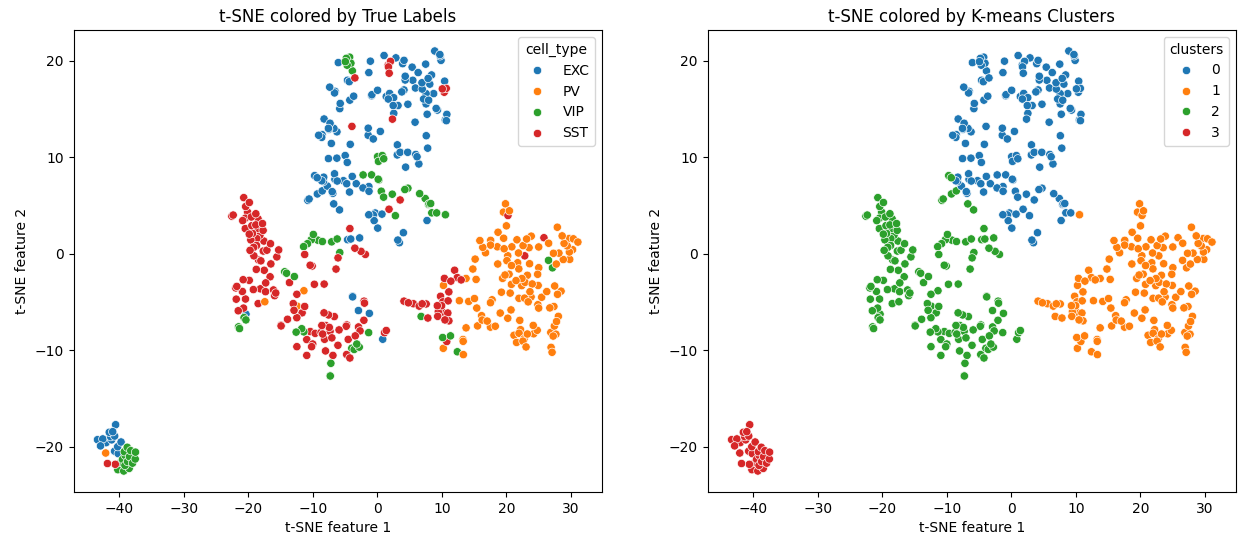
\includegraphics[width=1\columnwidth]{figures/Compare t-SNE 2D.png}
  \includegraphics[width=1\columnwidth]{figures/Compare t-SNE 3D.png}
  \caption{2D (top row) and 3D (bottom row) t-SNE projections of the data. Left column is colored by true labels, and right column is colored by K-Means clustering.}%
  \label{fig:t-SNE}
\end{figure}

\begin{figure}[h!]
  \centering
  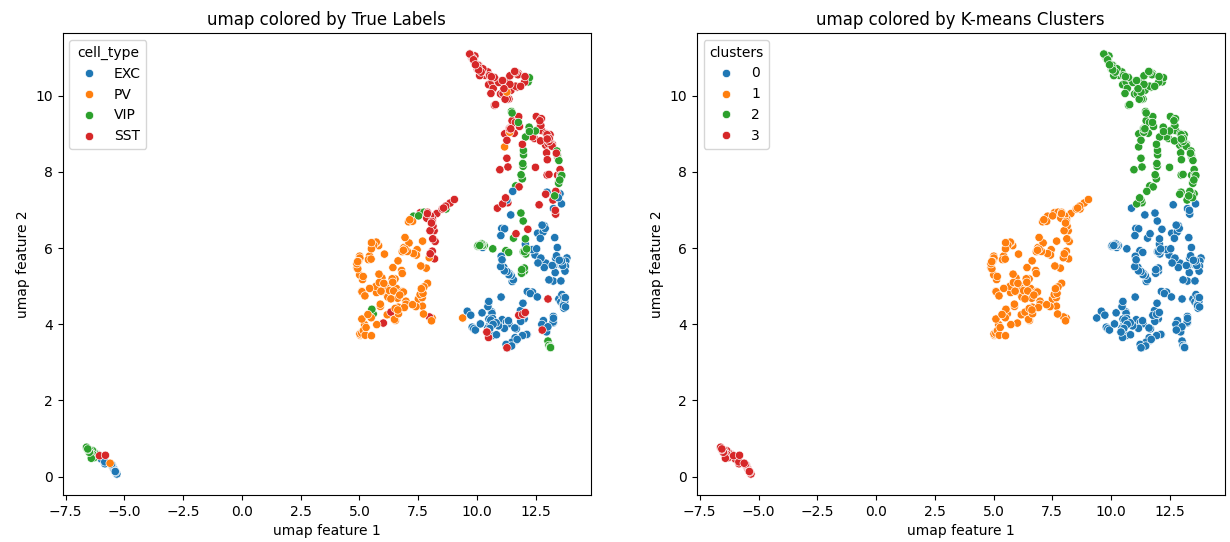
\includegraphics[width=1\columnwidth]{figures/Compare UMAP 2D.png}
  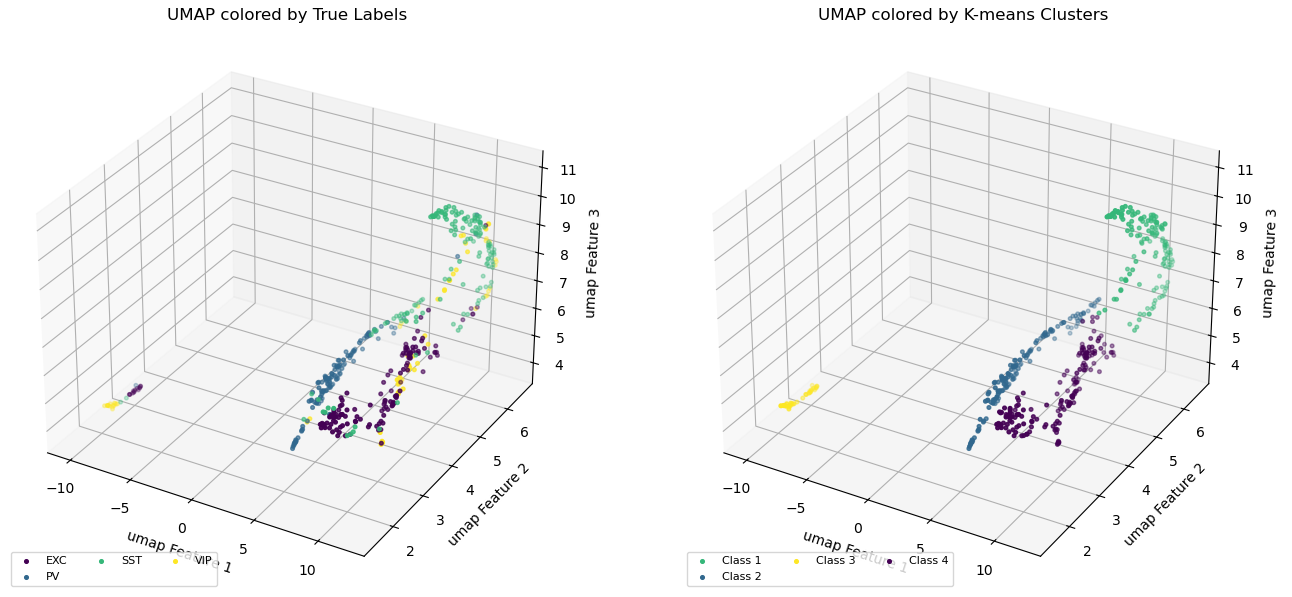
\includegraphics[width=1\columnwidth]{figures/Compare UMAP 3D.png}
  \caption{2D (top row) and 3D (bottom row) UMAP projections of the data. Left column is colored by true labels, and right column is colored by K-Means clustering.}%
  \label{fig:umap}
\end{figure}

From both PCA, t-SNE and UMAP (Fig. \ref{fig:pca}, \ref{fig:t-SNE}, \ref{fig:umap}), there emerges similar patterns in the way cell classes are predisposed. PV cells seem to be more separated, and less mixed with other cell types. VIP cells are scattered and are not captured within a region of space, unlike the other cell classes.
SST and EXC cells are depicted close to each other.
A small, mixed class grouping of points is always in the bottom left corner of 2D projections. 

\subsection{Unsupervised Performance}

\begin{figure}[h!]
  \centering
  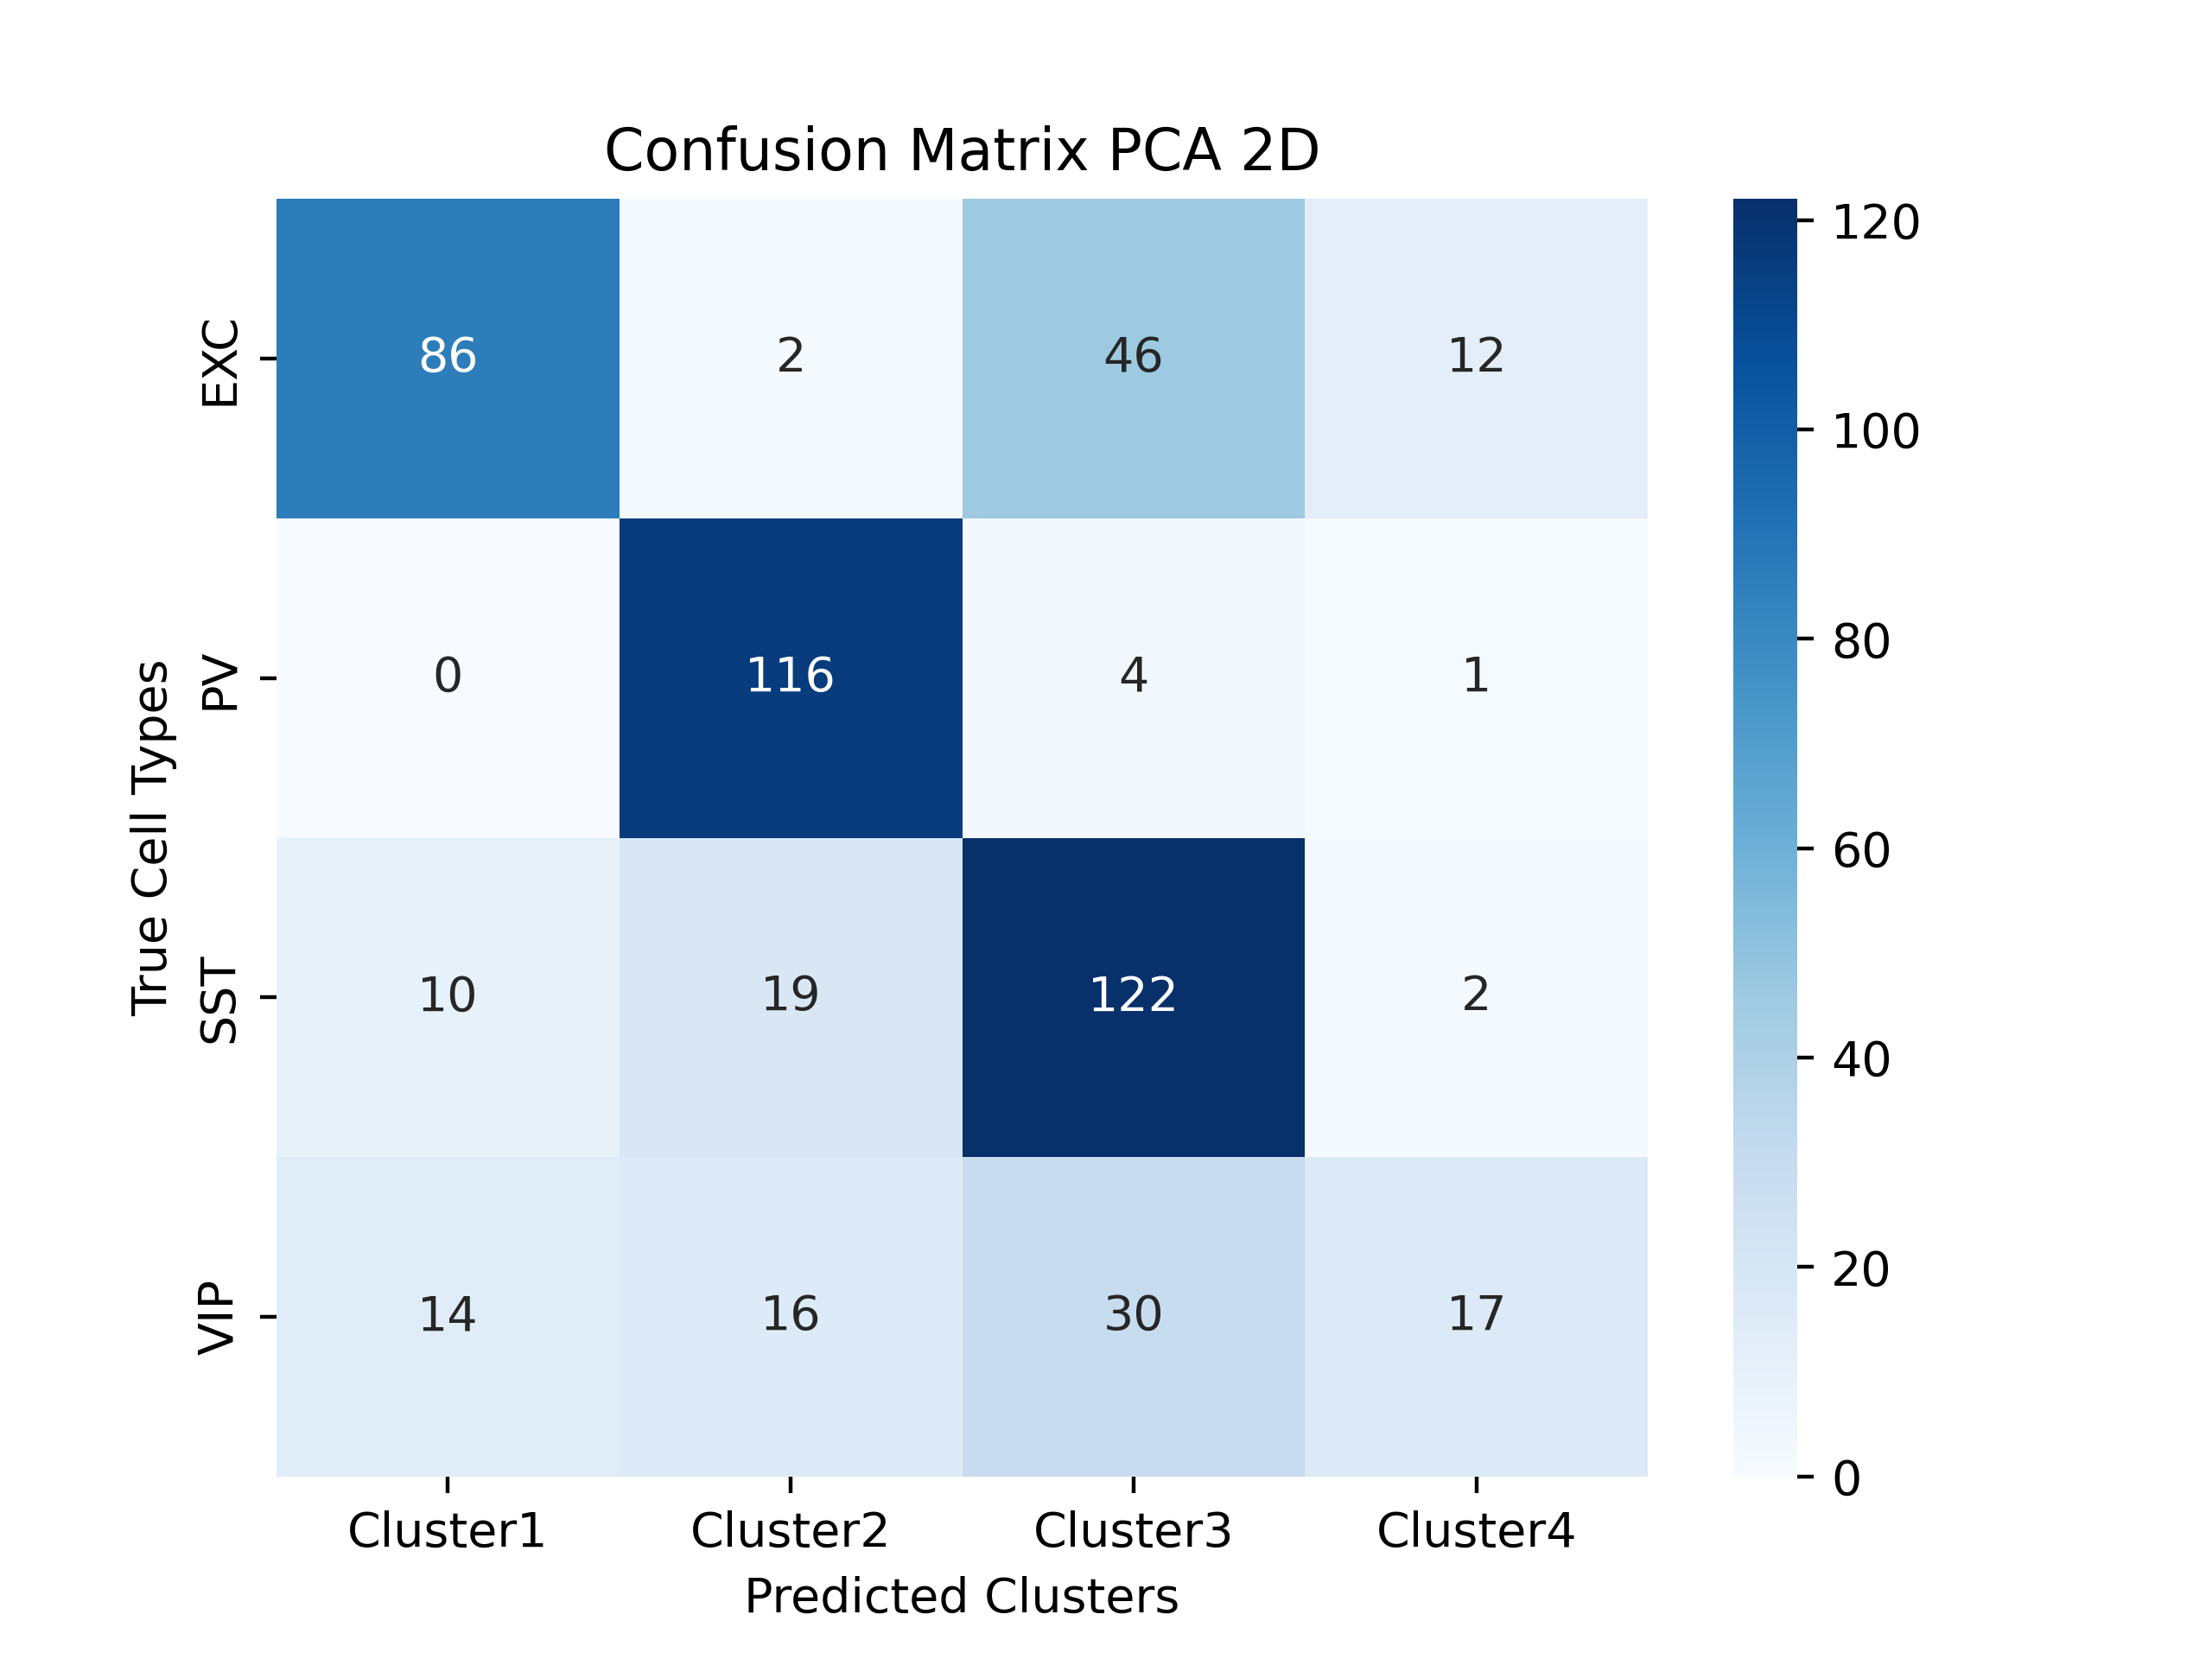
\includegraphics[width=0.45\columnwidth]{figures/Confusion Matrix PCA 2D.png}
  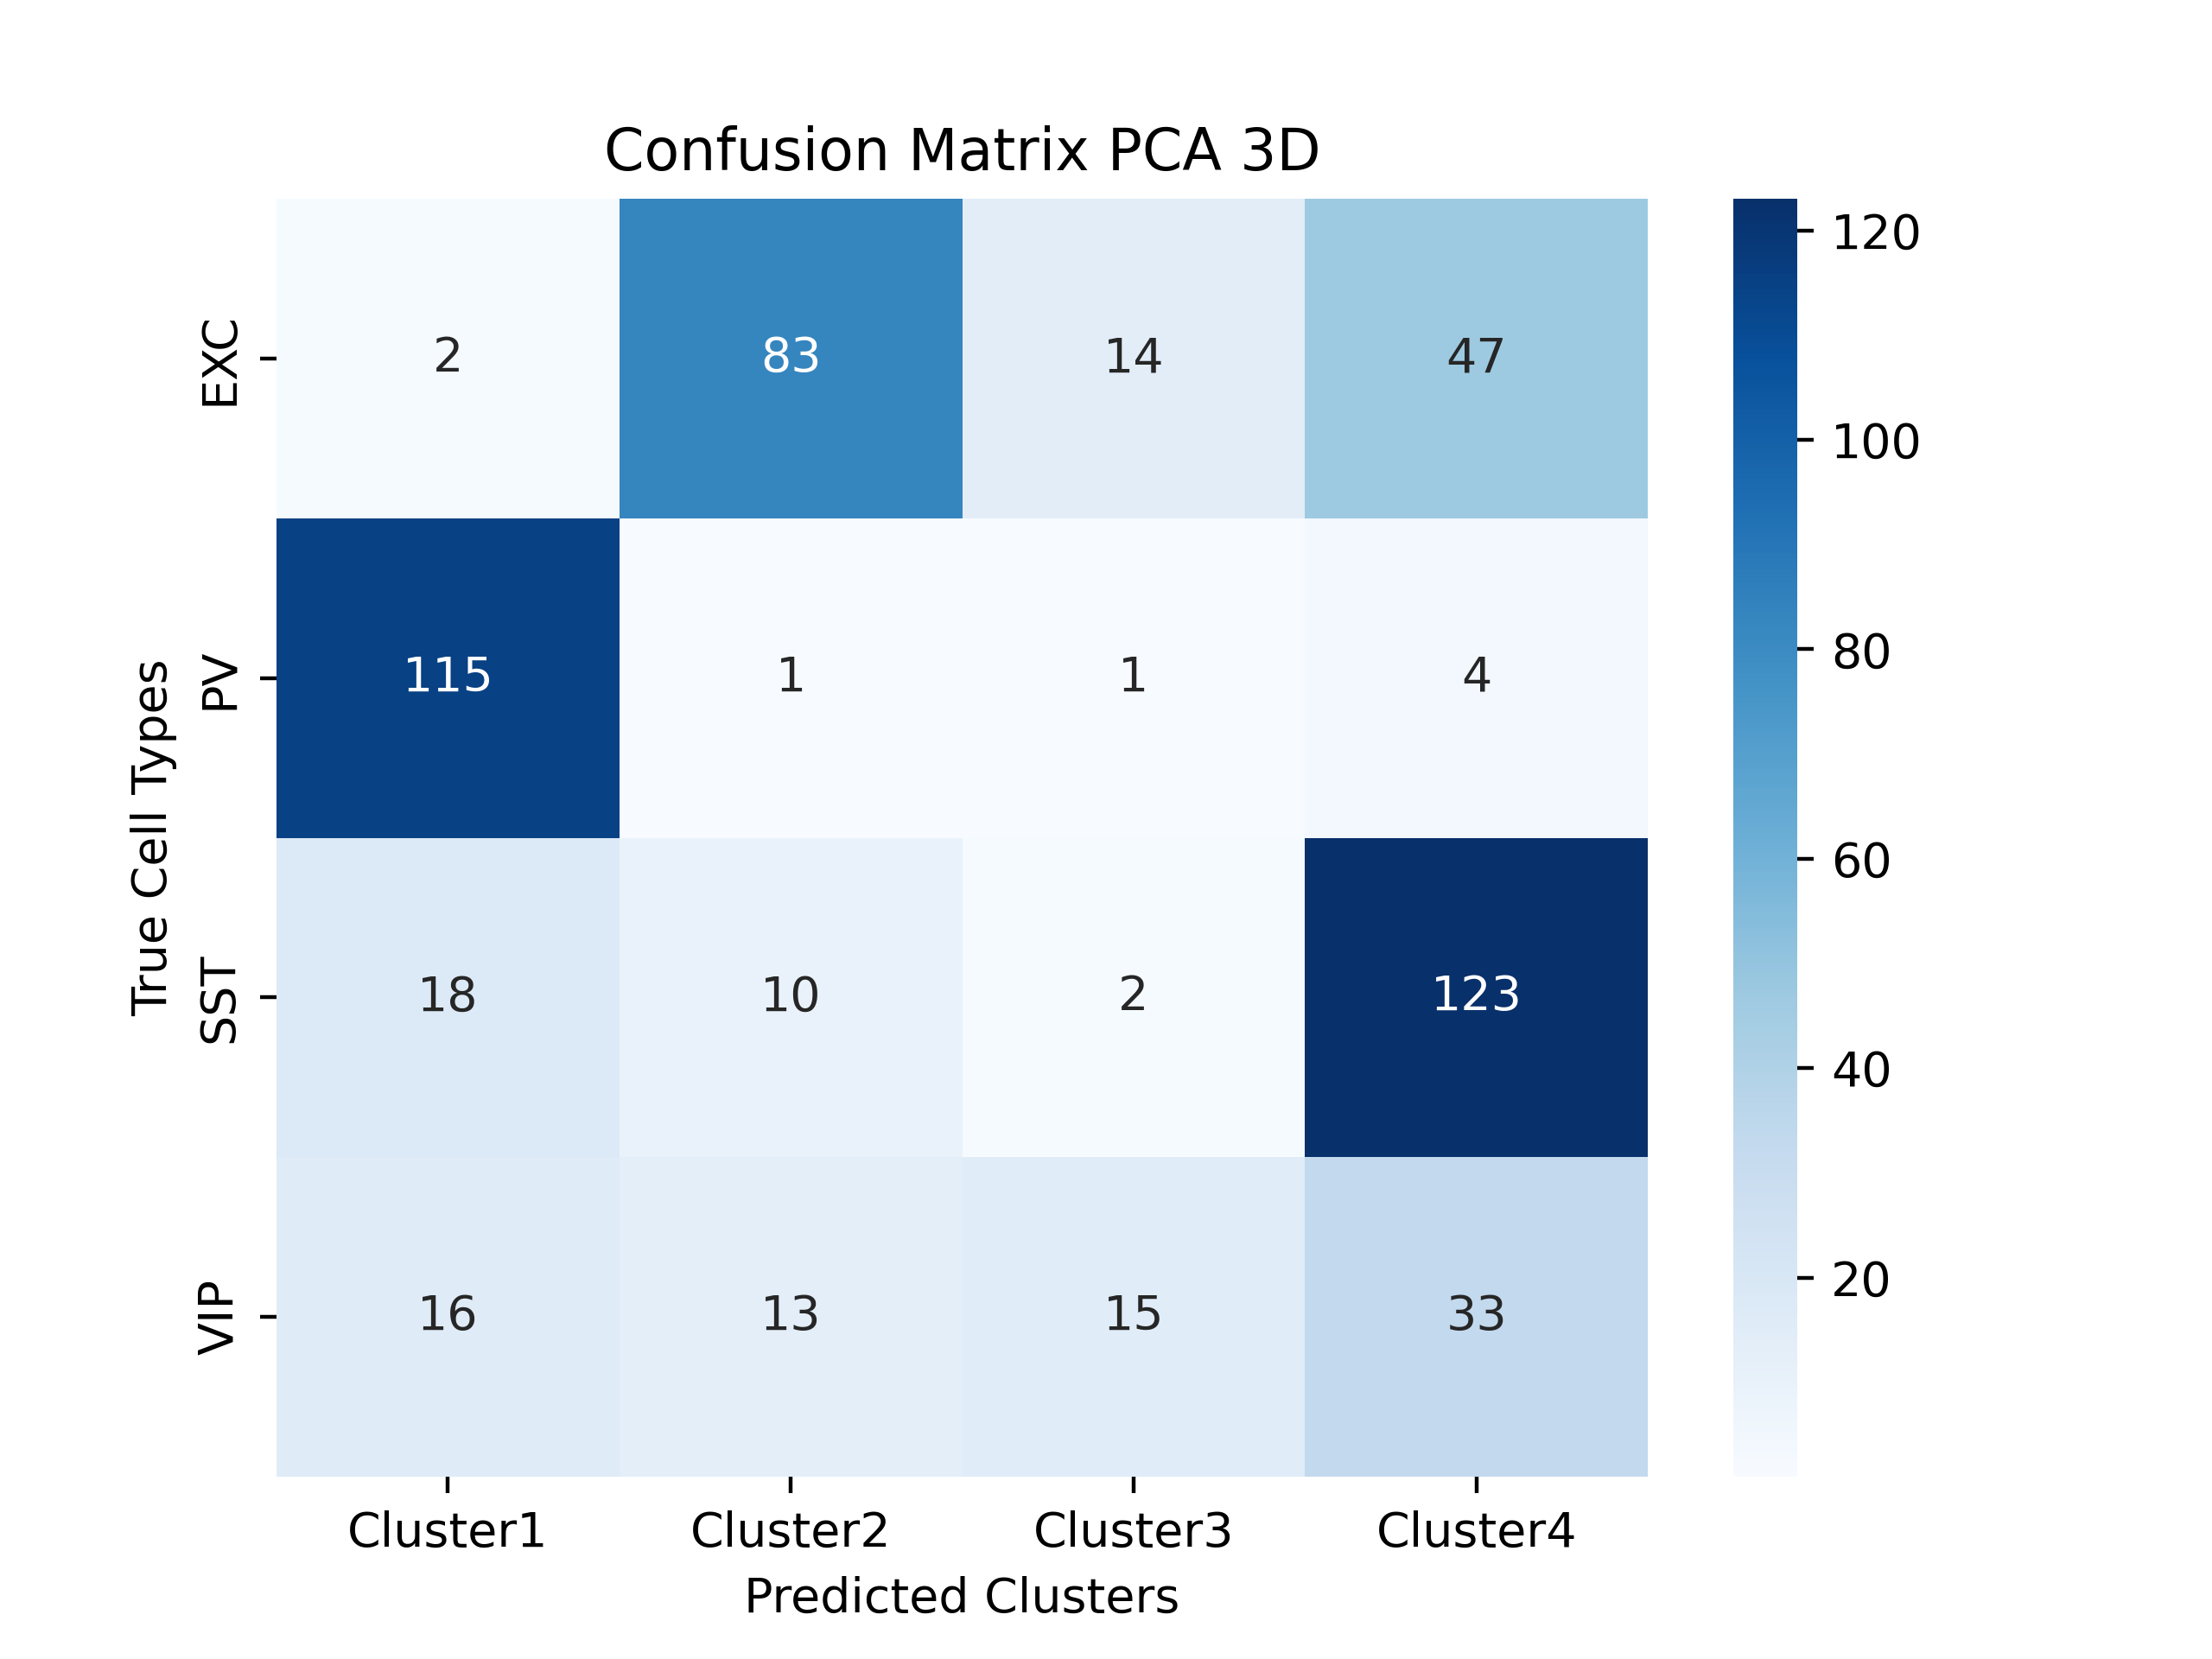
\includegraphics[width=0.45\columnwidth]{figures/Confusion Matrix PCA 3D.png}
  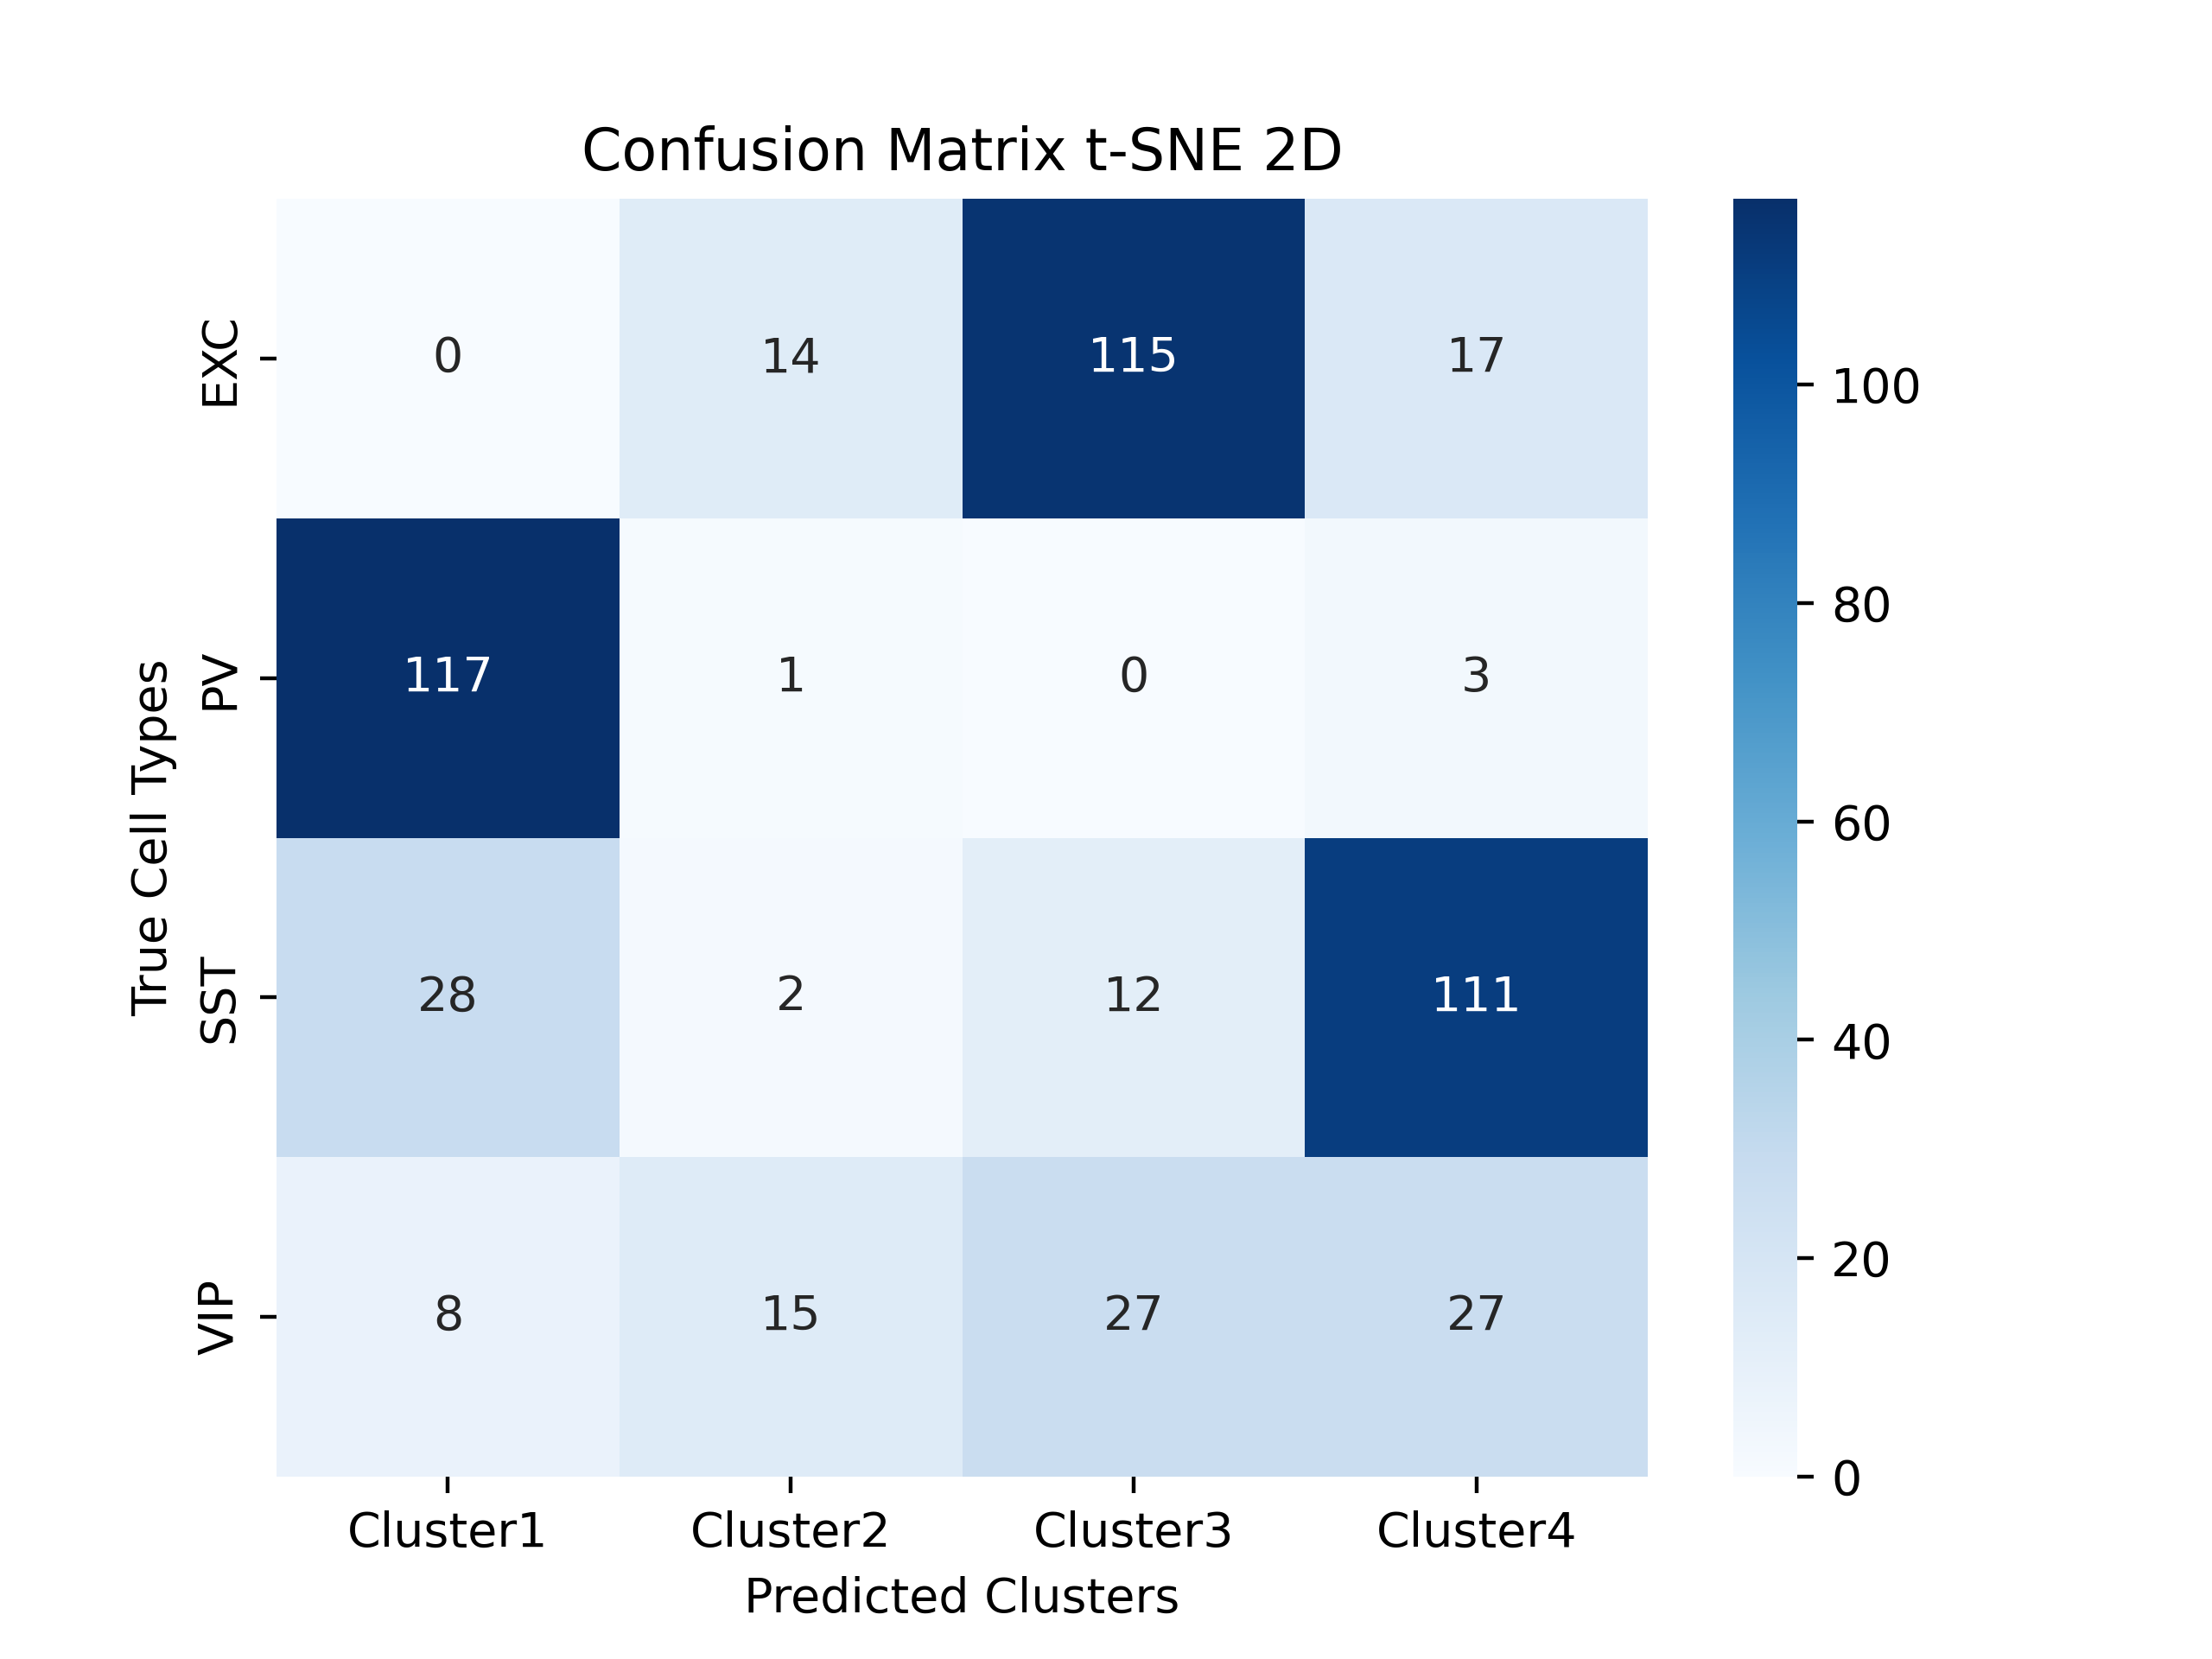
\includegraphics[width=0.45\columnwidth]{figures/Confusion Matrix t-SNE 2D.png}
  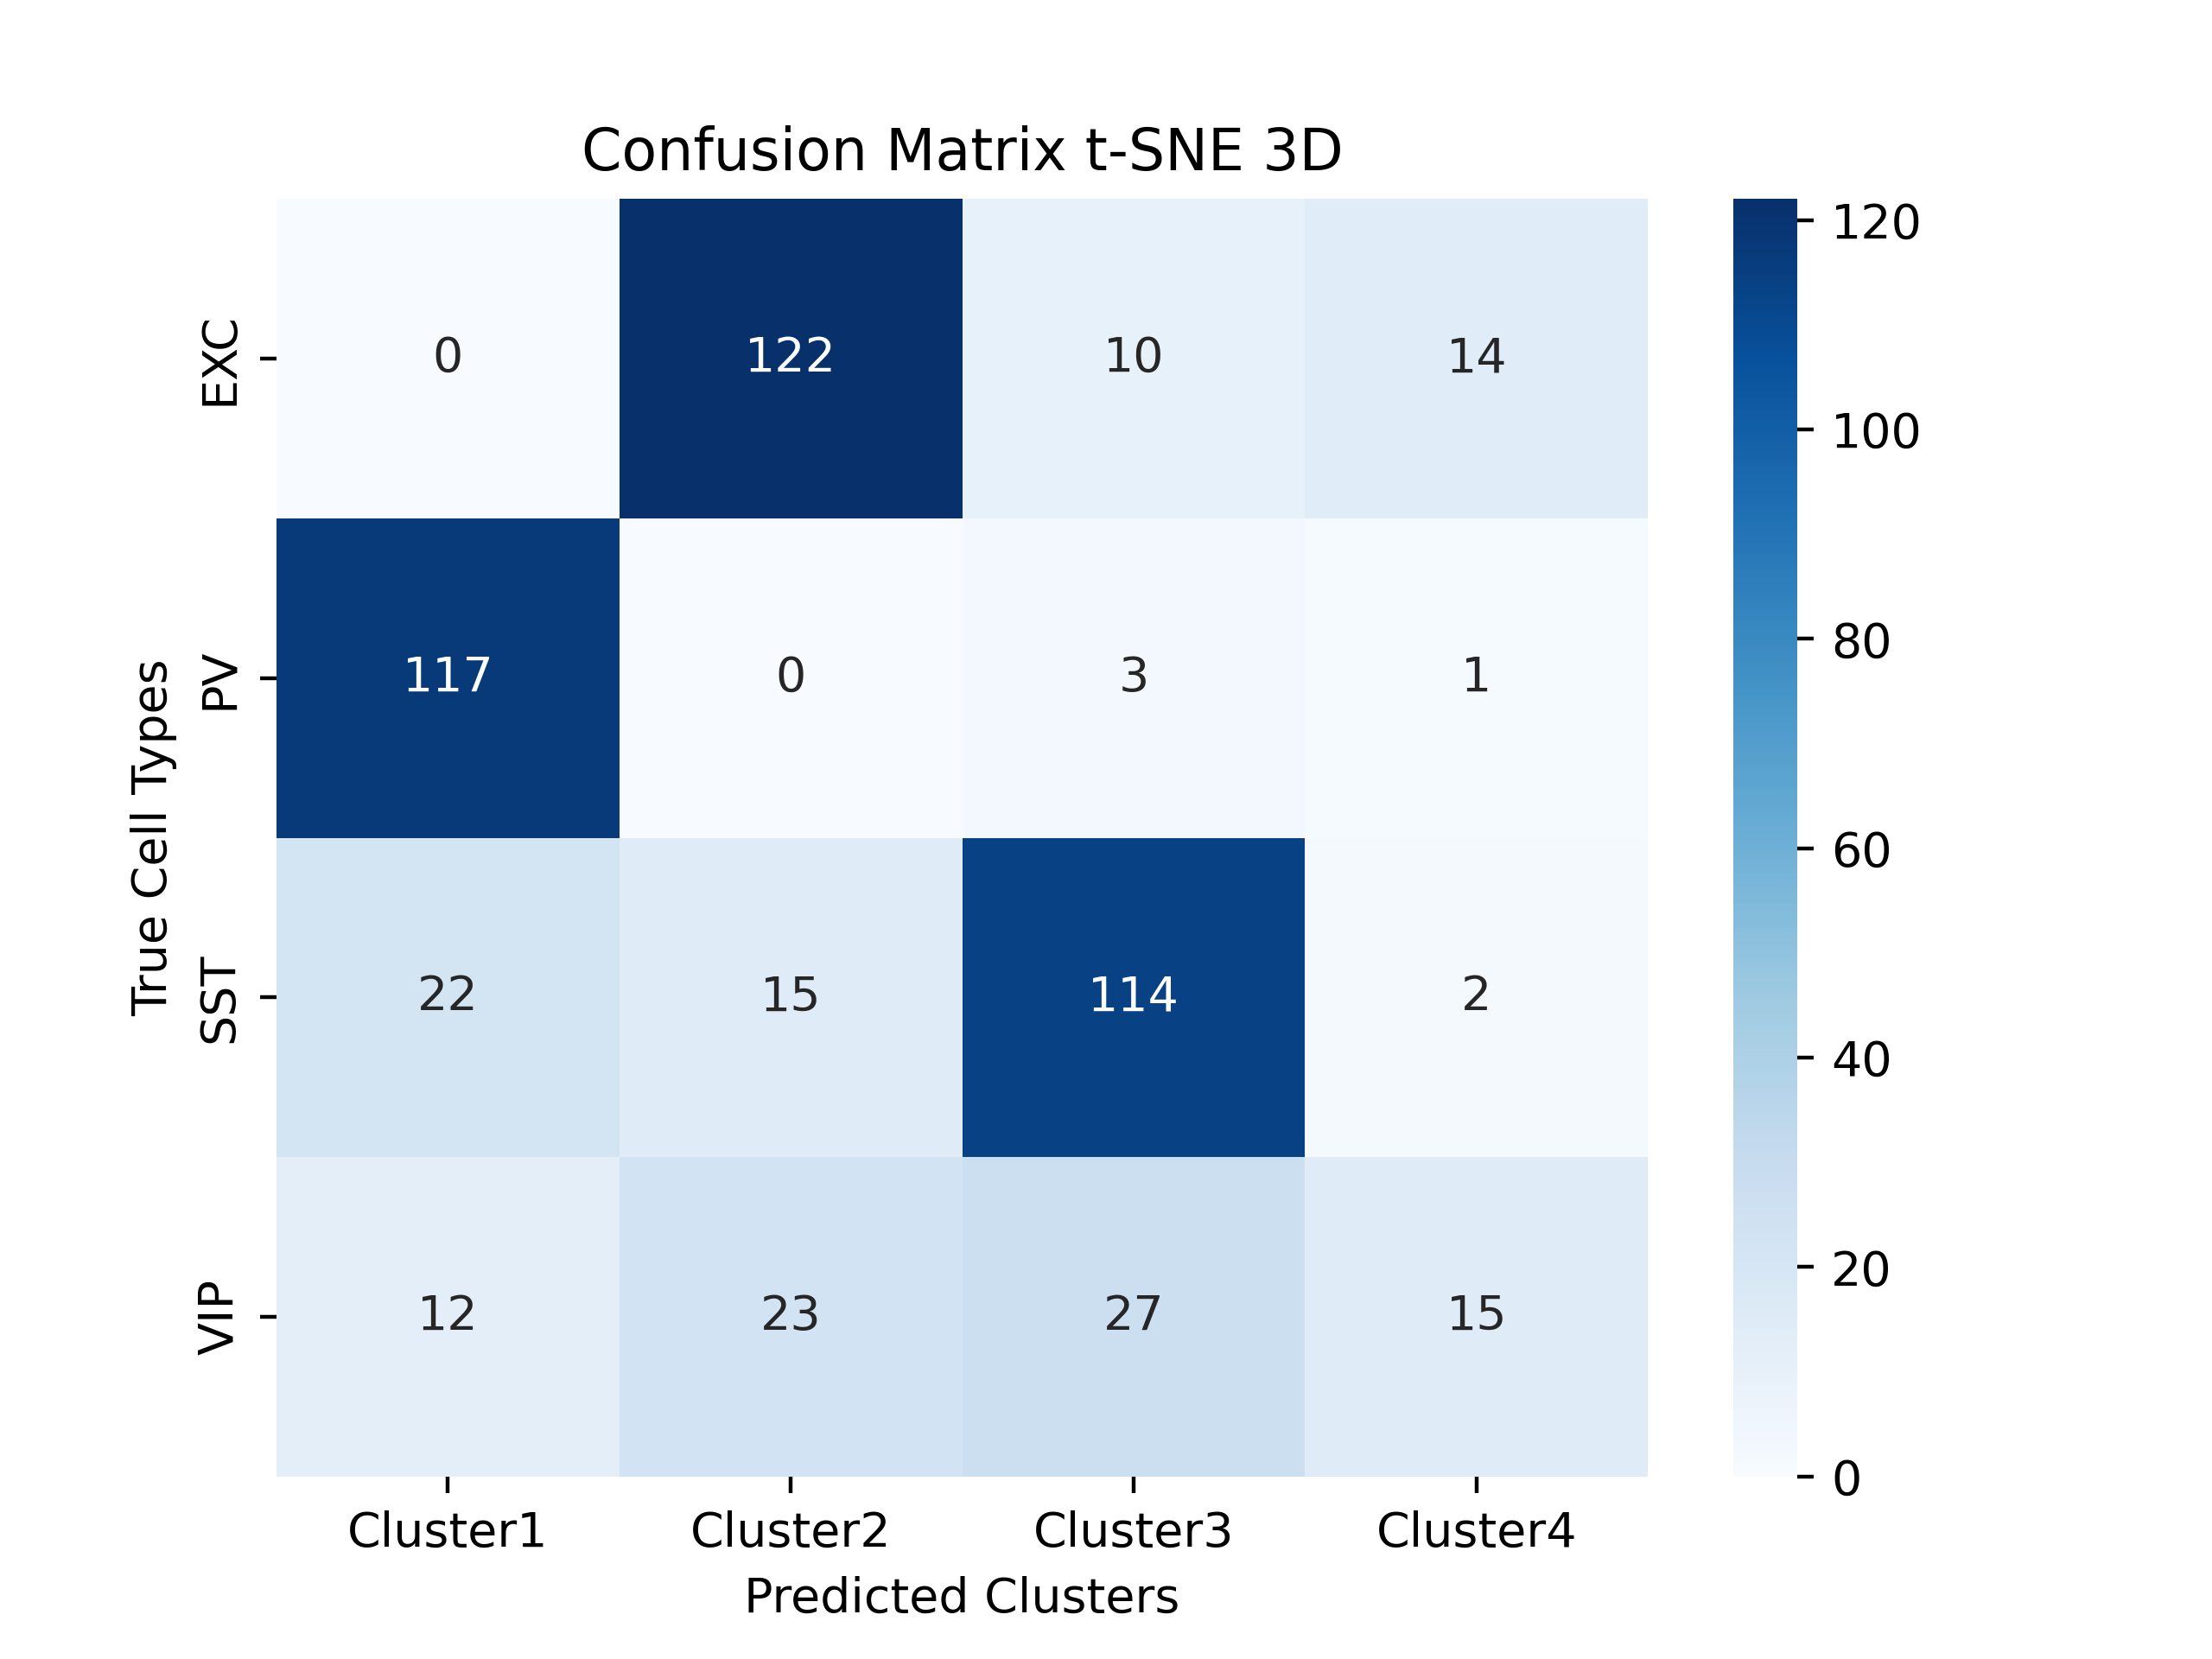
\includegraphics[width=0.45\columnwidth]{figures/Confusion Matrix t-SNE 3D.png}
  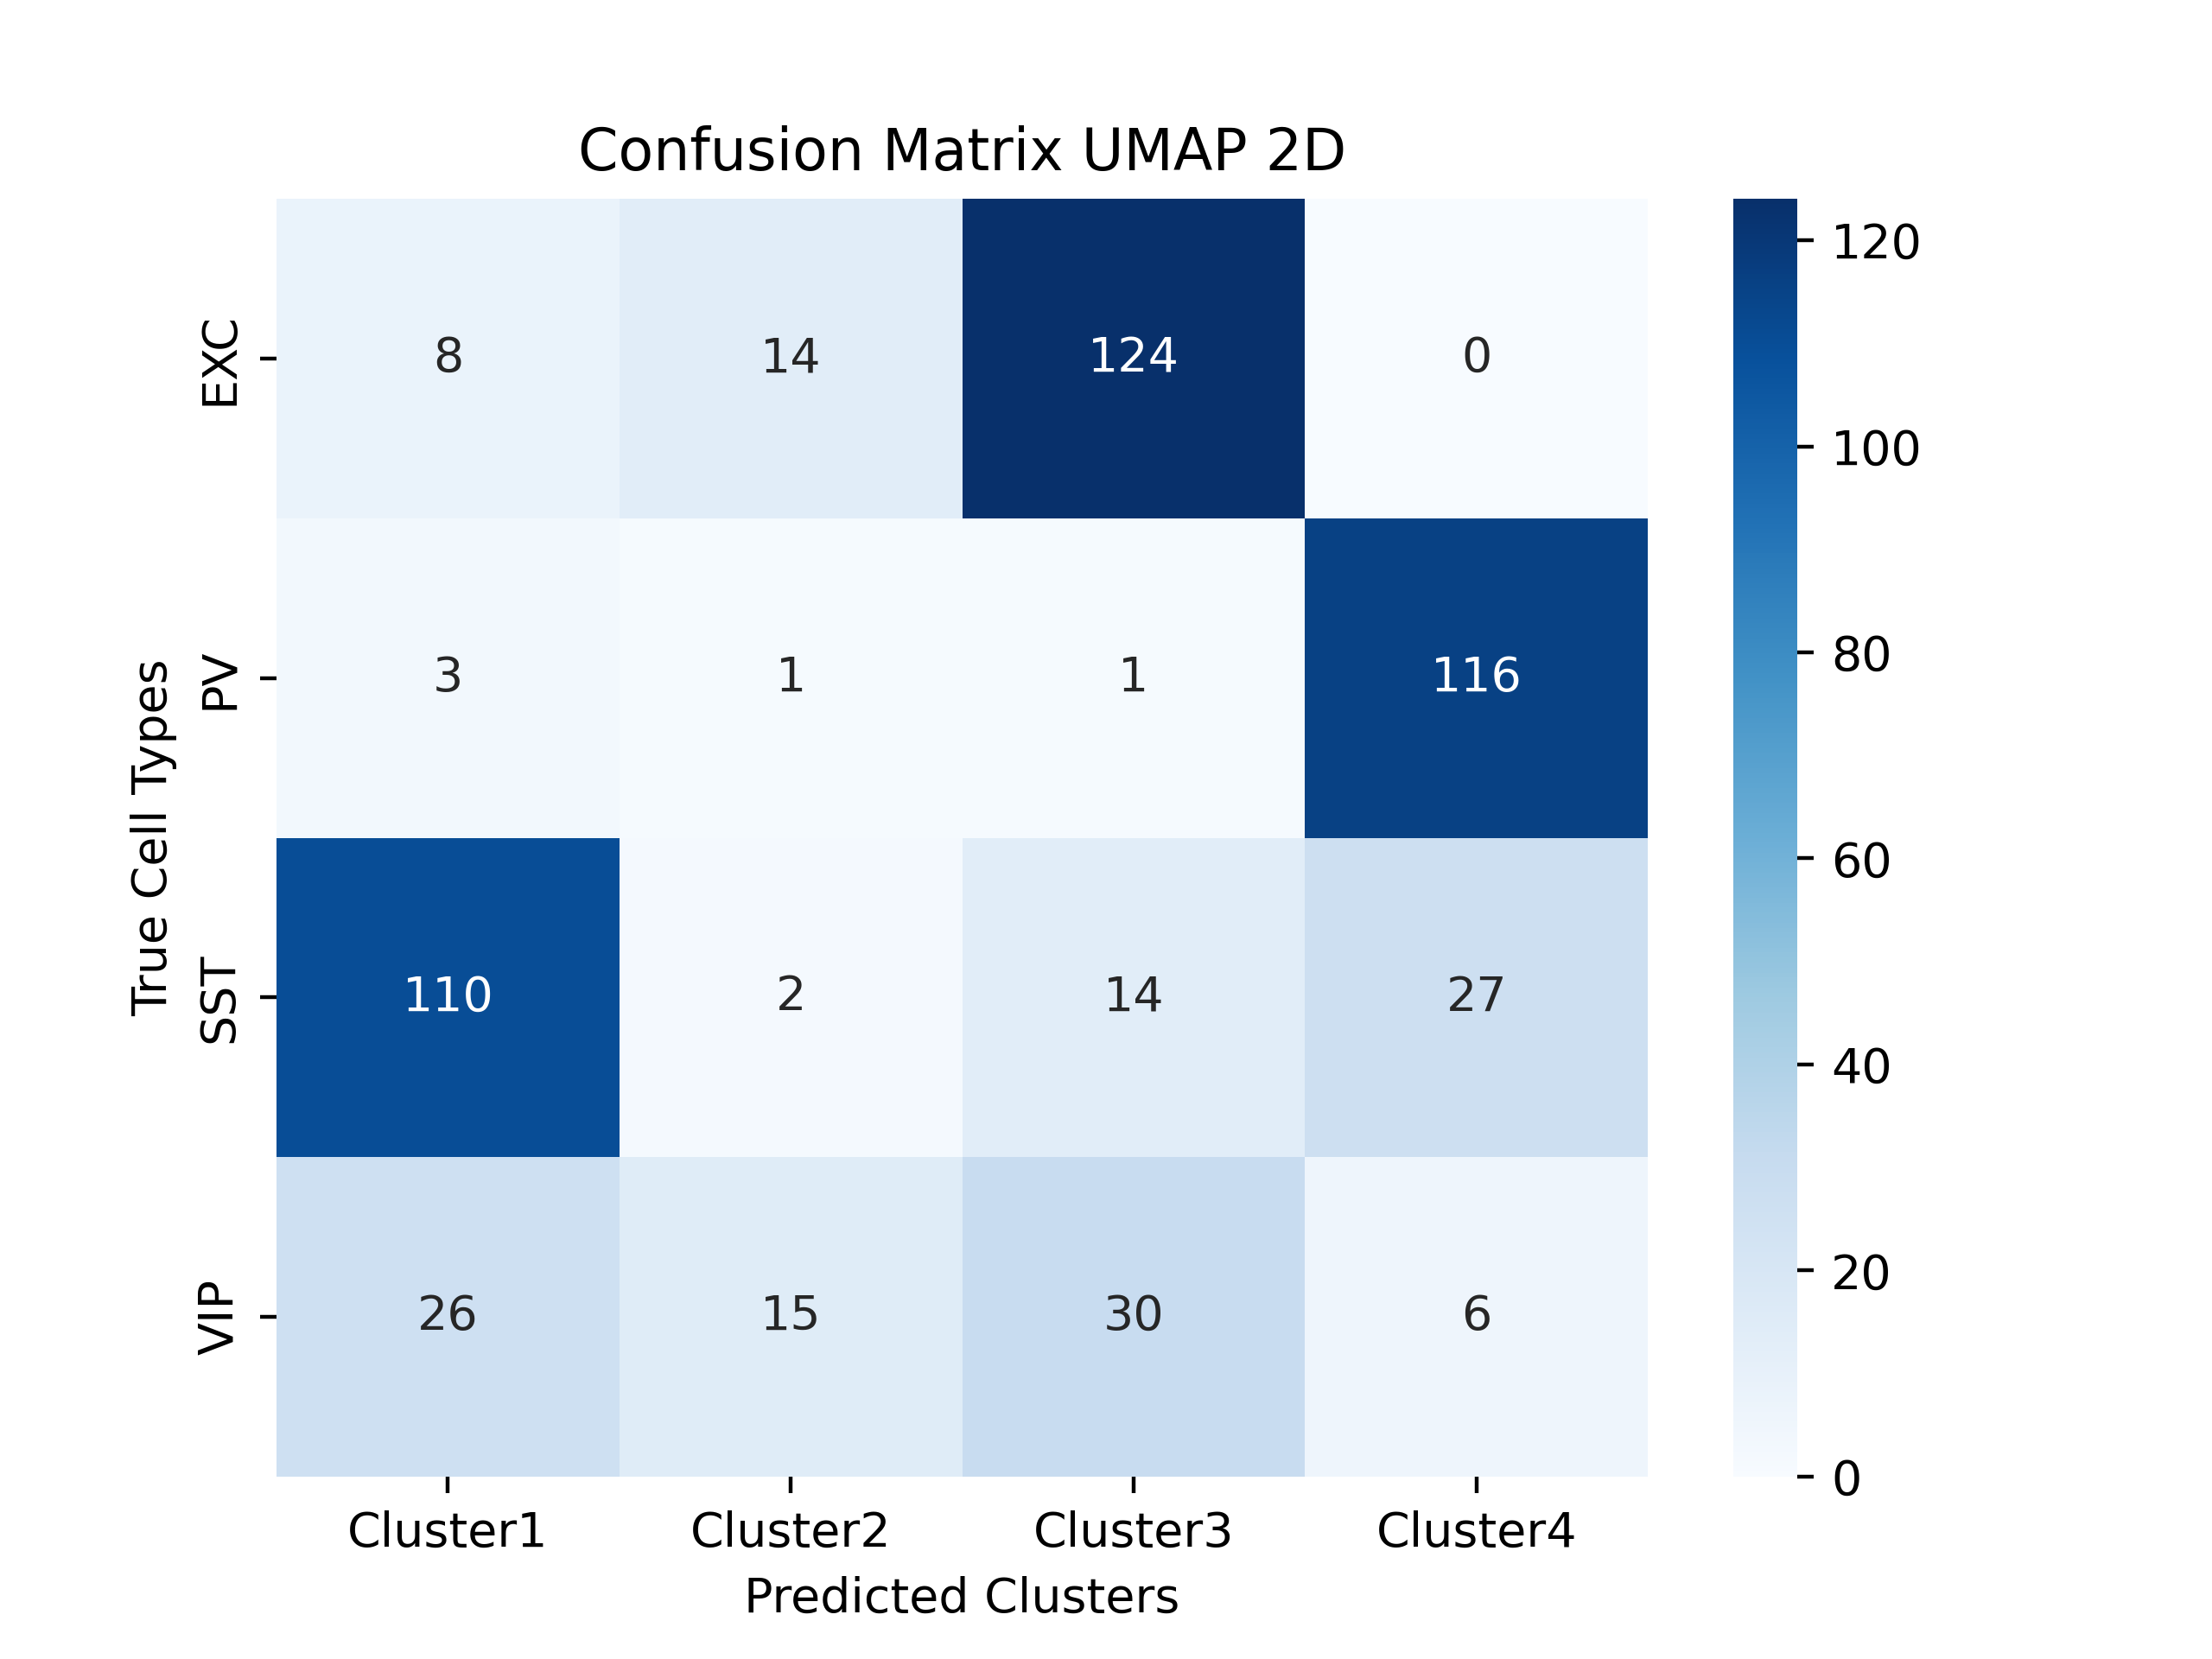
\includegraphics[width=0.45\columnwidth]{figures/Confusion Matrix UMAP 2D.png}
  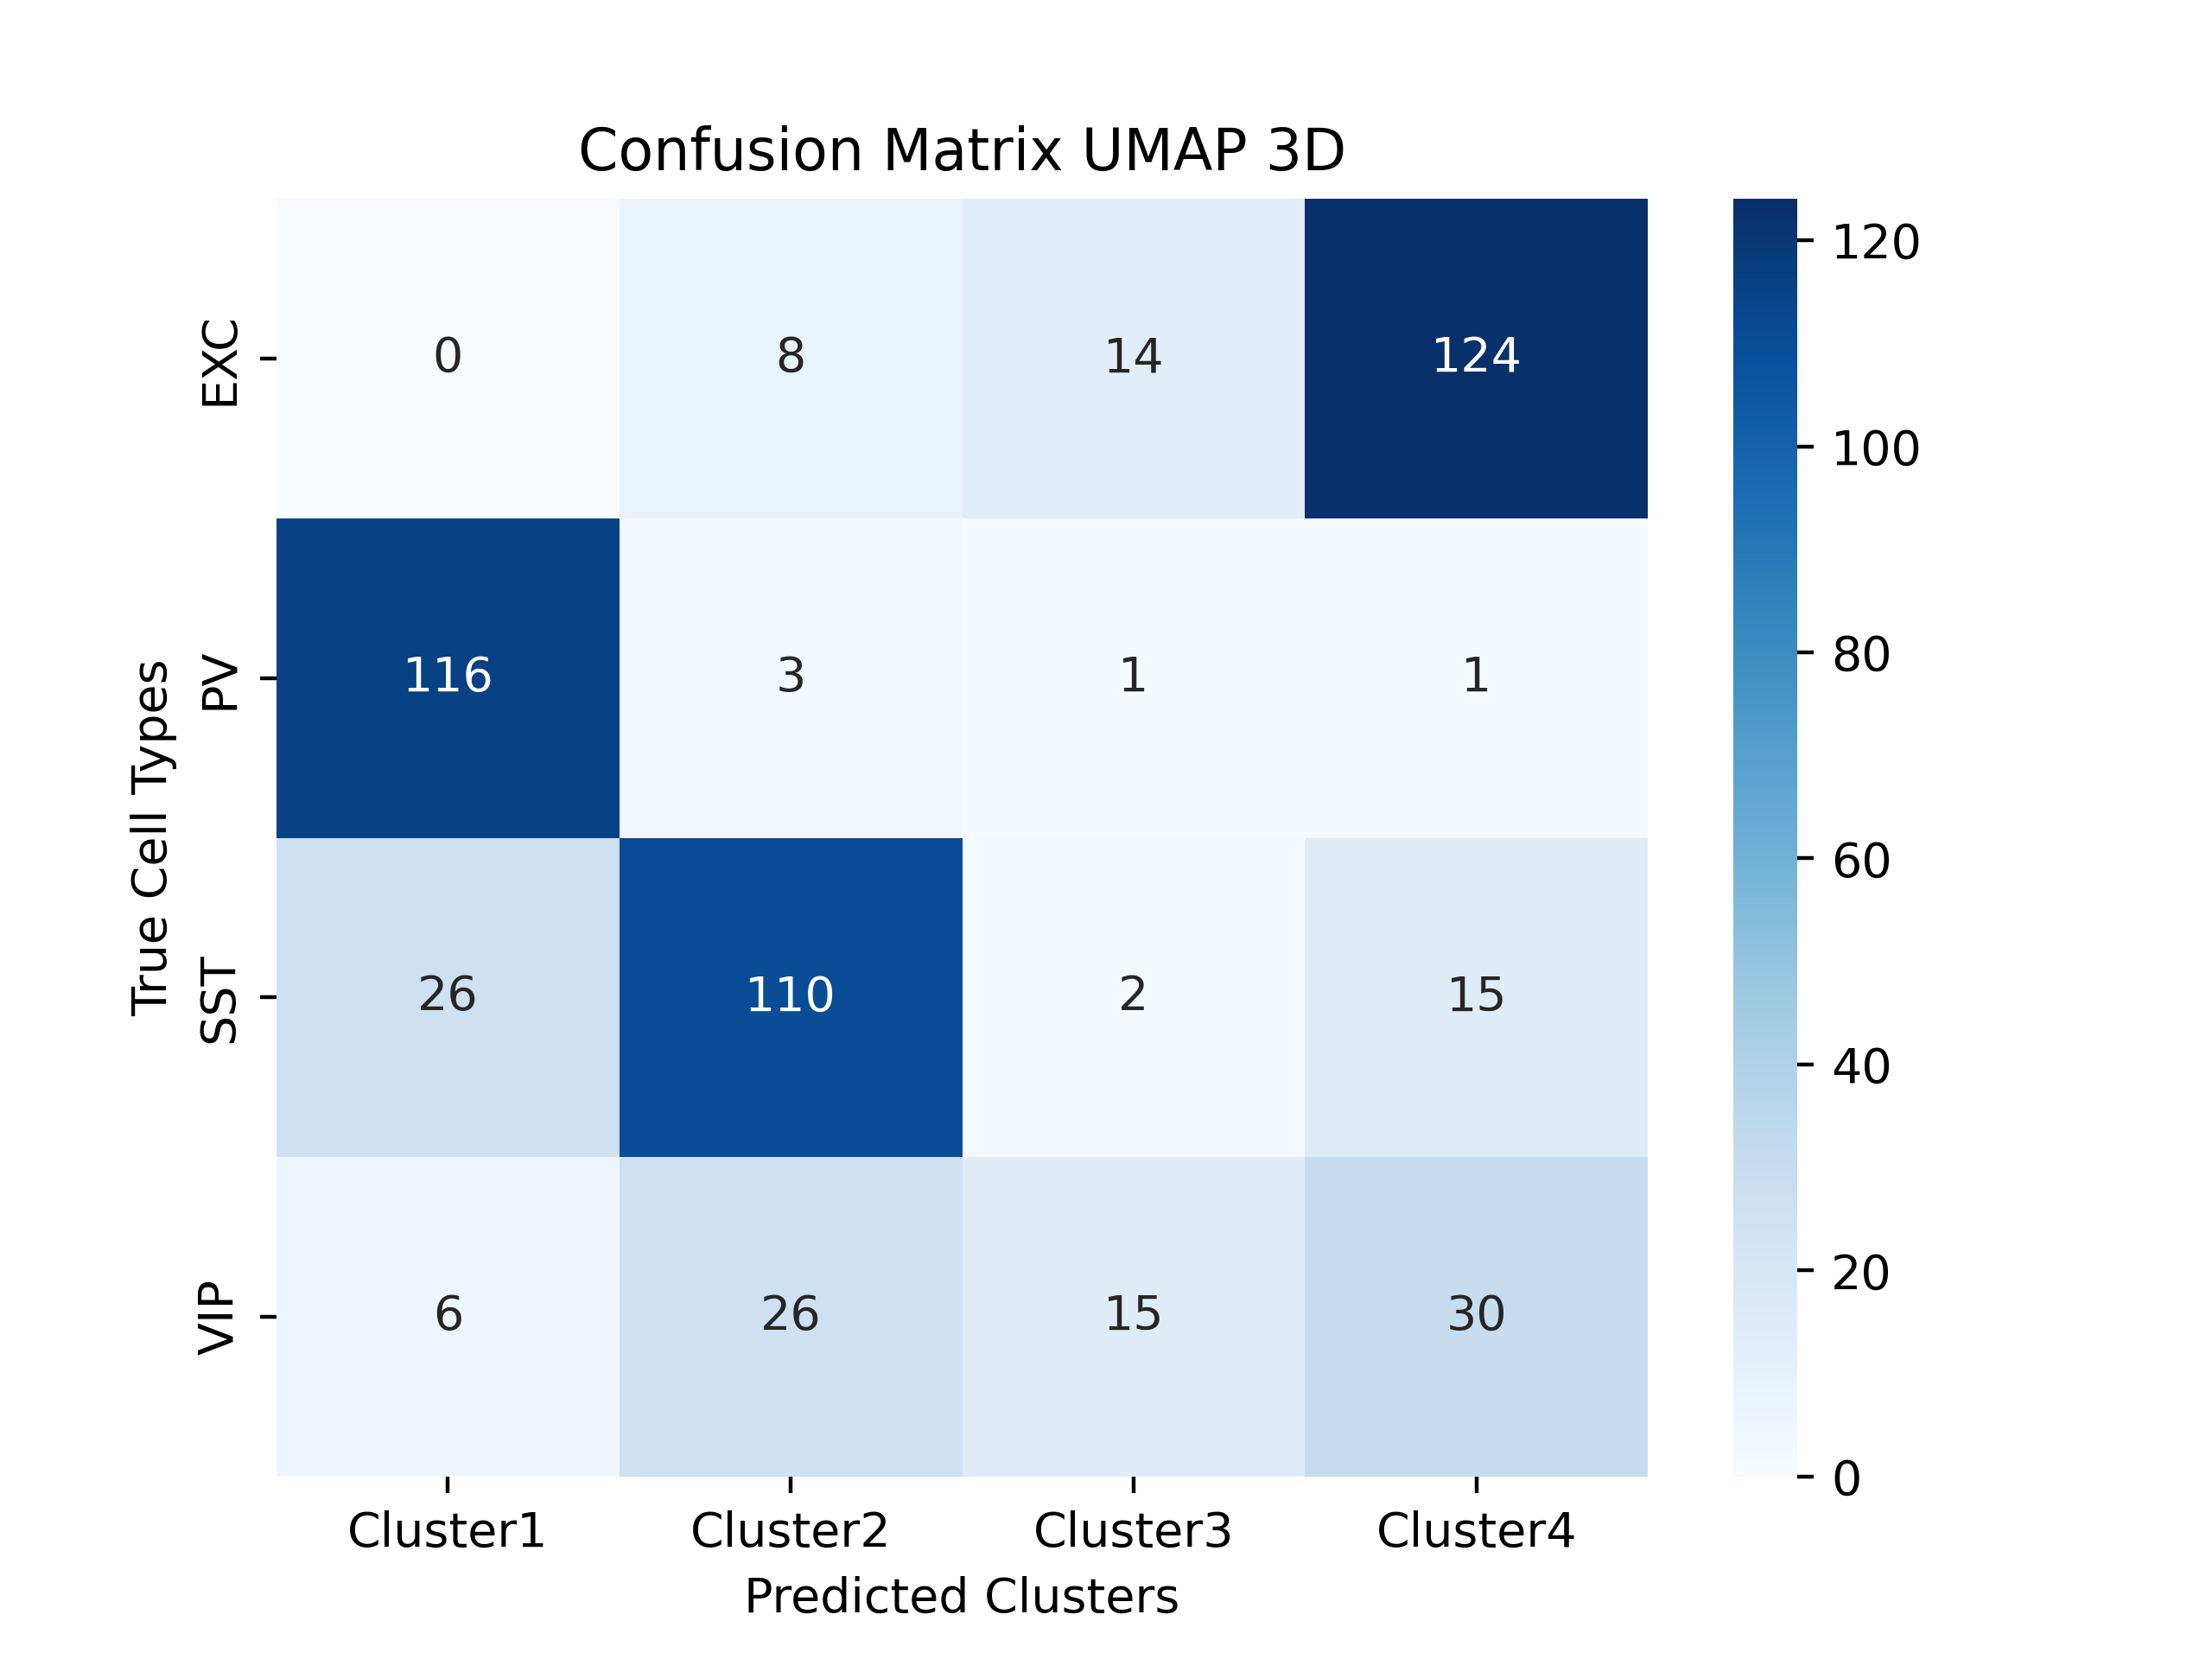
\includegraphics[width=0.45\columnwidth]{figures/Confusion Matrix UMAP 3D.png}
  \caption{K-Means Clustering Confusion Matrices. Top row is PCA. Middle row is t-SNE. Bottom row is UMAP. Left column in 2D. Right column in 3D.}%
  \label{fig:unsupervised_confusion_matrices}
\end{figure}

K-Means clustering was a majority of times able to attribute a cluster to the region with the highest density of EXC, SST and PV cells (Fig. \ref{fig:pca}, \ref{fig:t-SNE}, \ref{fig:umap}). Due to the presence of the separated mixed grouping in the bottom left corner of each different dimensional space, it is always predicted the final cluster to be there.
When looking at the confusion matrix from Fig. \ref{fig:unsupervised_confusion_matrices} one can observe the same phenomenon as described above. A cluster is always attributed to PV cells (cluster 2 and 1, for PCA, 1 and 1 for t-SNE, 4 and 1 for UMAP, respectively for 2D and 3D data). Although less pronounced, the same can be said for EXC and SST cells (except for PCA data where EXC cells are more sparse). One cluster captures the small mixed grouping consisting of roughly 14 EXC, 1 PV, 1 SST and 15 VIP cells. VIP cells are found in similar ratios within each cluster.

%-----------------------------------------------------

\section{Discussion}

\subsection{Performance}
It is important to note that for a 4-class classification like this one, a ``chance level" score is $F1_{chance}=0.25$.
In that regard, the four best models achieve above $0.87$ performance and the ensemble method is able to reach a score above $0.9$. This is quite impressive considering the relatively low sample size (n=497) and the moderate class imbalance present in our data. This means that there are definitely characteristics that can help to differentiate and discriminate between the different cell classes. Due to this high performance, we can also be more confident in our feature importance analysis.

\subsection{Cell Class Specificity}
In Fig. \ref{fig:supervised_confusion_matrices} we can see that VIP cells cannot be classified as well as the others, for every model. 
On the other hand PV cell classes are well 
Backed up by the unsupervised

The lower dimensional spatial similarity found between EXC and SST cells highlights the biological similarity between the two.

The small mixed grouping of points found bottom left of dimensionally reduced spaces (Fig. \ref{fig:pca}, \ref{fig:t-SNE}, \ref{fig:umap}), is probably due to the biologically nonsensical preprocessing step of replacing nonexistent AP durations and thresholds by a value of zero. This could mean that the 14 EXC, 1 PV, 1 SST and 15 VIP cells present in that grouping would have had no AP in their sweep.


%-----------------------------------------------------

\section{Conclusion}


%-----------------------------------------------------
\newpage
\section{Annex}

% TODO: Add this two column figure
% \begin{figure*}
%   \centering
%   \includegraphics[width=\textwidth]{figures/correlation_heatmap.png}
%   \caption{Correlation of each predictor with one another within the training data}
%   \label{fig:correlation}
% \end{figure*}

\begin{figure}[h!]%
  \centering
  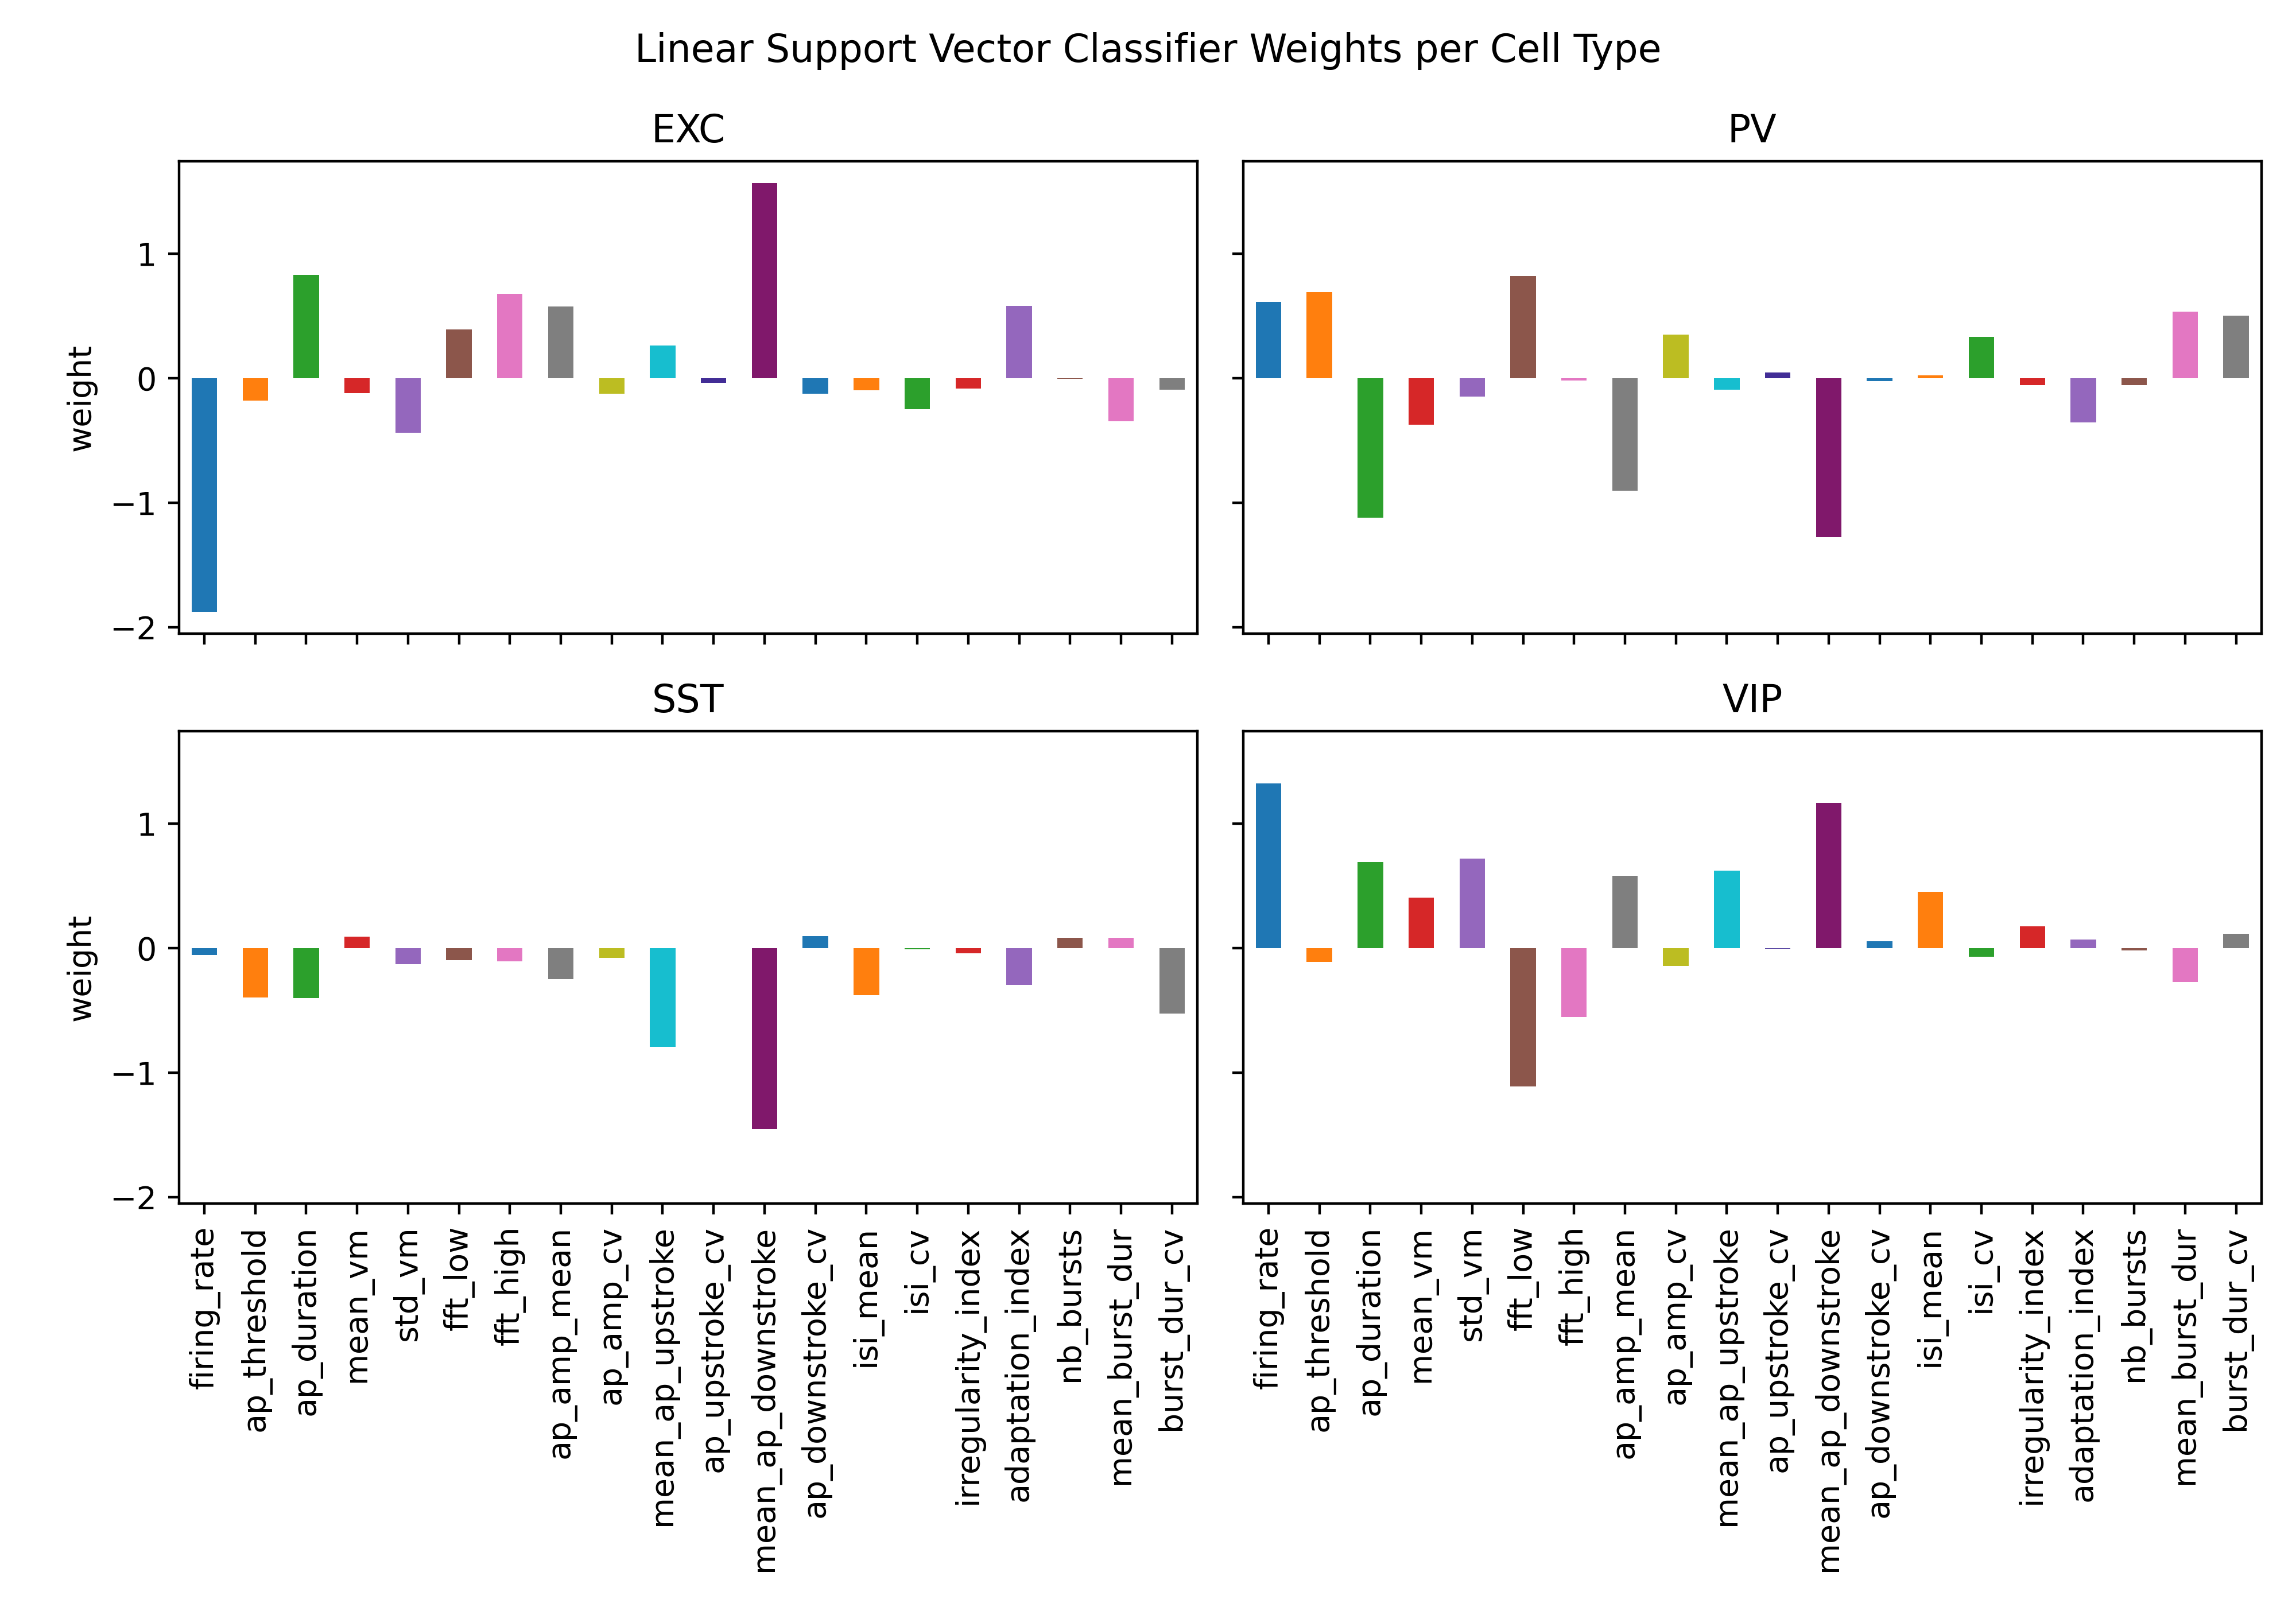
\includegraphics[width=0.9\columnwidth]{figures/weights_linearsvc.png}
  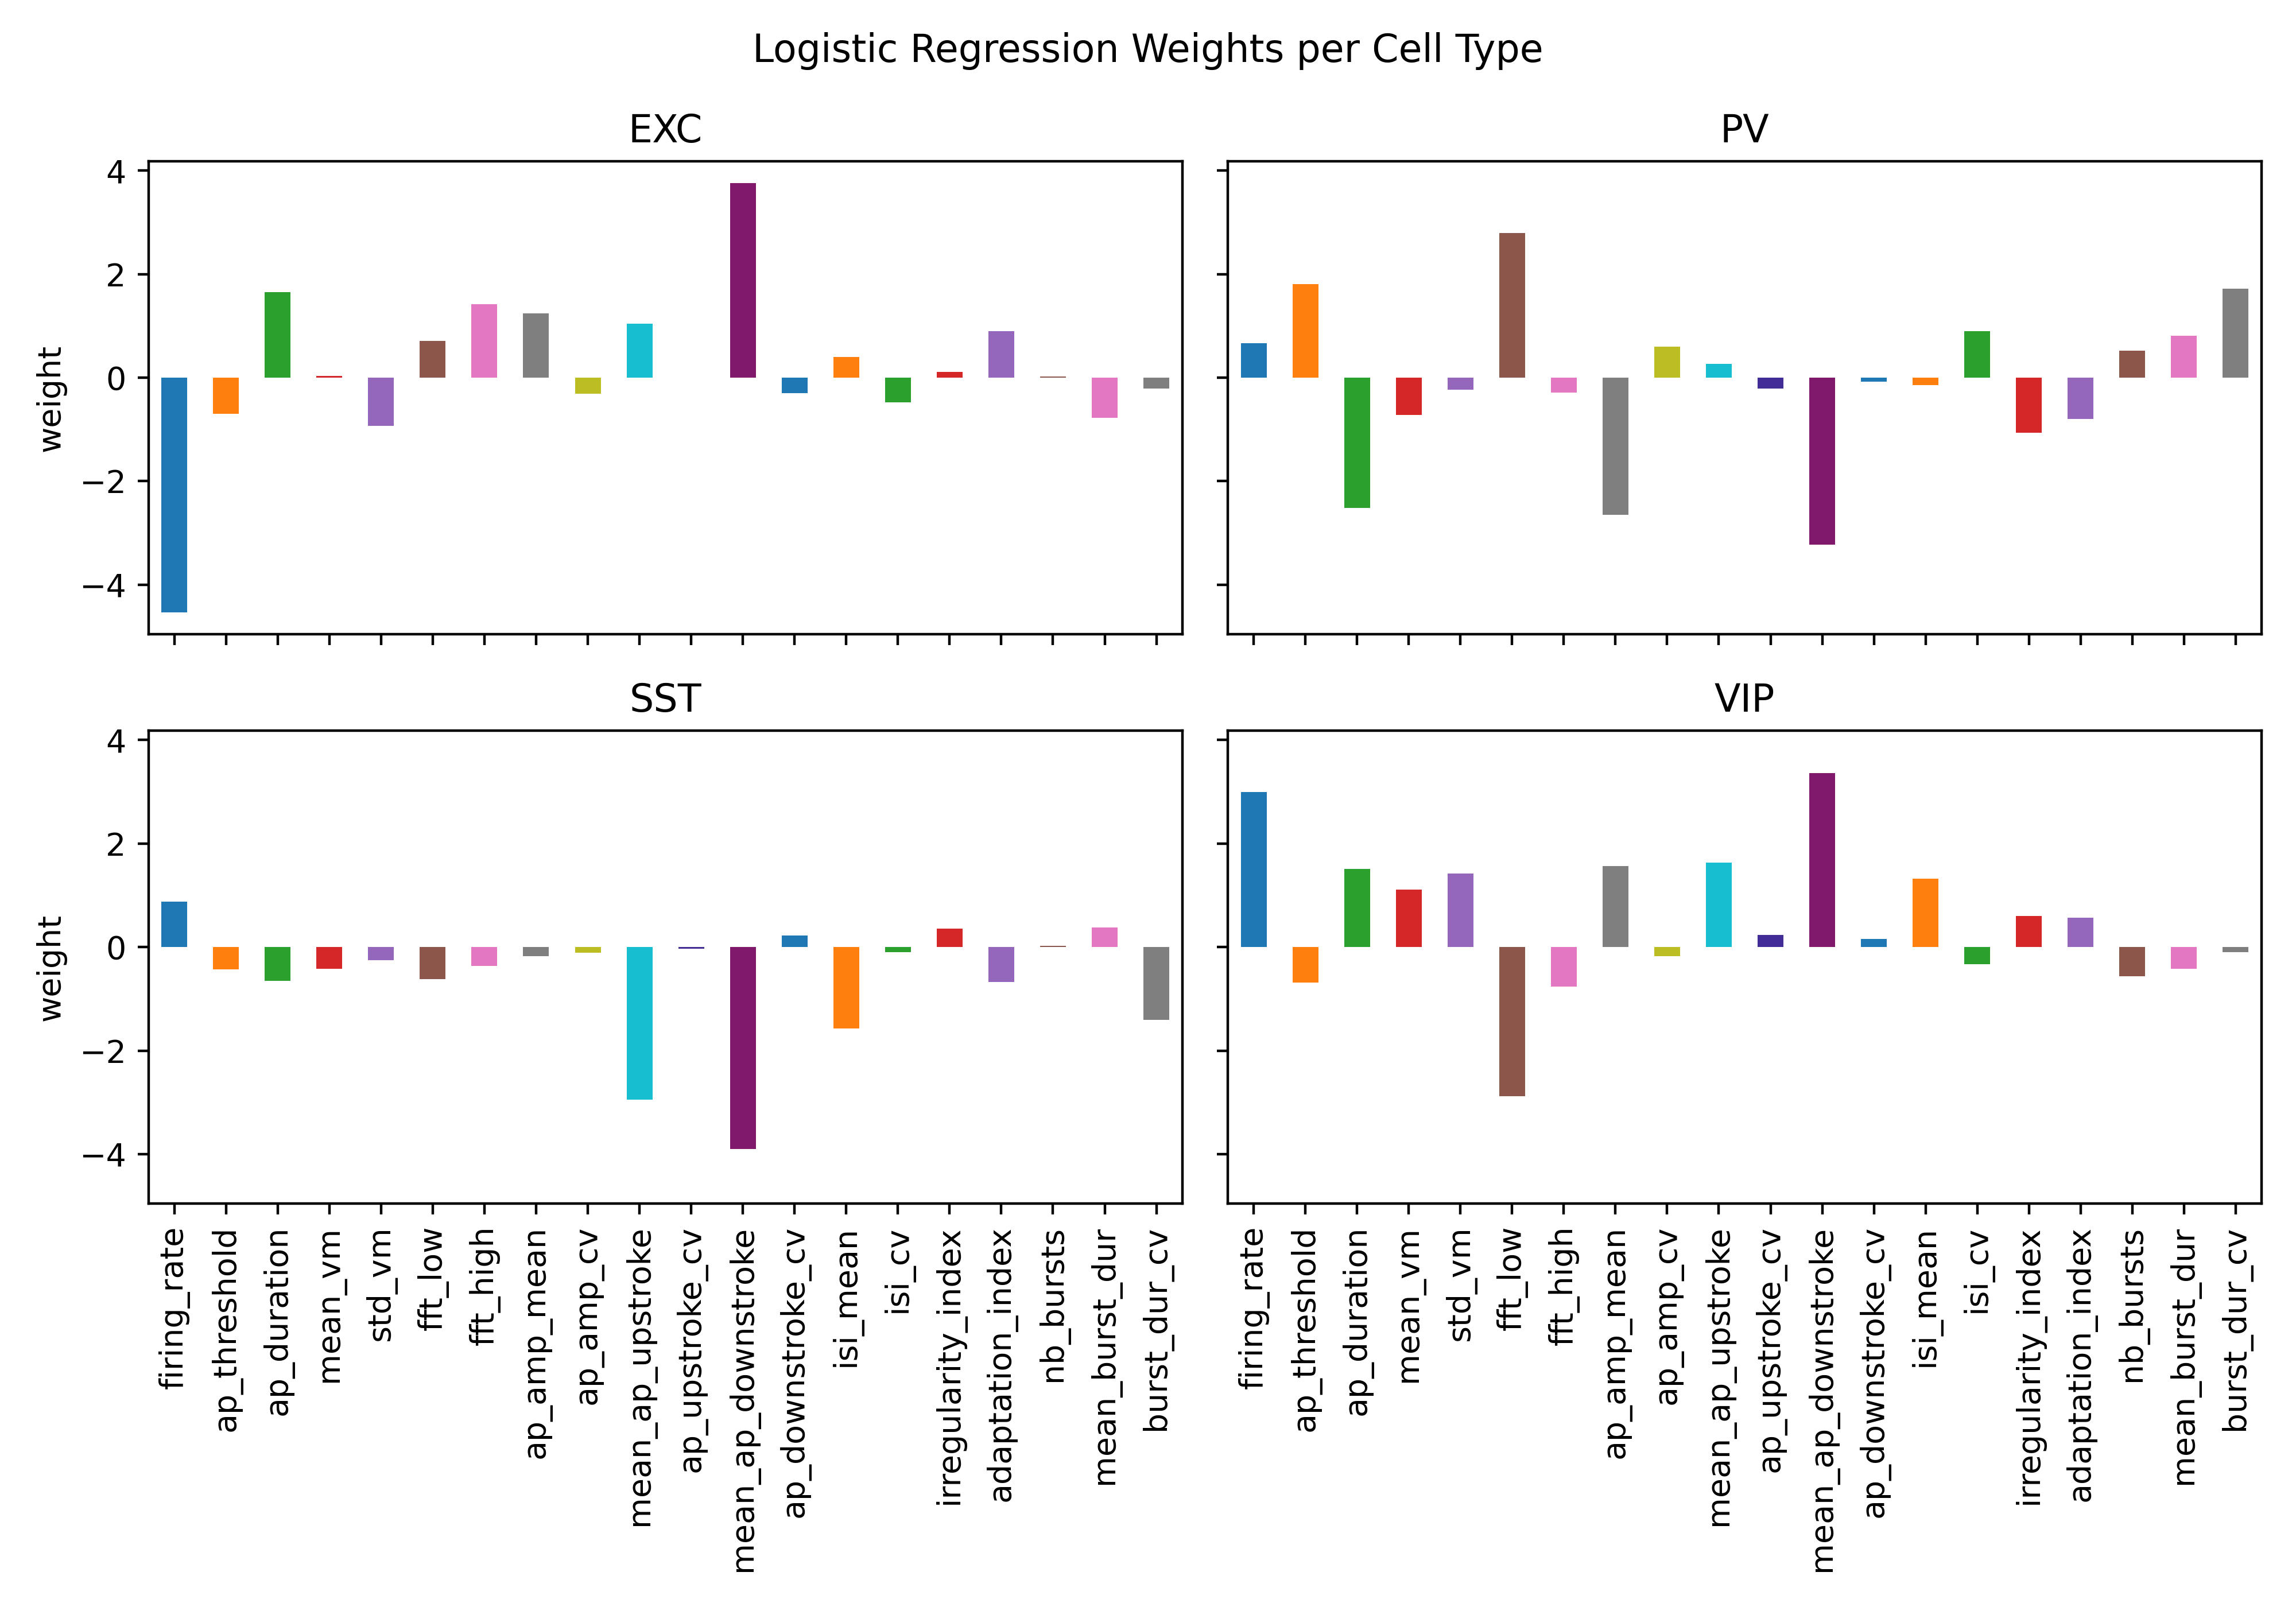
\includegraphics[width=0.9\columnwidth]{figures/weights_logistic_regression.png}
  \caption{Linear model weights across cell classes. Top four plots, are the weights of the Linear SVC (2nd best) and bottom four plots are the weights of the Logistic Regression (4th best).}%
  \label{fig:weights}
\end{figure}


\begin{table}[h!]
  \centering
  \begin{tabular}{|c|c|}
      \hline
      \textbf{Model} & \textbf{Hyperparameters} \\
      \hline
      Gradient Boosting & Learning Rate: 1.0, Max Depth: 2, N Estimators: 176 \\
      \hline
      Linear SVC & C: 0.8428, Multi-class: Crammer-Singer \\
      \hline
      Random Forest & Max Depth: 9, N Estimators: 174, Min Samples Leaf: 1 \\
      \hline
      Logistic Regression & C: 5.241 \\
      \hline
  \end{tabular}
  \caption{Hyperparameters of Different Models. Any parameter not mentioned is equal to the default parameter in Sci-kit Learn.}
  \label{tab:hyperparameters}
\end{table}


\end{document}